\section{Third - DNS}\label{third---dns}

\href{Third\%20-\%20DNS\%20263f56fc503e80ddb361c216e75fd3bf/Slackware\%20net\%20commands\%20264f56fc503e8085bd88d9584832e069.md}{Slackware
net commands}

\section{SLACKWARE - PRYMARY DNS ✅}\label{slackware---prymary-dns}

Perfect! Let's complete Point 1 step by step. Since you have 2 students,
we'll configure 2 domains.

\subsection{Step 1: Plan Your
Configuration}\label{step-1-plan-your-configuration}

First, let's define your domains and servers:

\textbf{Replace these with your actual names:}

\begin{itemize}
\tightlist
\item
  Domain 1: \texttt{cristian.com.it}
\item
  Domain 2:\texttt{andersson.org.uk}
\end{itemize}

\textbf{Server Distribution:}

\begin{itemize}
\tightlist
\item
  \textbf{Domain 1 (cristian.com.it)}: Primary on Solaris, Secondary on
  Slackware + Windows
\item
  \textbf{Domain 2 (andersson.org.uk)}: Primary on Slackware, Secondary
  on Solaris + Windows
\end{itemize}

\subsection{Step 2: Start with Slackware (Primary DNS for Domain
2)}\label{step-2-start-with-slackware-primary-dns-for-domain-2}

\subsubsection{2.0. Check if BIND is already
installed}\label{check-if-bind-is-already-installed}

\begin{Shaded}
\begin{Highlighting}[]

\ExtensionTok{*which}\NormalTok{ named}\PreprocessorTok{*}
\ExtensionTok{*ls}\NormalTok{ /usr/sbin/named}\PreprocessorTok{*}
\end{Highlighting}
\end{Shaded}

If you see \texttt{/usr/sbin/named}, BIND is already installed! Skip to
step 4.

\begin{figure}
\centering
\pandocbounded{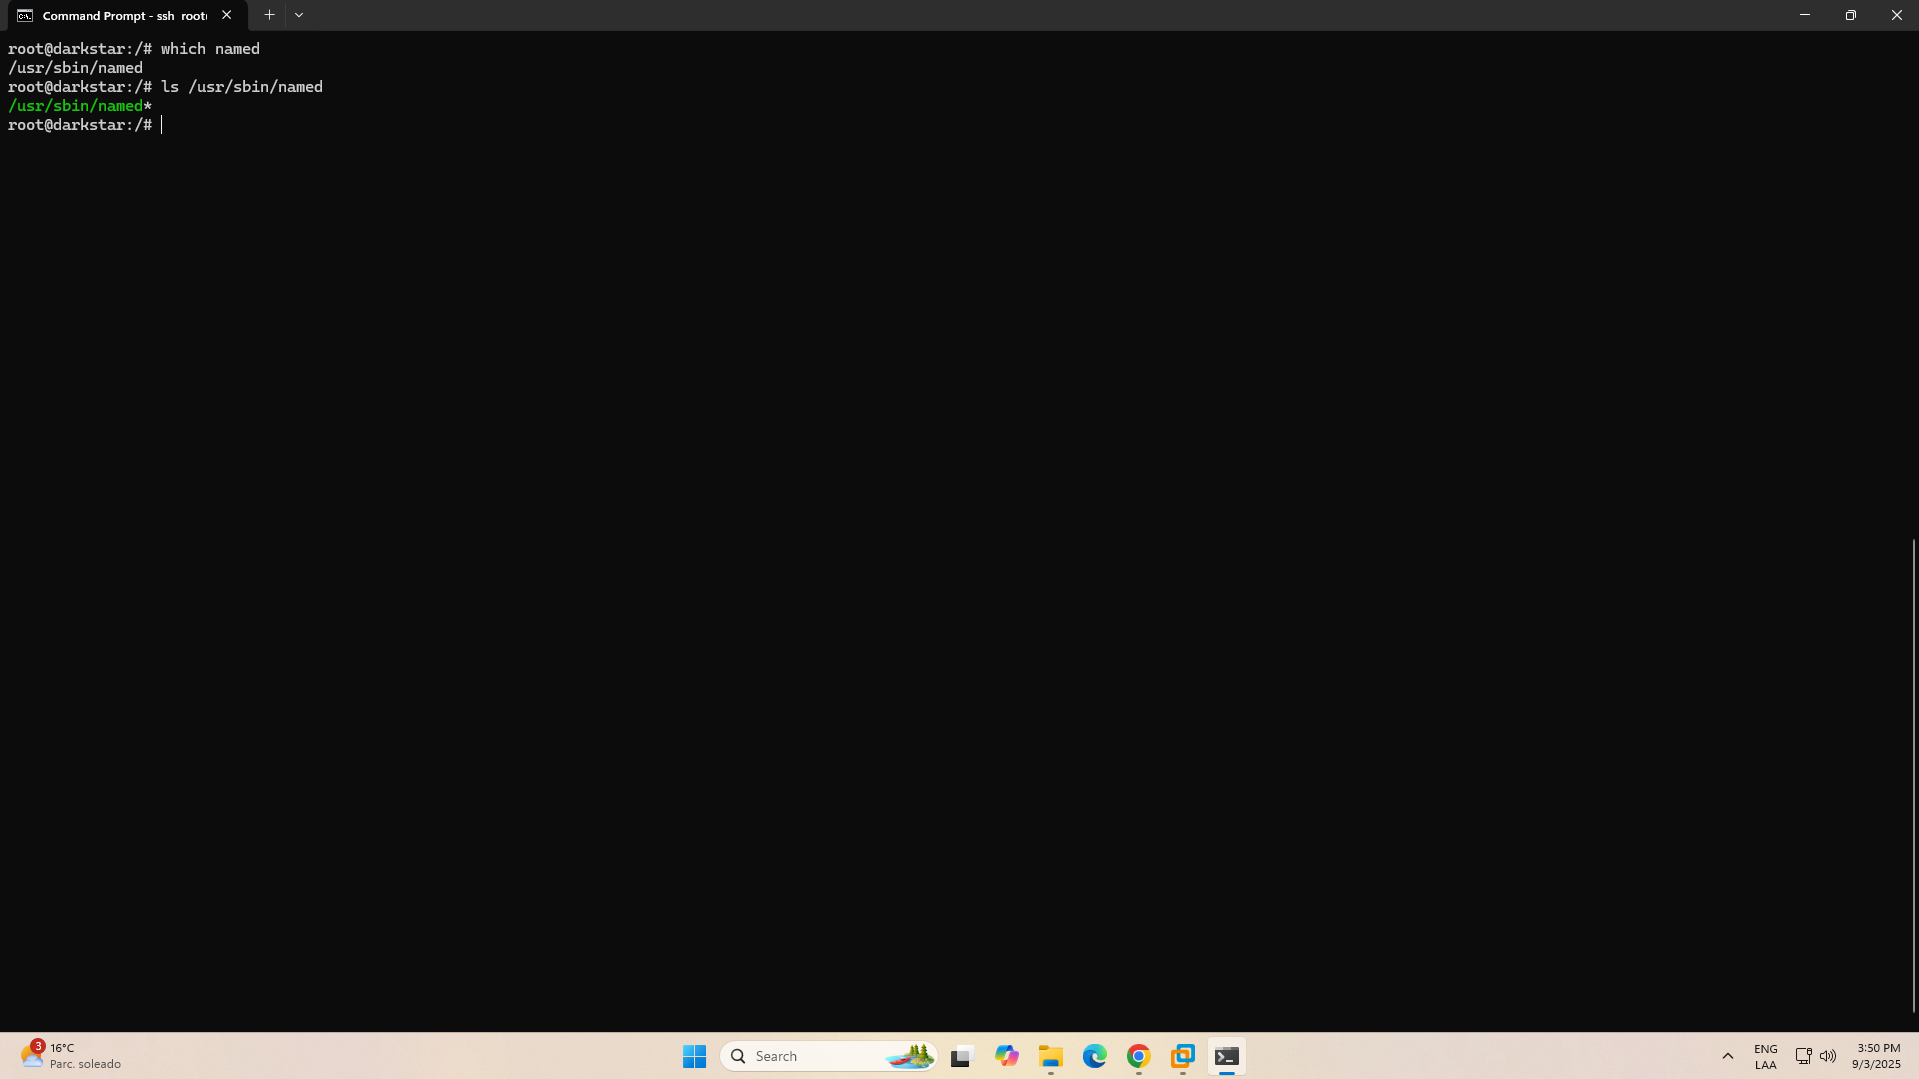
\includegraphics[keepaspectratio,alt={image.png}]{Third - DNS 263f56fc503e80ddb361c216e75fd3bf/image.png}}
\caption{image.png}
\end{figure}

\subsubsection{\texorpdfstring{\st{2.1 Install BIND (if
needed)}}{2.1 Install BIND (if needed)}}\label{install-bind-if-needed}

\begin{Shaded}
\begin{Highlighting}[]
\CommentTok{\# Mount the CD/ISO and install BIND}
\FunctionTok{mount}\NormalTok{ /dev/cdrom /mnt/cdrom}
\BuiltInTok{cd}\NormalTok{ /mnt/cdrom/slackware}\PreprocessorTok{*}
\ExtensionTok{installpkg}\NormalTok{ bind}\PreprocessorTok{*}\NormalTok{.txz}
\FunctionTok{umount}\NormalTok{ /mnt/cdrom}
\end{Highlighting}
\end{Shaded}

\subsubsection{2.2 Create the main configuration
file}\label{create-the-main-configuration-file}

\begin{Shaded}
\begin{Highlighting}[]
\FunctionTok{nano}\NormalTok{ /etc/named.conf}
\end{Highlighting}
\end{Shaded}

\textbf{This is the configuration}

\begin{Shaded}
\begin{Highlighting}[]
\ExtensionTok{options}\NormalTok{ \{}
        \ExtensionTok{directory} \StringTok{"/var/named"}\KeywordTok{;}
        \ExtensionTok{allow{-}query}\NormalTok{ \{ any}\KeywordTok{;} \ErrorTok{\}}\KeywordTok{;}
        \ExtensionTok{recursion}\NormalTok{ yes}\KeywordTok{;}
\ErrorTok{\}}\KeywordTok{;}

\ExtensionTok{//}\NormalTok{ Root zone}
\ExtensionTok{zone} \StringTok{"."}\NormalTok{ IN \{}
        \BuiltInTok{type}\NormalTok{ hint}\KeywordTok{;}
        \FunctionTok{file} \StringTok{"caching{-}example/named.root"}\KeywordTok{;}
\ErrorTok{\}}\KeywordTok{;}

\ExtensionTok{//}\NormalTok{ PRIMARY zone for andersson.org.uk}
\ExtensionTok{zone} \StringTok{"andersson.org.uk"}\NormalTok{ IN \{}
        \BuiltInTok{type}\NormalTok{ master}\KeywordTok{;}
        \FunctionTok{file} \StringTok{"andersson.org.uk.zone"}\KeywordTok{;}
\ErrorTok{\}}\KeywordTok{;}

\ExtensionTok{//}\NormalTok{ Localhost zones}
\ExtensionTok{zone} \StringTok{"localhost"}\NormalTok{ IN \{}
        \BuiltInTok{type}\NormalTok{ master}\KeywordTok{;}
        \FunctionTok{file} \StringTok{"caching{-}example/localhost.zone"}\KeywordTok{;}
        \ExtensionTok{allow{-}update}\NormalTok{ \{ none}\KeywordTok{;} \ErrorTok{\}}\KeywordTok{;}
\ErrorTok{\}}\KeywordTok{;}

\ExtensionTok{zone} \StringTok{"0.0.127.in{-}addr.arpa"}\NormalTok{ IN \{}
        \BuiltInTok{type}\NormalTok{ master}\KeywordTok{;}
        \FunctionTok{file} \StringTok{"caching{-}example/named.local"}\KeywordTok{;}
        \ExtensionTok{allow{-}update}\NormalTok{ \{ none}\KeywordTok{;} \ErrorTok{\}}\KeywordTok{;}
        
       
\ErrorTok{\}}\KeywordTok{;}
\end{Highlighting}
\end{Shaded}

\begin{figure}
\centering
\pandocbounded{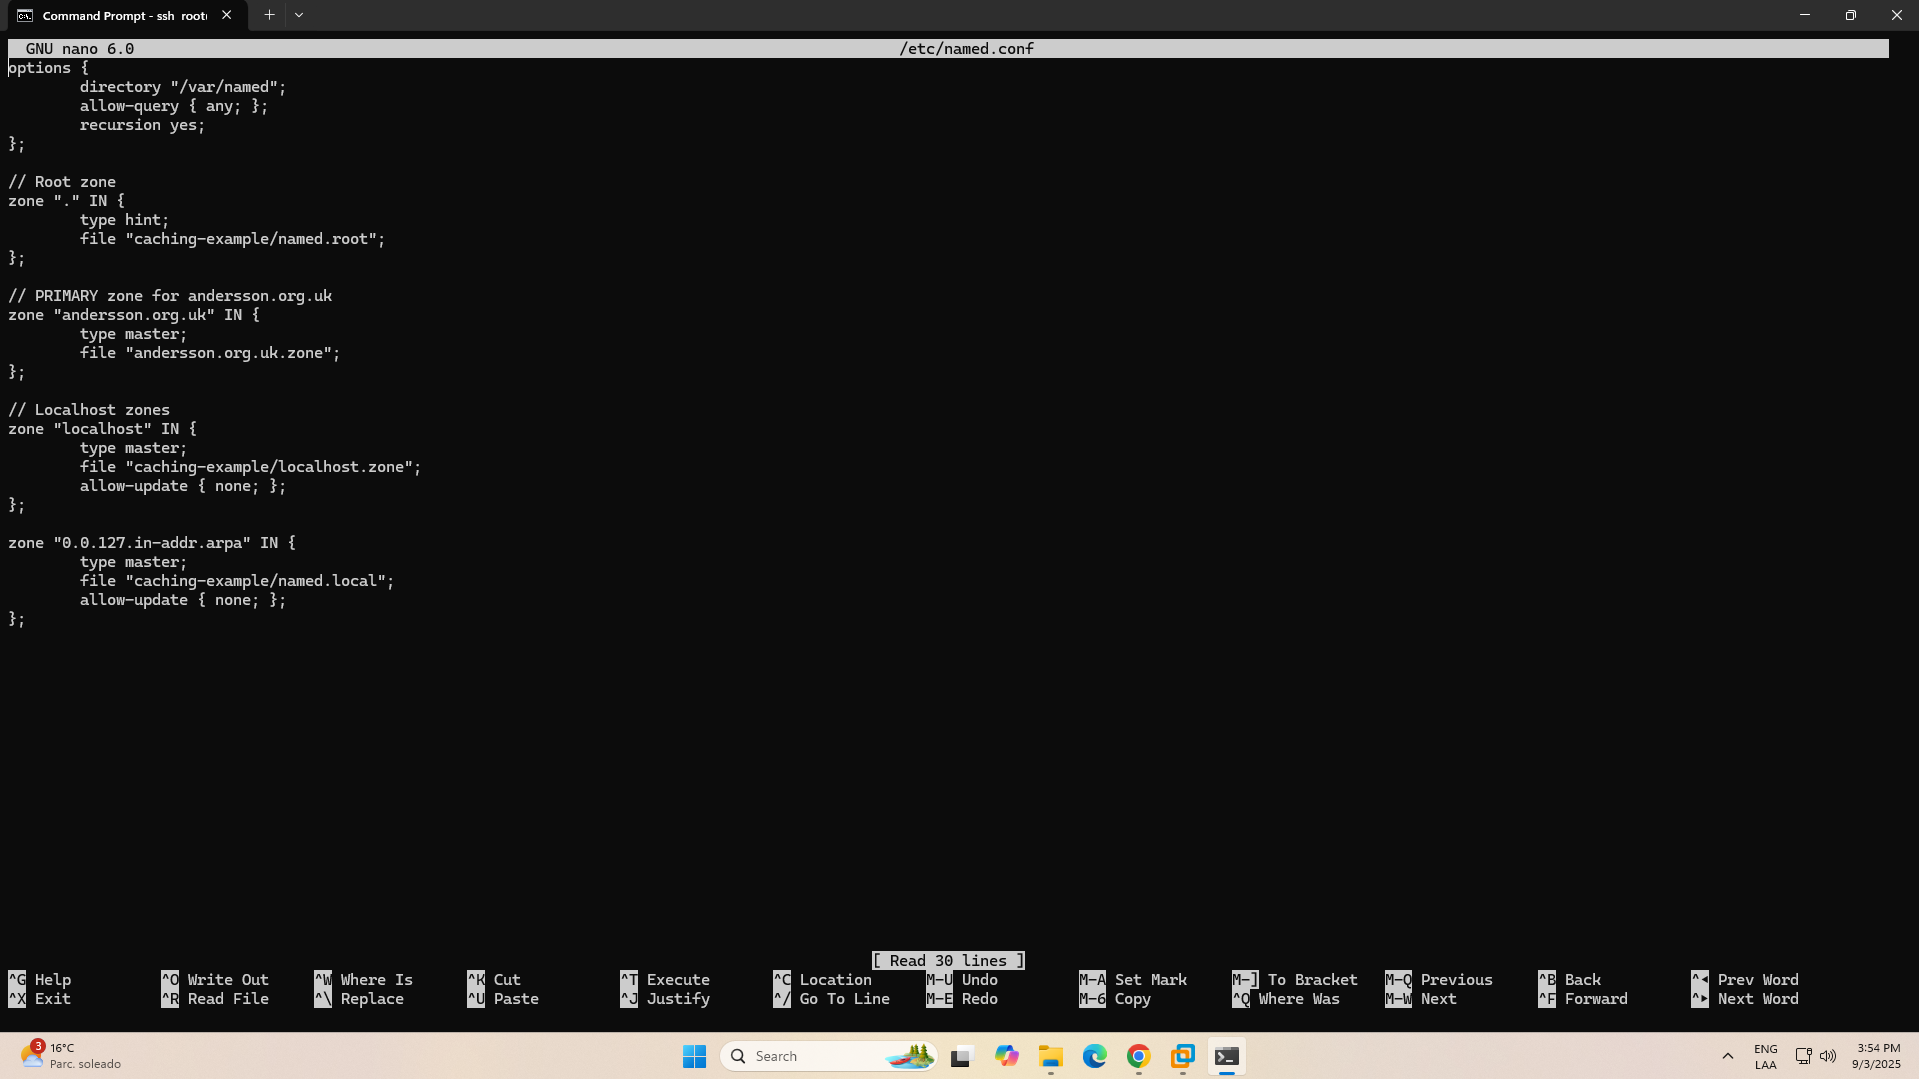
\includegraphics[keepaspectratio,alt={image.png}]{Third - DNS 263f56fc503e80ddb361c216e75fd3bf/image 1.png}}
\caption{image.png}
\end{figure}

\subsubsection{2.4 Create the SOA file}\label{create-the-soa-file}

\begin{Shaded}
\begin{Highlighting}[]
\FunctionTok{nano}\NormalTok{ /var/named/andersson.soa}
\end{Highlighting}
\end{Shaded}

\textbf{Copy this content (}

\begin{Shaded}
\begin{Highlighting}[]
\KeywordTok{;}
\KeywordTok{;} \ExtensionTok{SOA}\NormalTok{ record for andersson.org.uk}
\KeywordTok{;}
\ExtensionTok{@}\NormalTok{ IN SOA dns.andersson.org.uk. admin.andersson.org.uk. }\ErrorTok{(}
    \ExtensionTok{2024120301}  \KeywordTok{;} \ExtensionTok{Serial} \ErrorTok{(}\ExtensionTok{YYYYMMDDXX}\KeywordTok{)}
    \ExtensionTok{3600}        \KeywordTok{;} \ExtensionTok{Refresh} \ErrorTok{(}\ExtensionTok{1}\NormalTok{ hour}\KeywordTok{)}
    \ExtensionTok{1800}        \KeywordTok{;} \ExtensionTok{Retry} \ErrorTok{(}\ExtensionTok{30}\NormalTok{ minutes}\KeywordTok{)}
    \ExtensionTok{604800}      \KeywordTok{;} \ExtensionTok{Expire} \ErrorTok{(}\ExtensionTok{1}\NormalTok{ week}\KeywordTok{)}
    \ExtensionTok{86400}       \KeywordTok{;} \ExtensionTok{Minimum}\NormalTok{ TTL }\ErrorTok{(}\ExtensionTok{1}\NormalTok{ day}\KeywordTok{)}
\KeywordTok{)}
\end{Highlighting}
\end{Shaded}

\begin{figure}
\centering
\pandocbounded{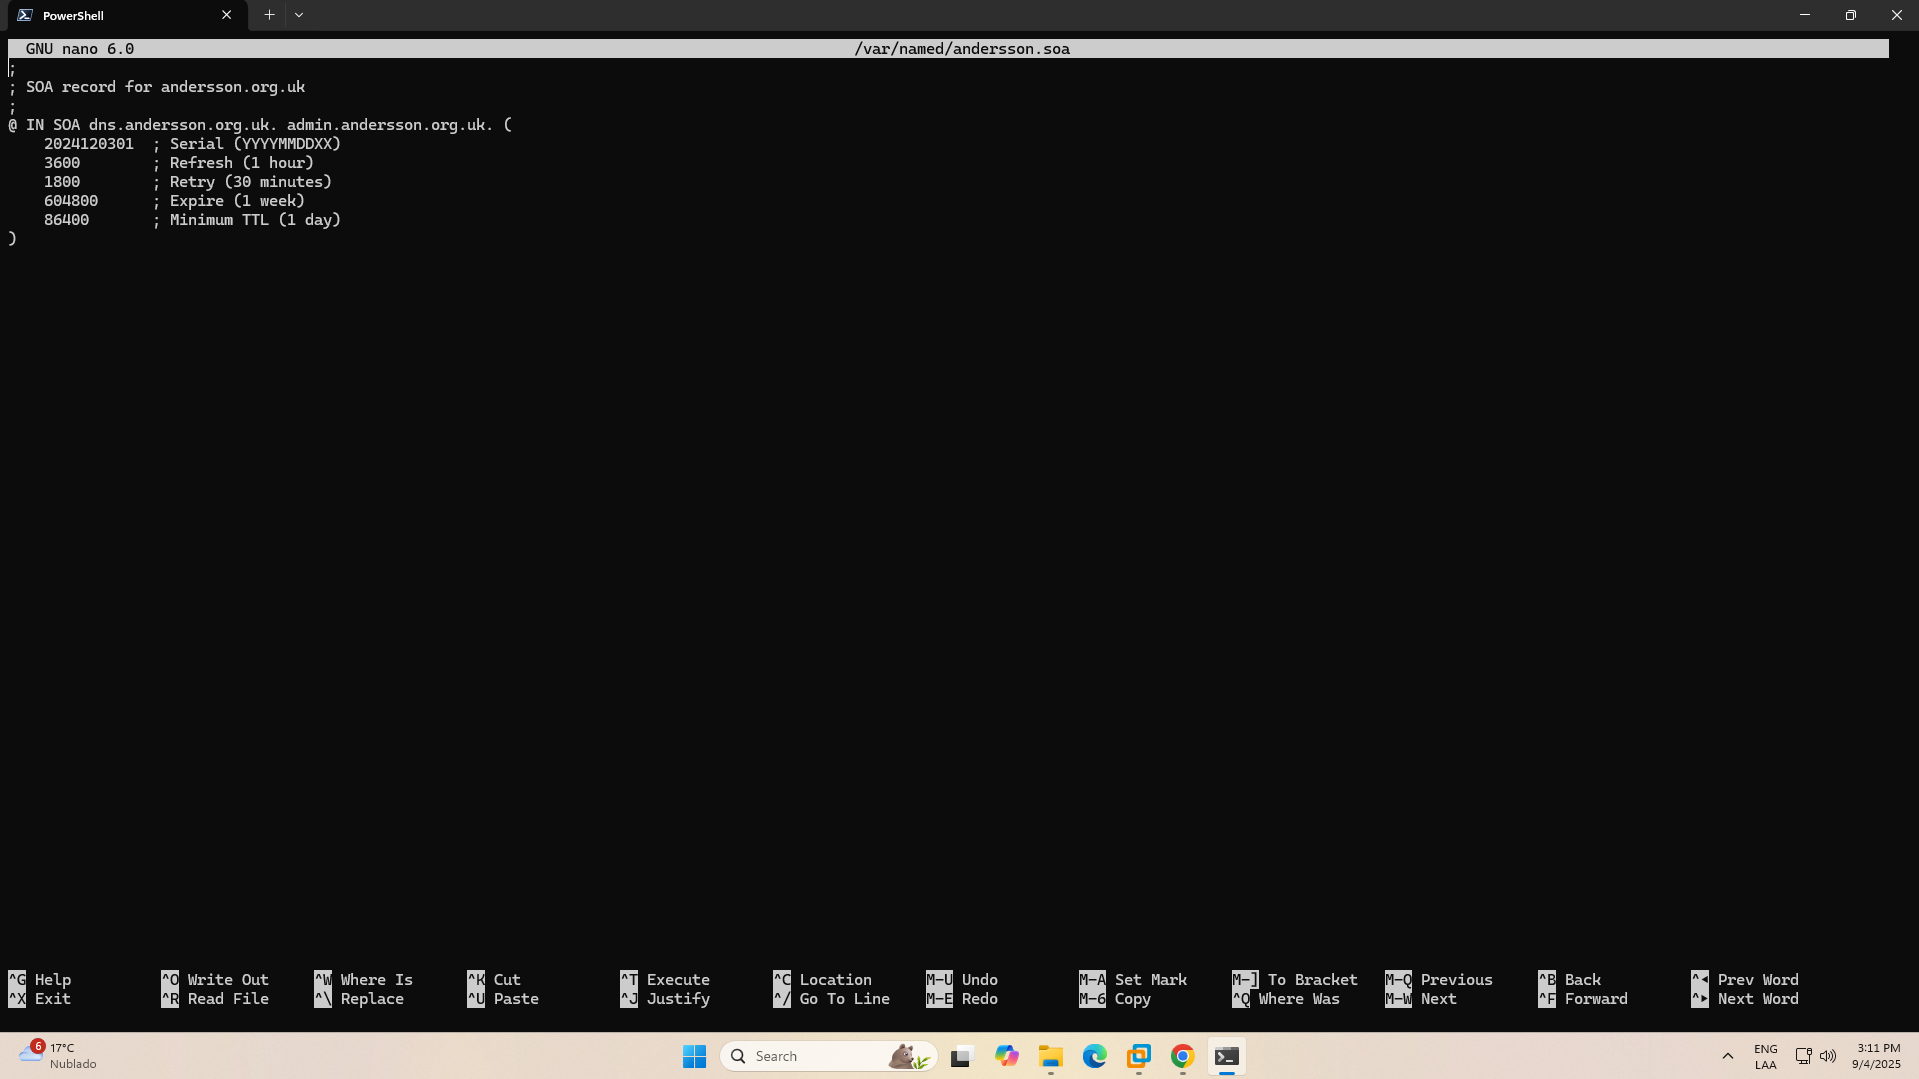
\includegraphics[keepaspectratio,alt={image.png}]{Third - DNS 263f56fc503e80ddb361c216e75fd3bf/image 2.png}}
\caption{image.png}
\end{figure}

\subsubsection{2.4 Create the domain hosts
file}\label{create-the-domain-hosts-file}

\begin{Shaded}
\begin{Highlighting}[]
\FunctionTok{nano}\NormalTok{ /var/named/andersson.org.uk.zone}
\end{Highlighting}
\end{Shaded}

\textbf{Copy this content (replace IPs with your assigned range):}

\begin{Shaded}
\begin{Highlighting}[]
\KeywordTok{;}
\KeywordTok{;} \ExtensionTok{Zone}\NormalTok{ file for andersson.org.uk}
\KeywordTok{;}
\VariableTok{$INCLUDE}\NormalTok{ andersson.soa}

\KeywordTok{;} \ExtensionTok{Name}\NormalTok{ Server}
\ExtensionTok{andersson.org.uk.}\NormalTok{ IN NS dns.andersson.org.uk.}

\KeywordTok{;} \ExtensionTok{IPv4}\NormalTok{ addresses }\ErrorTok{(}\ExtensionTok{A}\NormalTok{ records}\KeywordTok{)} \ExtensionTok{{-}}\NormalTok{ Usando tu rango real}
\ExtensionTok{dns.andersson.org.uk.}\NormalTok{     IN A 10.2.77.176}
\ExtensionTok{server1.andersson.org.uk.}\NormalTok{ IN A 10.2.77.177}
\ExtensionTok{server2.andersson.org.uk.}\NormalTok{ IN A 10.2.77.178}
\ExtensionTok{server3.andersson.org.uk.}\NormalTok{ IN A 10.2.77.179}

\KeywordTok{;} \ExtensionTok{IPv6}\NormalTok{ addresses }\ErrorTok{(}\ExtensionTok{AAAA}\NormalTok{ records}\KeywordTok{)}
\ExtensionTok{server1.andersson.org.uk.}\NormalTok{ IN AAAA 2001:db8::1}
\ExtensionTok{server2.andersson.org.uk.}\NormalTok{ IN AAAA 2001:db8::2}

\KeywordTok{;} \ExtensionTok{Aliases} \ErrorTok{(}\ExtensionTok{CNAME}\NormalTok{ records}\KeywordTok{)}
\ExtensionTok{www.andersson.org.uk.}\NormalTok{     IN CNAME server1.andersson.org.uk.}
\ExtensionTok{mail.andersson.org.uk.}\NormalTok{    IN CNAME server2.andersson.org.uk.}
\ExtensionTok{web.andersson.org.uk.}\NormalTok{     IN CNAME server1.andersson.org.uk.}
\end{Highlighting}
\end{Shaded}

\begin{figure}
\centering
\pandocbounded{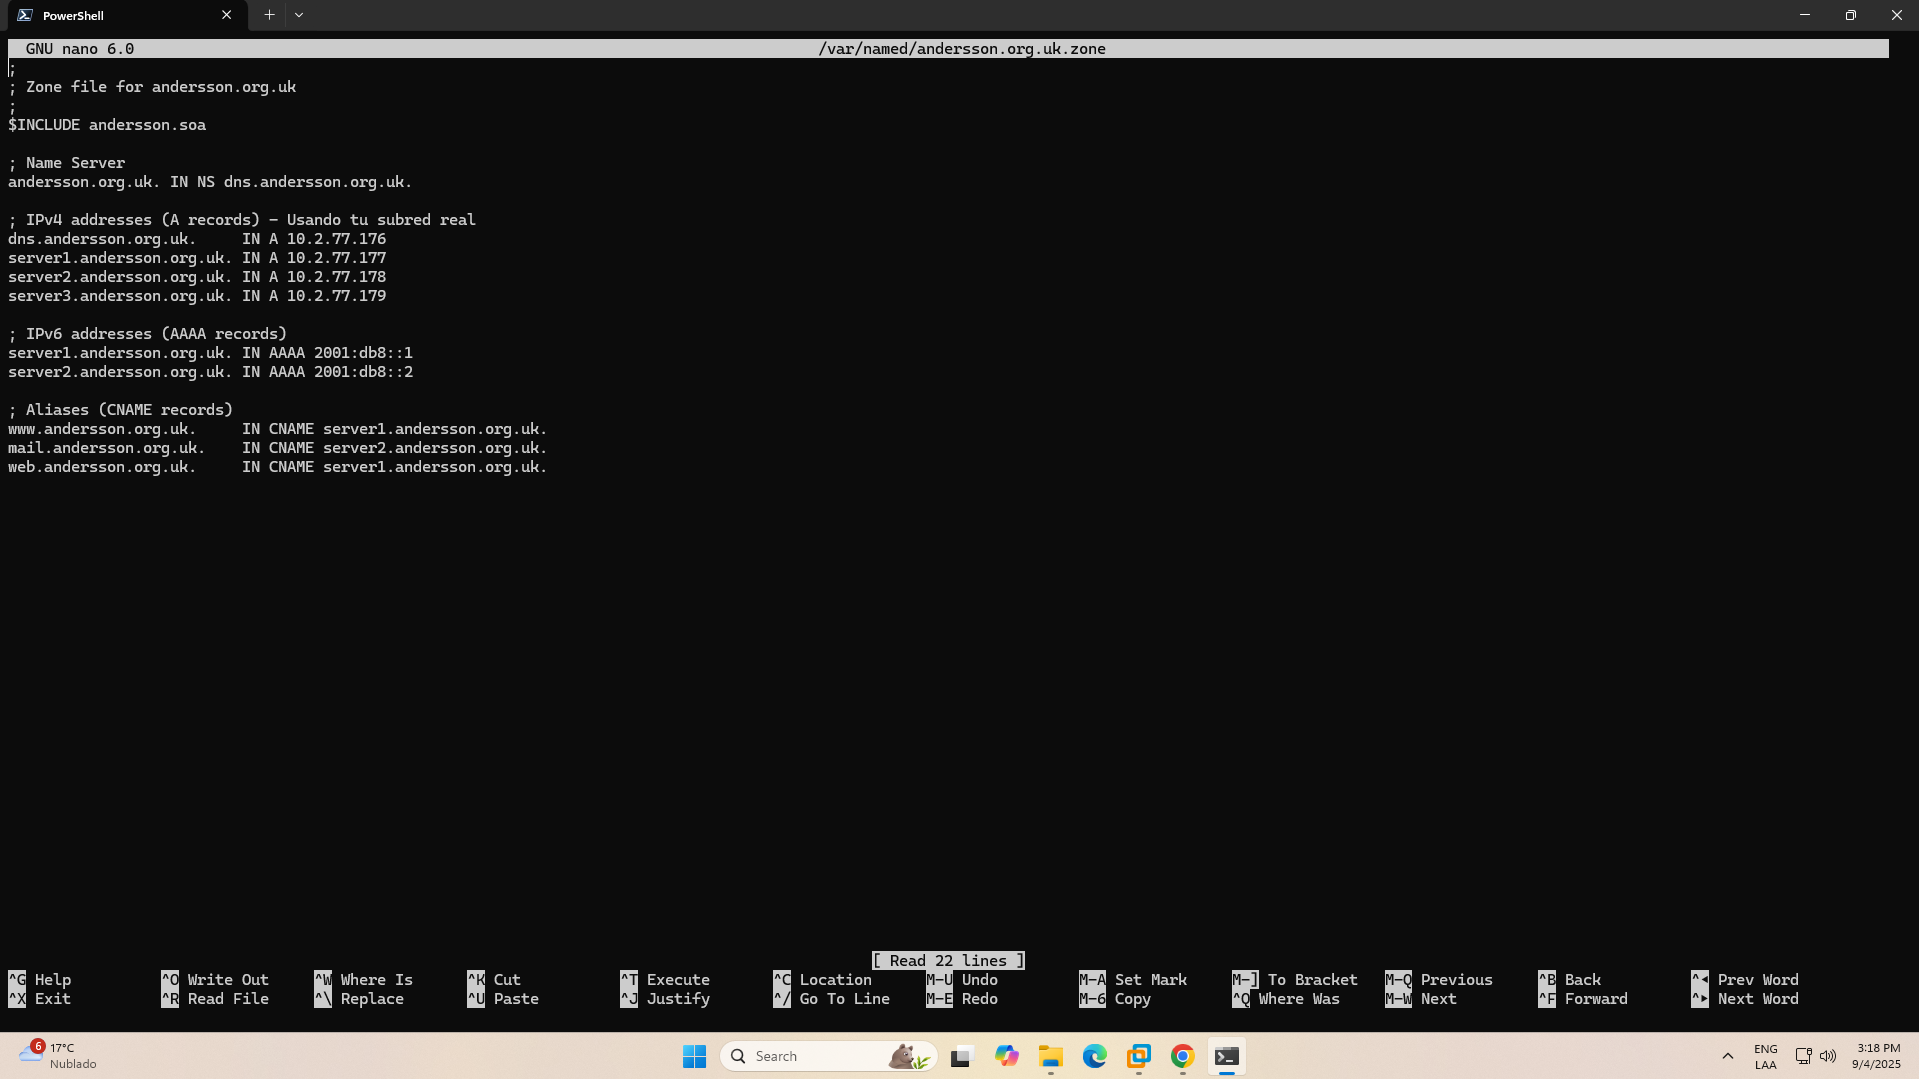
\includegraphics[keepaspectratio,alt={image.png}]{Third - DNS 263f56fc503e80ddb361c216e75fd3bf/image 3.png}}
\caption{image.png}
\end{figure}

\subsubsection{2.7 Start the DNS service🏗️}\label{start-the-dns-service}

\begin{Shaded}
\begin{Highlighting}[]
\ExtensionTok{/usr/sbin/named}
\end{Highlighting}
\end{Shaded}

\subsubsection{2.8 Check if it's running}\label{check-if-its-running}

\begin{Shaded}
\begin{Highlighting}[]

\FunctionTok{ps}\NormalTok{ aux }\KeywordTok{|} \FunctionTok{grep}\NormalTok{ named}
\FunctionTok{netstat} \AttributeTok{{-}ln} \KeywordTok{|} \FunctionTok{grep}\NormalTok{ :53}
\end{Highlighting}
\end{Shaded}

\begin{figure}
\centering
\pandocbounded{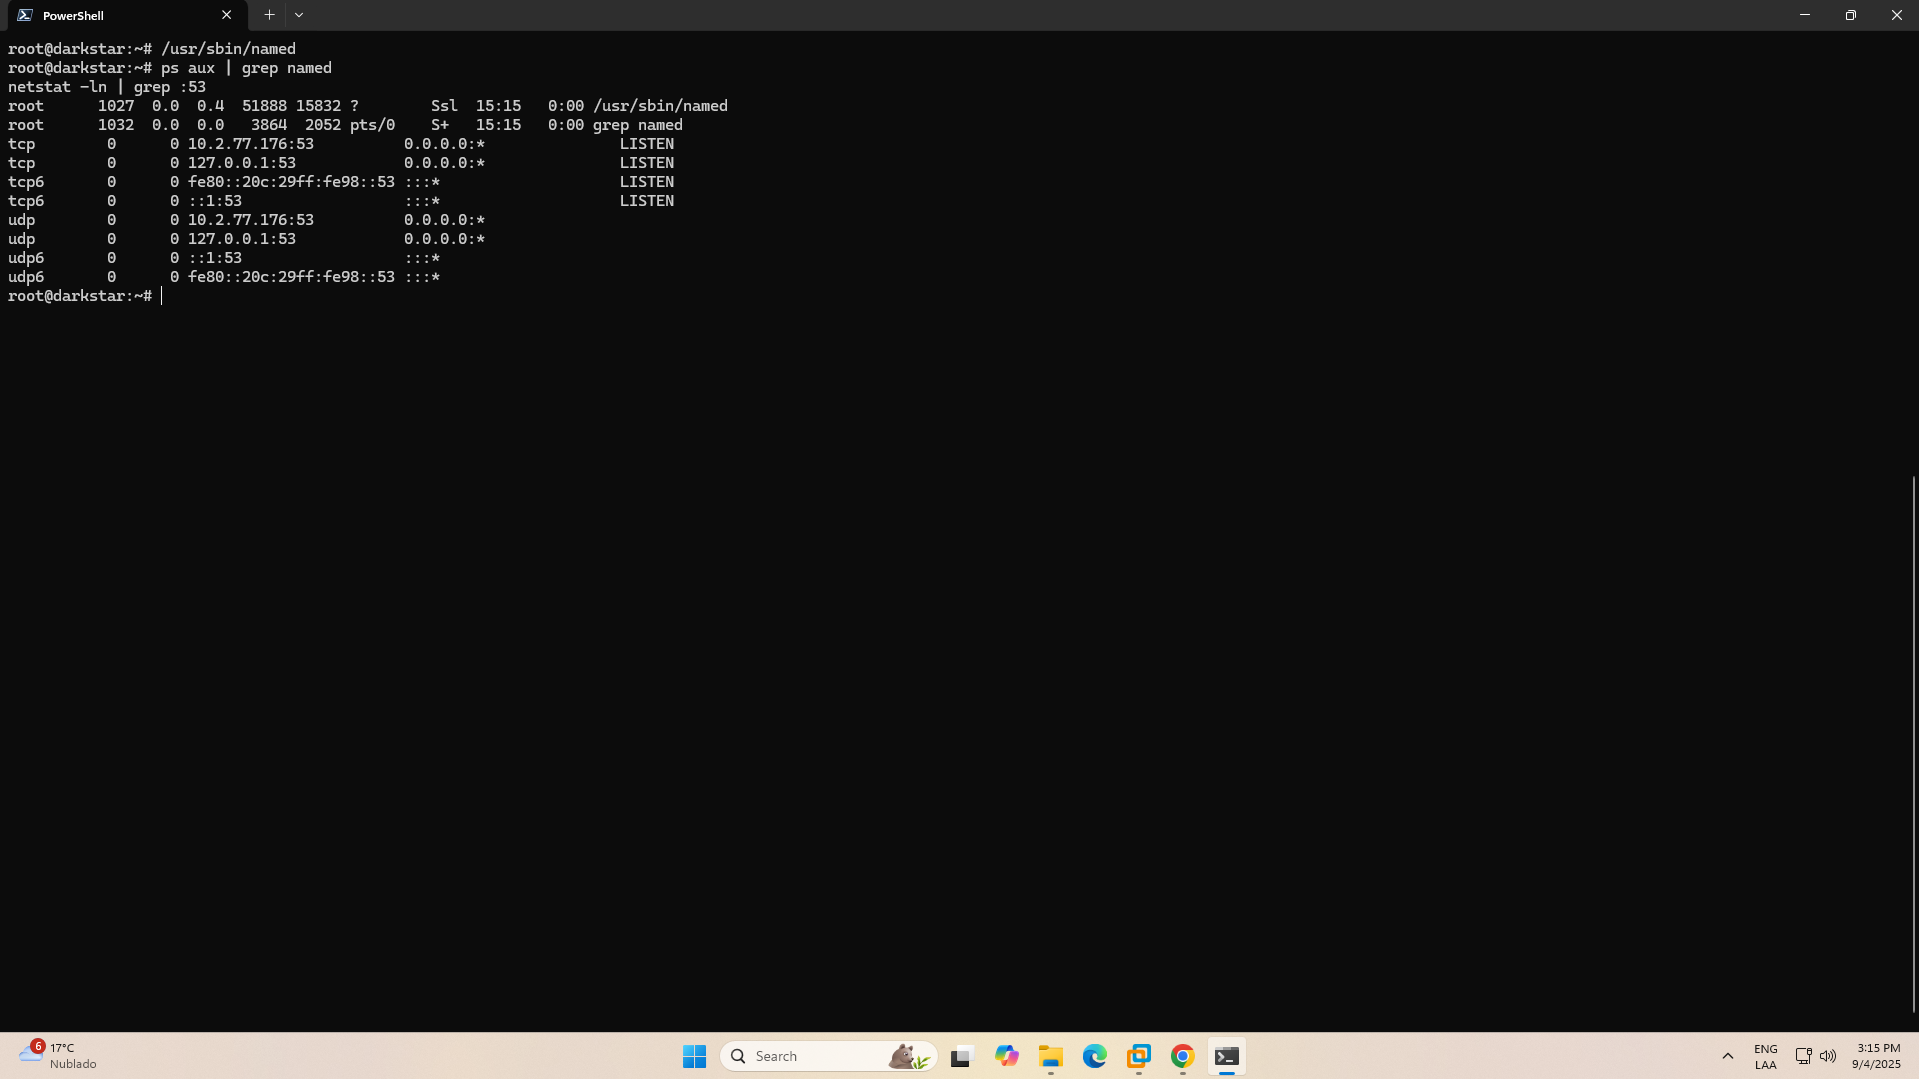
\includegraphics[keepaspectratio,alt={image.png}]{Third - DNS 263f56fc503e80ddb361c216e75fd3bf/image 4.png}}
\caption{image.png}
\end{figure}

\subsection{Step 3: Test Your Slackware DNS
Server}\label{step-3-test-your-slackware-dns-server}

\subsubsection{3.1 Configure the server to use itself as
DNS}\label{configure-the-server-to-use-itself-as-dns}

\begin{Shaded}
\begin{Highlighting}[]
\FunctionTok{nano}\NormalTok{ /etc/resolv.conf}
\end{Highlighting}
\end{Shaded}

Add:

\begin{Shaded}
\begin{Highlighting}[]
\ExtensionTok{nameserver}\NormalTok{ 127.0.0.1}
\ExtensionTok{nameserver}\NormalTok{ 192.168.1.10  }\CommentTok{\# Your DNS server IP}
\end{Highlighting}
\end{Shaded}

\begin{figure}
\centering
\pandocbounded{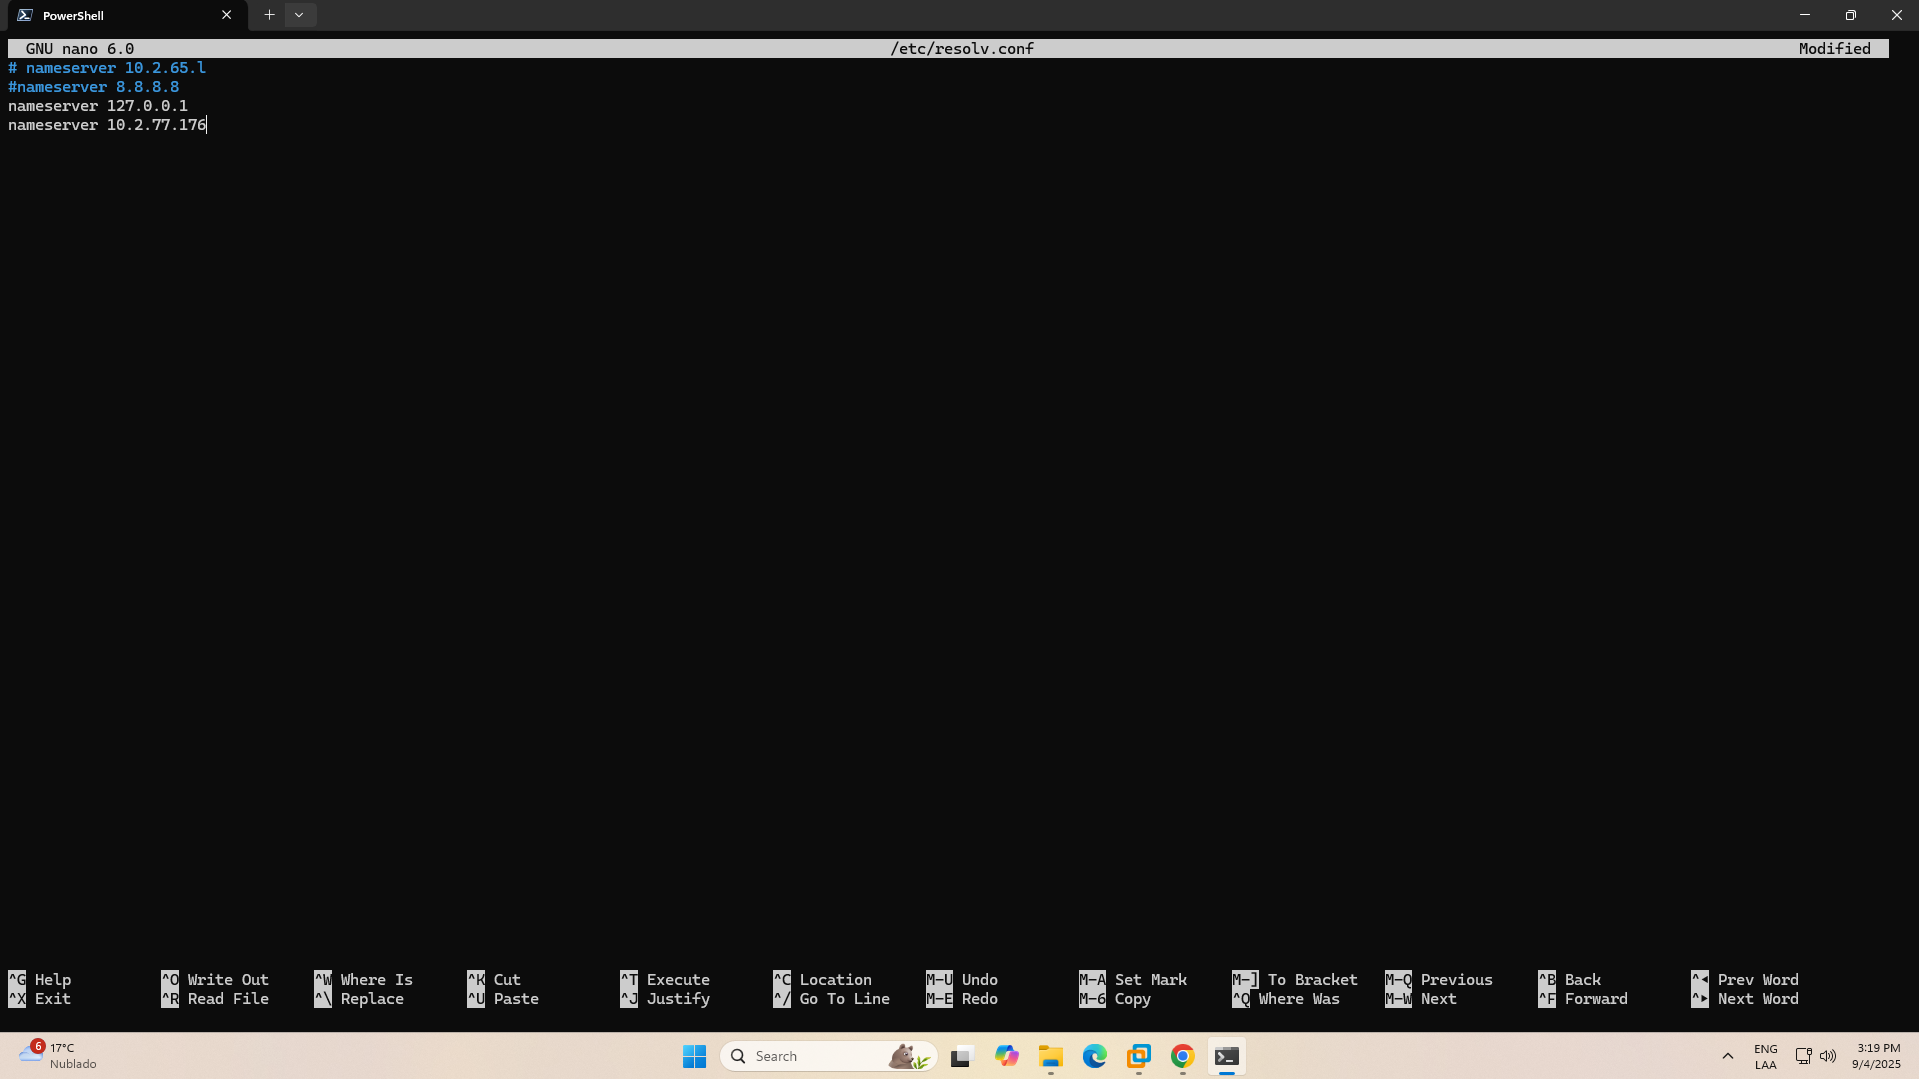
\includegraphics[keepaspectratio,alt={image.png}]{Third - DNS 263f56fc503e80ddb361c216e75fd3bf/image 5.png}}
\caption{image.png}
\end{figure}

\subsubsection{3.2 Test with nslookup}\label{test-with-nslookup}

\begin{Shaded}
\begin{Highlighting}[]
\ExtensionTok{nslookup}
\OperatorTok{\textgreater{}}\NormalTok{ server1.andersson.org.uk}
\OperatorTok{\textgreater{}}\NormalTok{ www.andersson.org.uk}
\OperatorTok{\textgreater{}}\NormalTok{ dns.andersson.org.uk}
\OperatorTok{\textgreater{}}\NormalTok{ www.google.com}
\OperatorTok{\textgreater{}}\NormalTok{ exit}
\end{Highlighting}
\end{Shaded}

\begin{figure}
\centering
\pandocbounded{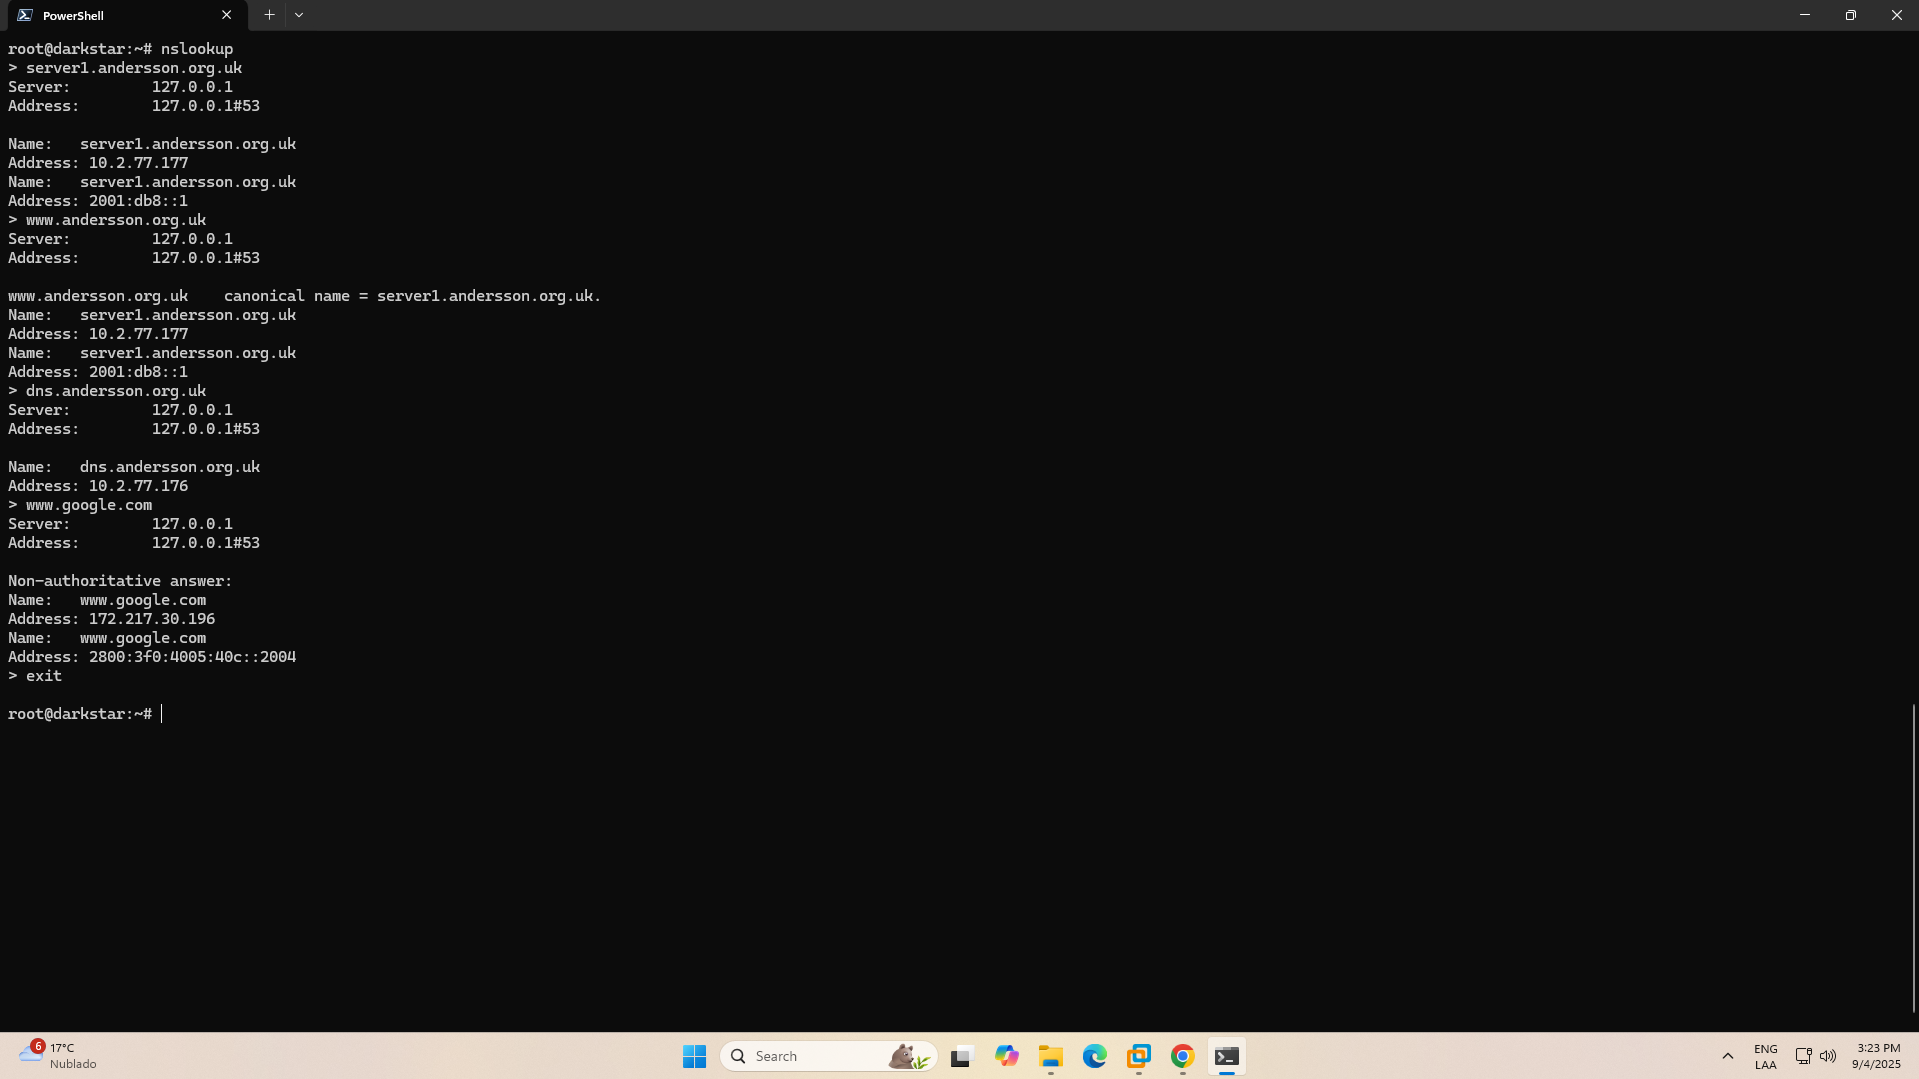
\includegraphics[keepaspectratio,alt={image.png}]{Third - DNS 263f56fc503e80ddb361c216e75fd3bf/image 6.png}}
\caption{image.png}
\end{figure}

\subsection{Before We Continue to
Solaris\ldots{}}\label{before-we-continue-to-solaris}

\textbf{Tell me:}

\begin{enumerate}
\def\labelenumi{\arabic{enumi}.}
\tightlist
\item
  What names did you choose for your domains? (Replace {[}yourname1{]}
  and {[}yourname2{]})
\item
  What IP address range were you assigned?
\item
  Did the Slackware DNS server start successfully?
\end{enumerate}

Once you confirm this works, we'll configure Solaris as the primary for
the first domain and then set up the secondary servers.

\textbf{Are you ready to test this first part?}

\begin{center}\rule{0.5\linewidth}{0.5pt}\end{center}

\subsection{Paso 3.3: Reiniciar el
servicio}\label{paso-3.3-reiniciar-el-servicio}

bash

\texttt{*killall\ named*\ */usr/sbin/named*}

\subsection{\texorpdfstring{\textbf{\emph{Make BIND Start Automatically
on
Boot}}}{Make BIND Start Automatically on Boot}}\label{make-bind-start-automatically-on-boot}

\subsection{Make BIND Start Automatically on
Boot}\label{make-bind-start-automatically-on-boot-1}

First, let's check if there's already a startup script:

\begin{Shaded}
\begin{Highlighting}[]
\FunctionTok{ls} \AttributeTok{{-}la}\NormalTok{ /etc/rc.d/rc.bind}\PreprocessorTok{*}
\end{Highlighting}
\end{Shaded}

If it exists, make it executable and enable it:

\begin{Shaded}
\begin{Highlighting}[]
\FunctionTok{chmod}\NormalTok{ +x /etc/rc.d/rc.bind}
\end{Highlighting}
\end{Shaded}

\begin{figure}
\centering
\pandocbounded{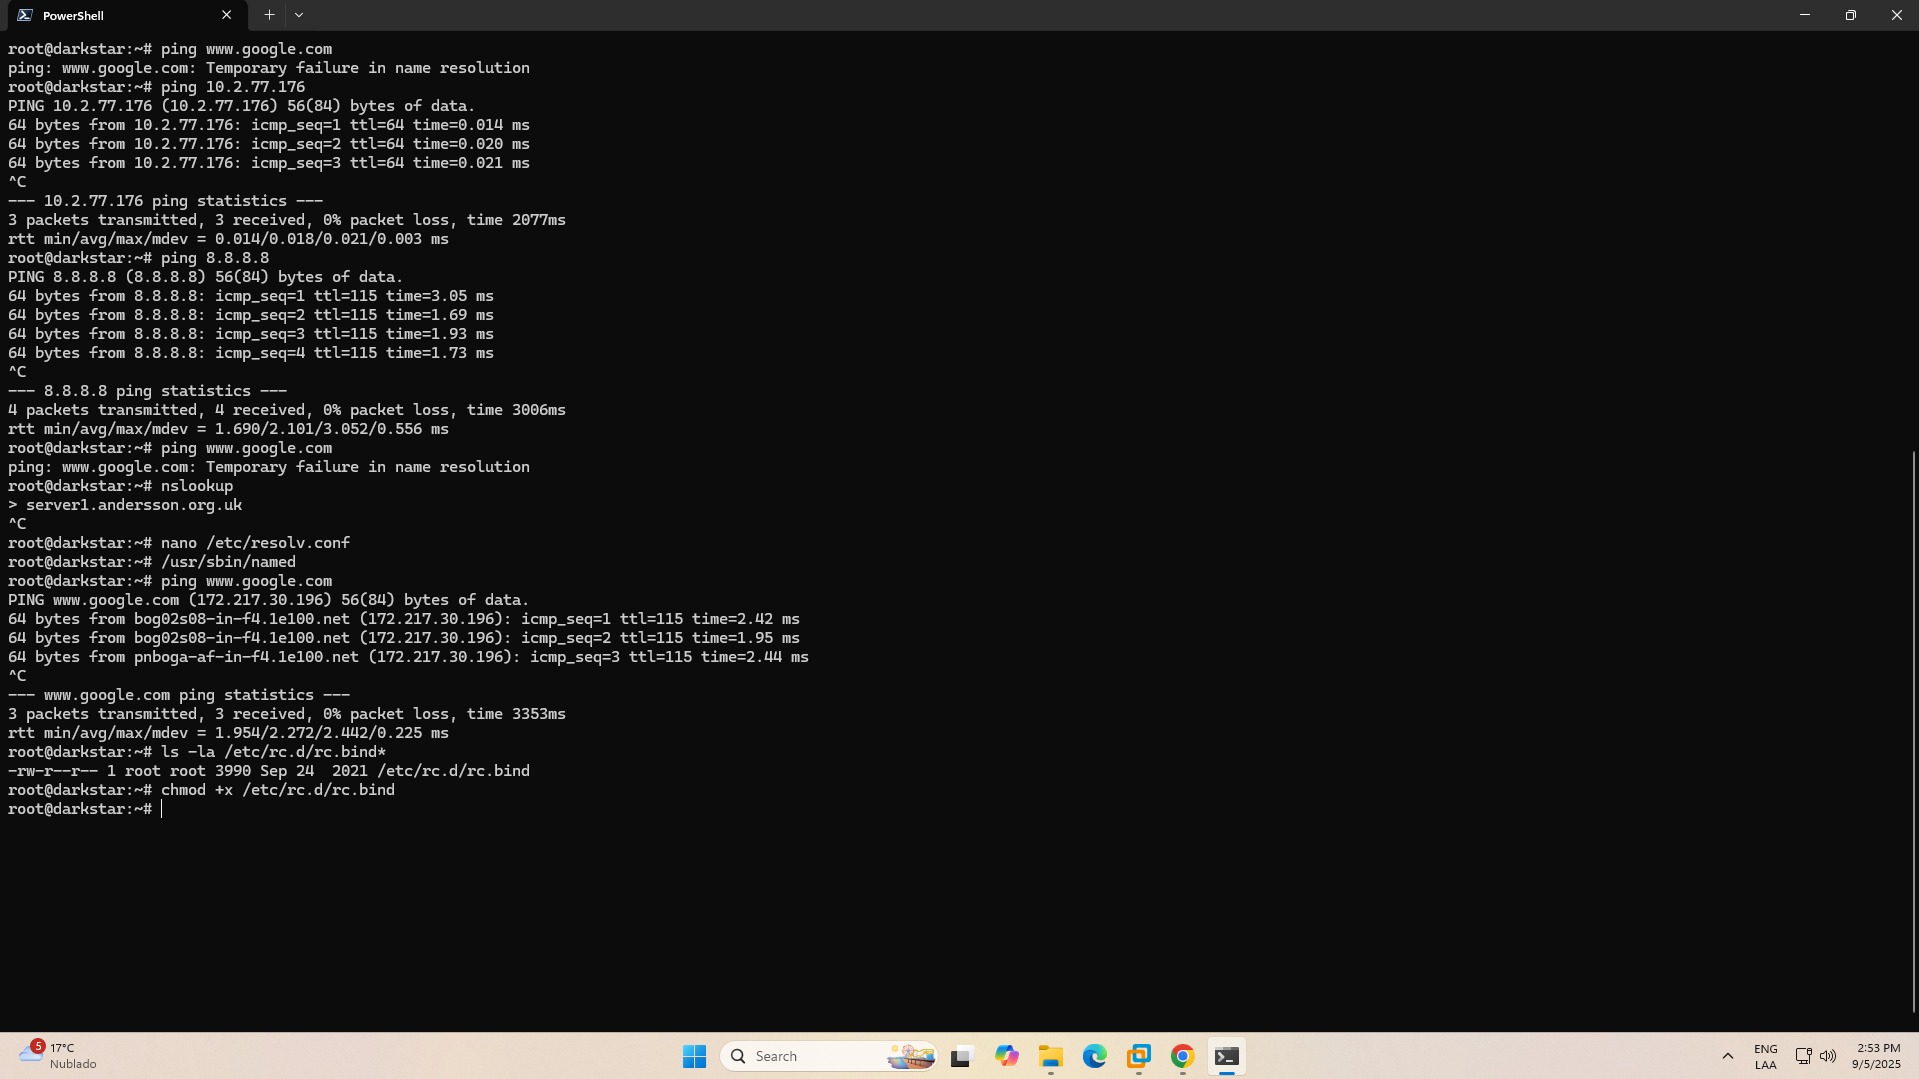
\includegraphics[keepaspectratio,alt={image.png}]{Third - DNS 263f56fc503e80ddb361c216e75fd3bf/image 7.png}}
\caption{image.png}
\end{figure}

O añadir a archivo de arranque

\section{SOLARIS - PRYMARY DNS ✅}\label{solaris---prymary-dns}

¡Perfecto! Ahora configuremos Solaris como servidor DNS primario para
\texttt{cristian.com.it}.

\subsection{Configuración Solaris DNS
Server}\label{configuraciuxf3n-solaris-dns-server}

\textbf{IP Solaris}: 10.2.77.178

\textbf{Gateway}: 10.2.65.1

\textbf{Dominio}: cristian.com.it (Primario)

\subsection{Paso 1: Verificar si BIND está
instalado}\label{paso-1-verificar-si-bind-estuxe1-instalado}

\begin{Shaded}
\begin{Highlighting}[]
\ExtensionTok{solaris\#}\NormalTok{ which named}
\ExtensionTok{solaris\#}\NormalTok{ ls /usr/sbin/named}
\end{Highlighting}
\end{Shaded}

\begin{figure}
\centering
\pandocbounded{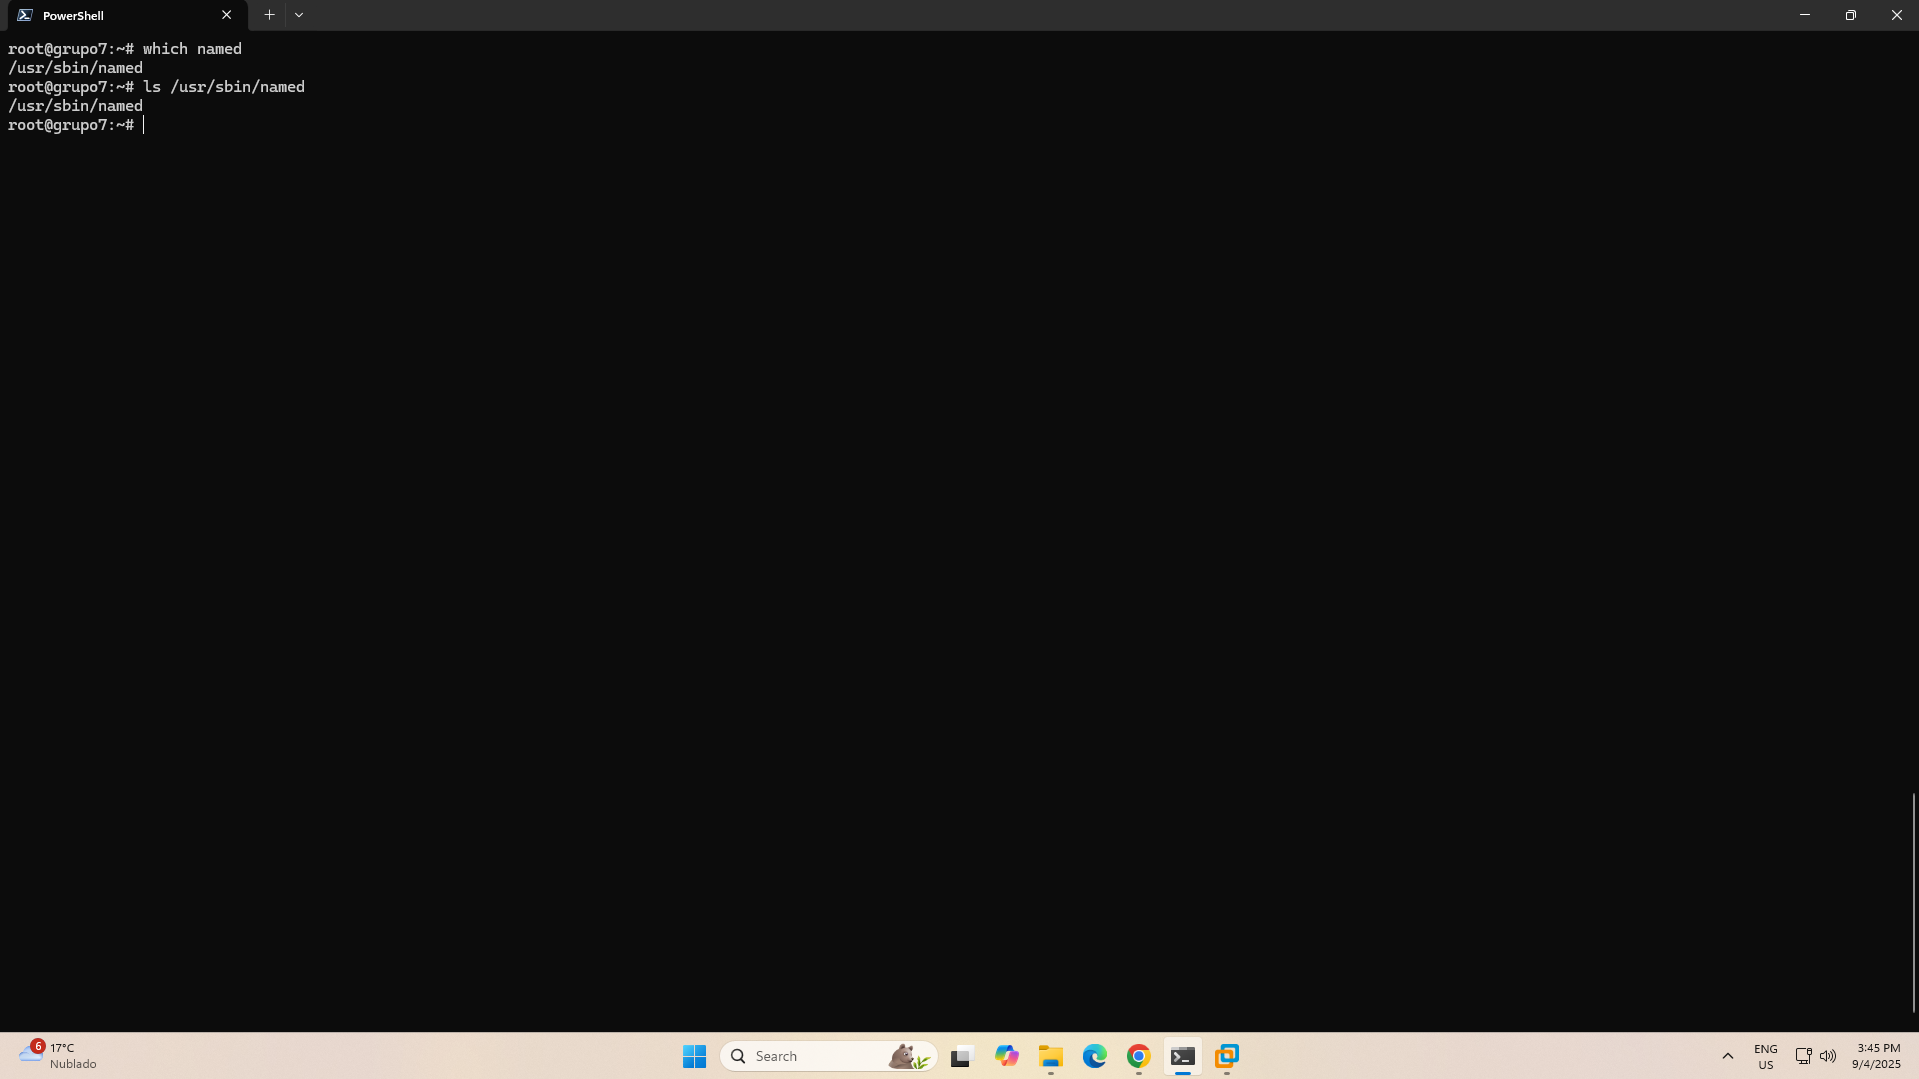
\includegraphics[keepaspectratio,alt={image.png}]{Third - DNS 263f56fc503e80ddb361c216e75fd3bf/image 8.png}}
\caption{image.png}
\end{figure}

Si no está instalado, instálalo desde los paquetes de Solaris.

\subsection{Paso 2: Crear la configuración
principal}\label{paso-2-crear-la-configuraciuxf3n-principal}

\begin{Shaded}
\begin{Highlighting}[]
\ExtensionTok{solaris\#}\NormalTok{ vi /etc/named.conf}
\end{Highlighting}
\end{Shaded}

\textbf{Contenido completo:}

\begin{Shaded}
\begin{Highlighting}[]
\ExtensionTok{options}\NormalTok{ \{}
        \ExtensionTok{directory} \StringTok{"/var/named"}\KeywordTok{;}
        \ExtensionTok{allow{-}query}\NormalTok{ \{ any}\KeywordTok{;} \ErrorTok{\}}\KeywordTok{;}
        \ExtensionTok{recursion}\NormalTok{ yes}\KeywordTok{;}
\ErrorTok{\}}\KeywordTok{;}

\ExtensionTok{//}\NormalTok{ Root zone}
\ExtensionTok{zone} \StringTok{"."}\NormalTok{ IN \{}
        \BuiltInTok{type}\NormalTok{ hint}\KeywordTok{;}
        \FunctionTok{file} \StringTok{"named.ca"}\KeywordTok{;}
\ErrorTok{\}}\KeywordTok{;}

\ExtensionTok{//}\NormalTok{ PRIMARY zone for cristian.com.it}
\ExtensionTok{zone} \StringTok{"cristian.com.it"}\NormalTok{ IN \{}
        \BuiltInTok{type}\NormalTok{ master}\KeywordTok{;}
        \FunctionTok{file} \StringTok{"cristian.com.it.zone"}\KeywordTok{;}
\ErrorTok{\}}\KeywordTok{;}

\ExtensionTok{//}\NormalTok{ SECONDARY zone for andersson.org.uk }\ErrorTok{(}\ExtensionTok{from}\NormalTok{ Slackware}\KeywordTok{)}
\ExtensionTok{zone} \StringTok{"andersson.org.uk"}\NormalTok{ IN \{}
        \BuiltInTok{type}\NormalTok{ slave}\KeywordTok{;}
        \FunctionTok{file} \StringTok{"andersson.org.uk.slave"}\KeywordTok{;}
        \ExtensionTok{masters}\NormalTok{ \{ 10.2.77.176}\KeywordTok{;} \ErrorTok{\}}\KeywordTok{;}
\ErrorTok{\}}\KeywordTok{;}

\ExtensionTok{//}\NormalTok{ Localhost zones}
\ExtensionTok{zone} \StringTok{"localhost"}\NormalTok{ IN \{}
        \BuiltInTok{type}\NormalTok{ master}\KeywordTok{;}
        \FunctionTok{file} \StringTok{"localhost.zone"}\KeywordTok{;}
        \ExtensionTok{allow{-}update}\NormalTok{ \{ none}\KeywordTok{;} \ErrorTok{\}}\KeywordTok{;}
\ErrorTok{\}}\KeywordTok{;}

\ExtensionTok{zone} \StringTok{"0.0.127.in{-}addr.arpa"}\NormalTok{ IN \{}
        \BuiltInTok{type}\NormalTok{ master}\KeywordTok{;}
        \FunctionTok{file} \StringTok{"named.local"}\KeywordTok{;}
        \ExtensionTok{allow{-}update}\NormalTok{ \{ none}\KeywordTok{;} \ErrorTok{\}}\KeywordTok{;}
\ErrorTok{\}}\KeywordTok{;}
\end{Highlighting}
\end{Shaded}

\begin{figure}
\centering
\pandocbounded{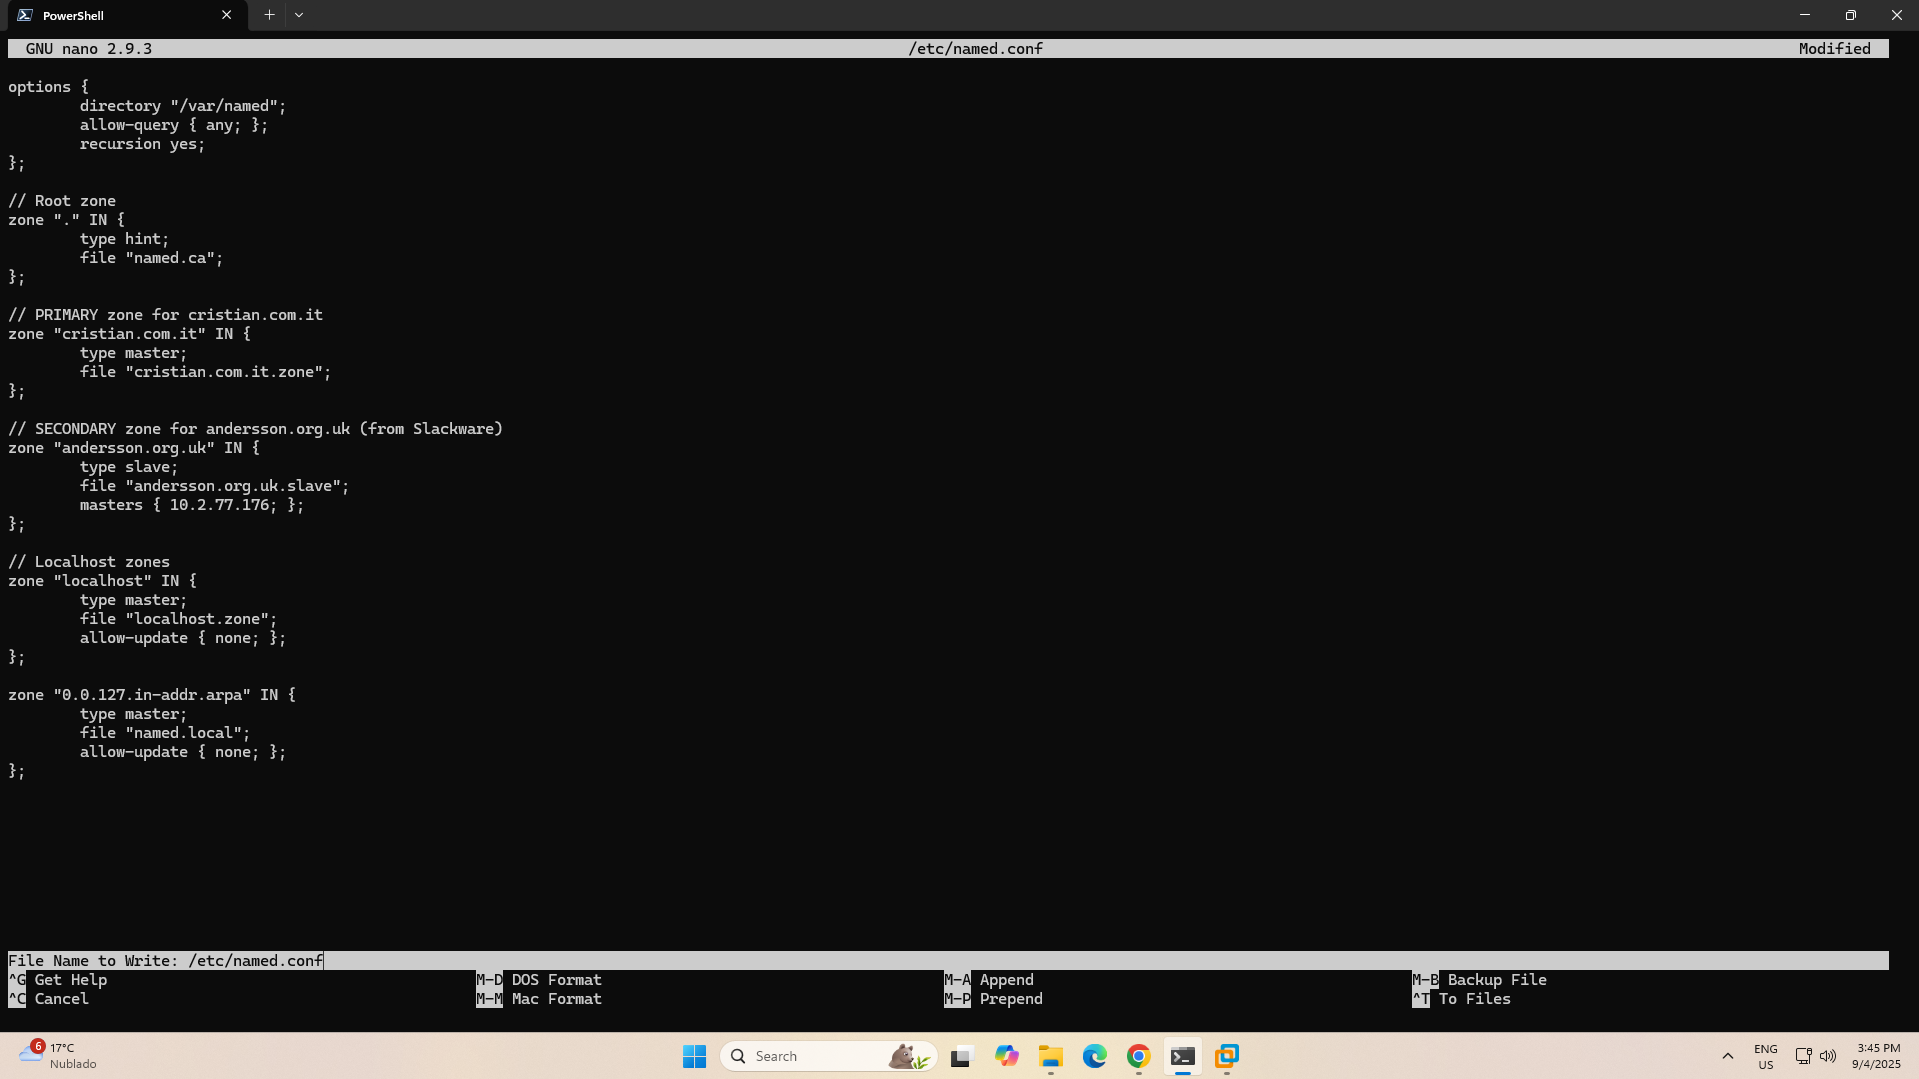
\includegraphics[keepaspectratio,alt={image.png}]{Third - DNS 263f56fc503e80ddb361c216e75fd3bf/image 9.png}}
\caption{image.png}
\end{figure}

\subsection{Paso 3: Crear directorio y archivos
básicos}\label{paso-3-crear-directorio-y-archivos-buxe1sicos}

\begin{Shaded}
\begin{Highlighting}[]
\ExtensionTok{solaris\#}\NormalTok{ mkdir }\AttributeTok{{-}p}\NormalTok{ /var/named}
\end{Highlighting}
\end{Shaded}

\subsubsection{Crear archivo de root
servers}\label{crear-archivo-de-root-servers}

\begin{Shaded}
\begin{Highlighting}[]
\ExtensionTok{solaris\#}\NormalTok{ nano /var/named/named.ca}
\end{Highlighting}
\end{Shaded}

\textbf{Contenido:}

\begin{Shaded}
\begin{Highlighting}[]
\KeywordTok{;}
\KeywordTok{;} \ExtensionTok{Root}\NormalTok{ name servers}
\KeywordTok{;}
\BuiltInTok{.}\NormalTok{ 3600000 IN NS A.ROOT{-}SERVERS.NET.}
\BuiltInTok{.}\NormalTok{ 3600000 IN NS B.ROOT{-}SERVERS.NET.}
\BuiltInTok{.}\NormalTok{ 3600000 IN NS C.ROOT{-}SERVERS.NET.}

\KeywordTok{;} \ExtensionTok{Root}\NormalTok{ name servers by address}
\ExtensionTok{A.ROOT{-}SERVERS.NET.}\NormalTok{ 3600000 IN A 198.41.0.4}
\ExtensionTok{B.ROOT{-}SERVERS.NET.}\NormalTok{ 3600000 IN A 199.9.14.201}
\ExtensionTok{C.ROOT{-}SERVERS.NET.}\NormalTok{ 3600000 IN A 192.33.4.12}
\end{Highlighting}
\end{Shaded}

\begin{figure}
\centering
\pandocbounded{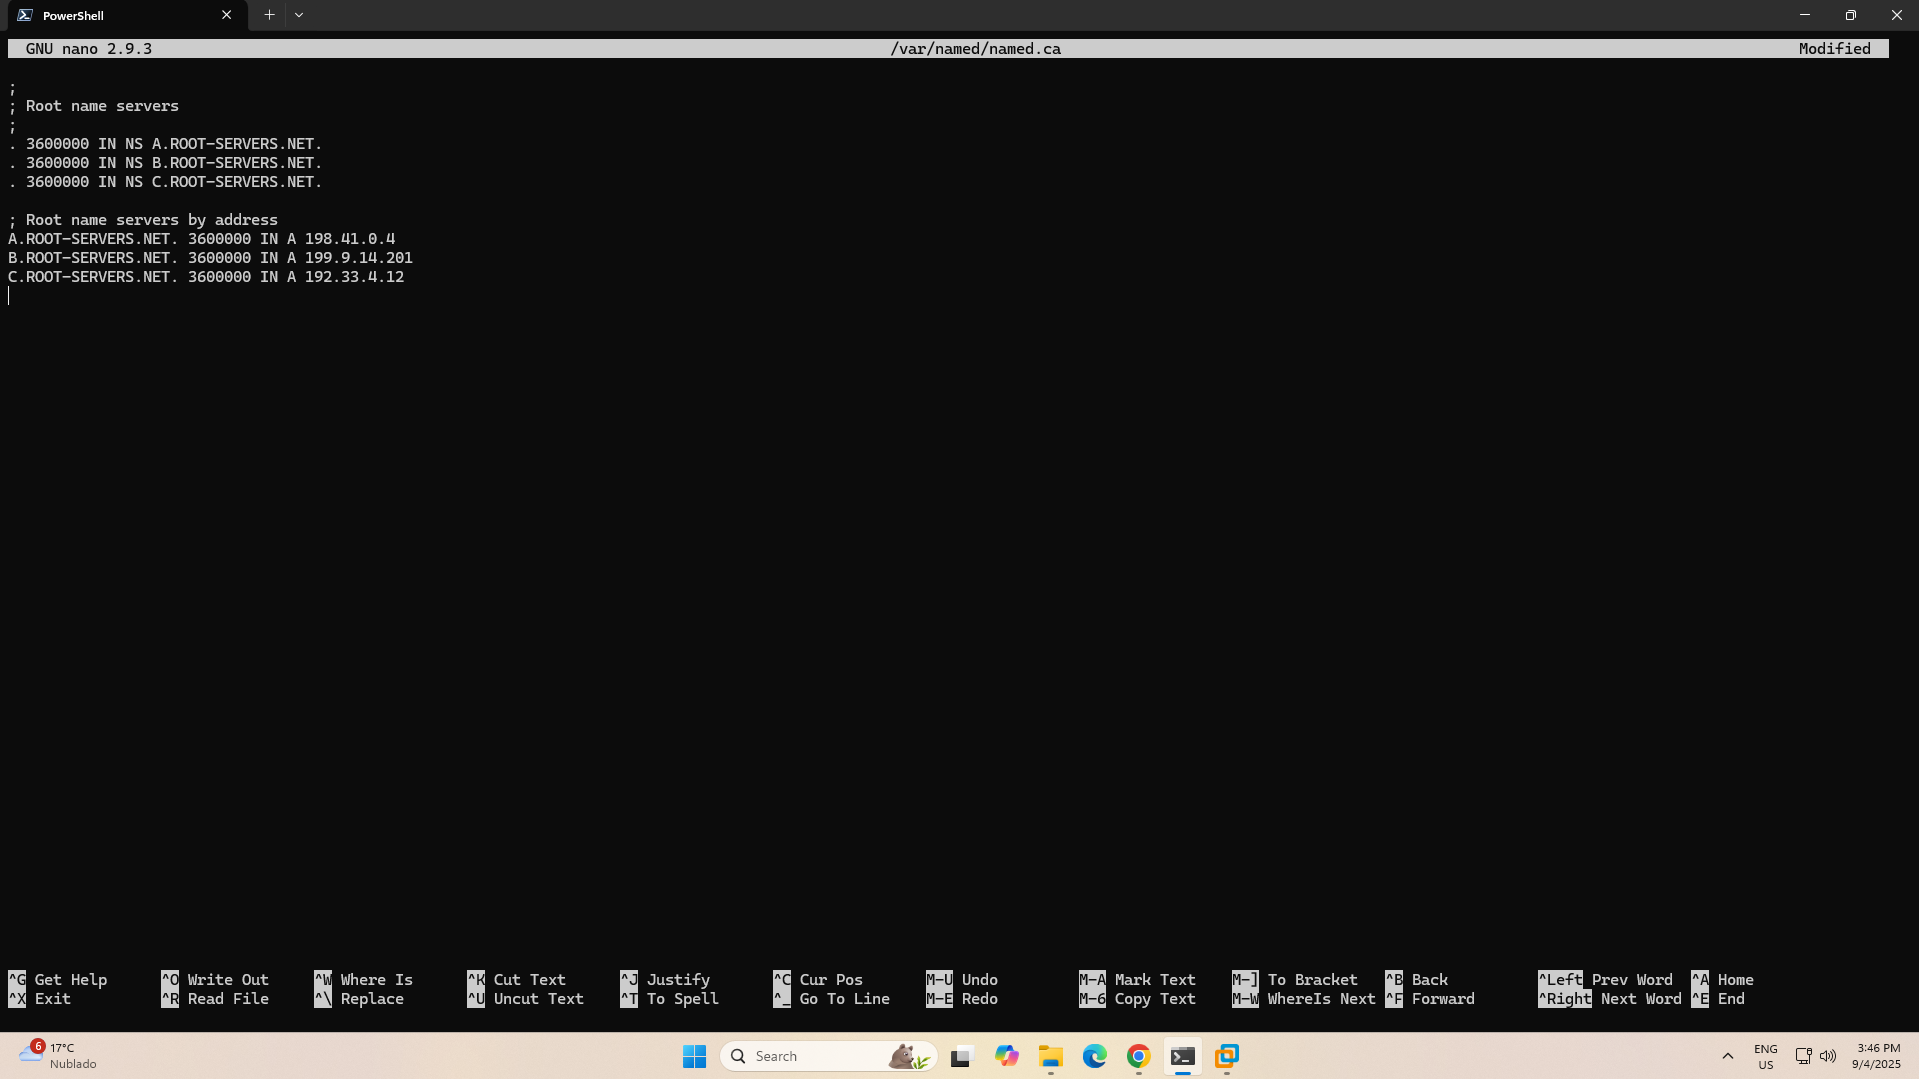
\includegraphics[keepaspectratio,alt={image.png}]{Third - DNS 263f56fc503e80ddb361c216e75fd3bf/image 10.png}}
\caption{image.png}
\end{figure}

\subsection{Paso 4: Crear archivo SOA}\label{paso-4-crear-archivo-soa}

\begin{Shaded}
\begin{Highlighting}[]
\ExtensionTok{solaris\#}\NormalTok{ vi /var/named/cristian.soa}
\end{Highlighting}
\end{Shaded}

\textbf{Contenido:}

\begin{Shaded}
\begin{Highlighting}[]
\KeywordTok{;}
\KeywordTok{;} \ExtensionTok{SOA}\NormalTok{ record for cristian.com.it}
\KeywordTok{;}
\ExtensionTok{@}\NormalTok{ IN SOA dns.cristian.com.it. admin.cristian.com.it. }\ErrorTok{(}
    \ExtensionTok{2024120401}  \KeywordTok{;} \ExtensionTok{Serial} \ErrorTok{(}\ExtensionTok{YYYYMMDDXX}\KeywordTok{)}
    \ExtensionTok{3600}        \KeywordTok{;} \ExtensionTok{Refresh} \ErrorTok{(}\ExtensionTok{1}\NormalTok{ hour}\KeywordTok{)}
    \ExtensionTok{1800}        \KeywordTok{;} \ExtensionTok{Retry} \ErrorTok{(}\ExtensionTok{30}\NormalTok{ minutes}\KeywordTok{)}
    \ExtensionTok{604800}      \KeywordTok{;} \ExtensionTok{Expire} \ErrorTok{(}\ExtensionTok{1}\NormalTok{ week}\KeywordTok{)}
    \ExtensionTok{86400}       \KeywordTok{;} \ExtensionTok{Minimum}\NormalTok{ TTL }\ErrorTok{(}\ExtensionTok{1}\NormalTok{ day}\KeywordTok{)}
\KeywordTok{)}
\end{Highlighting}
\end{Shaded}

\begin{figure}
\centering
\pandocbounded{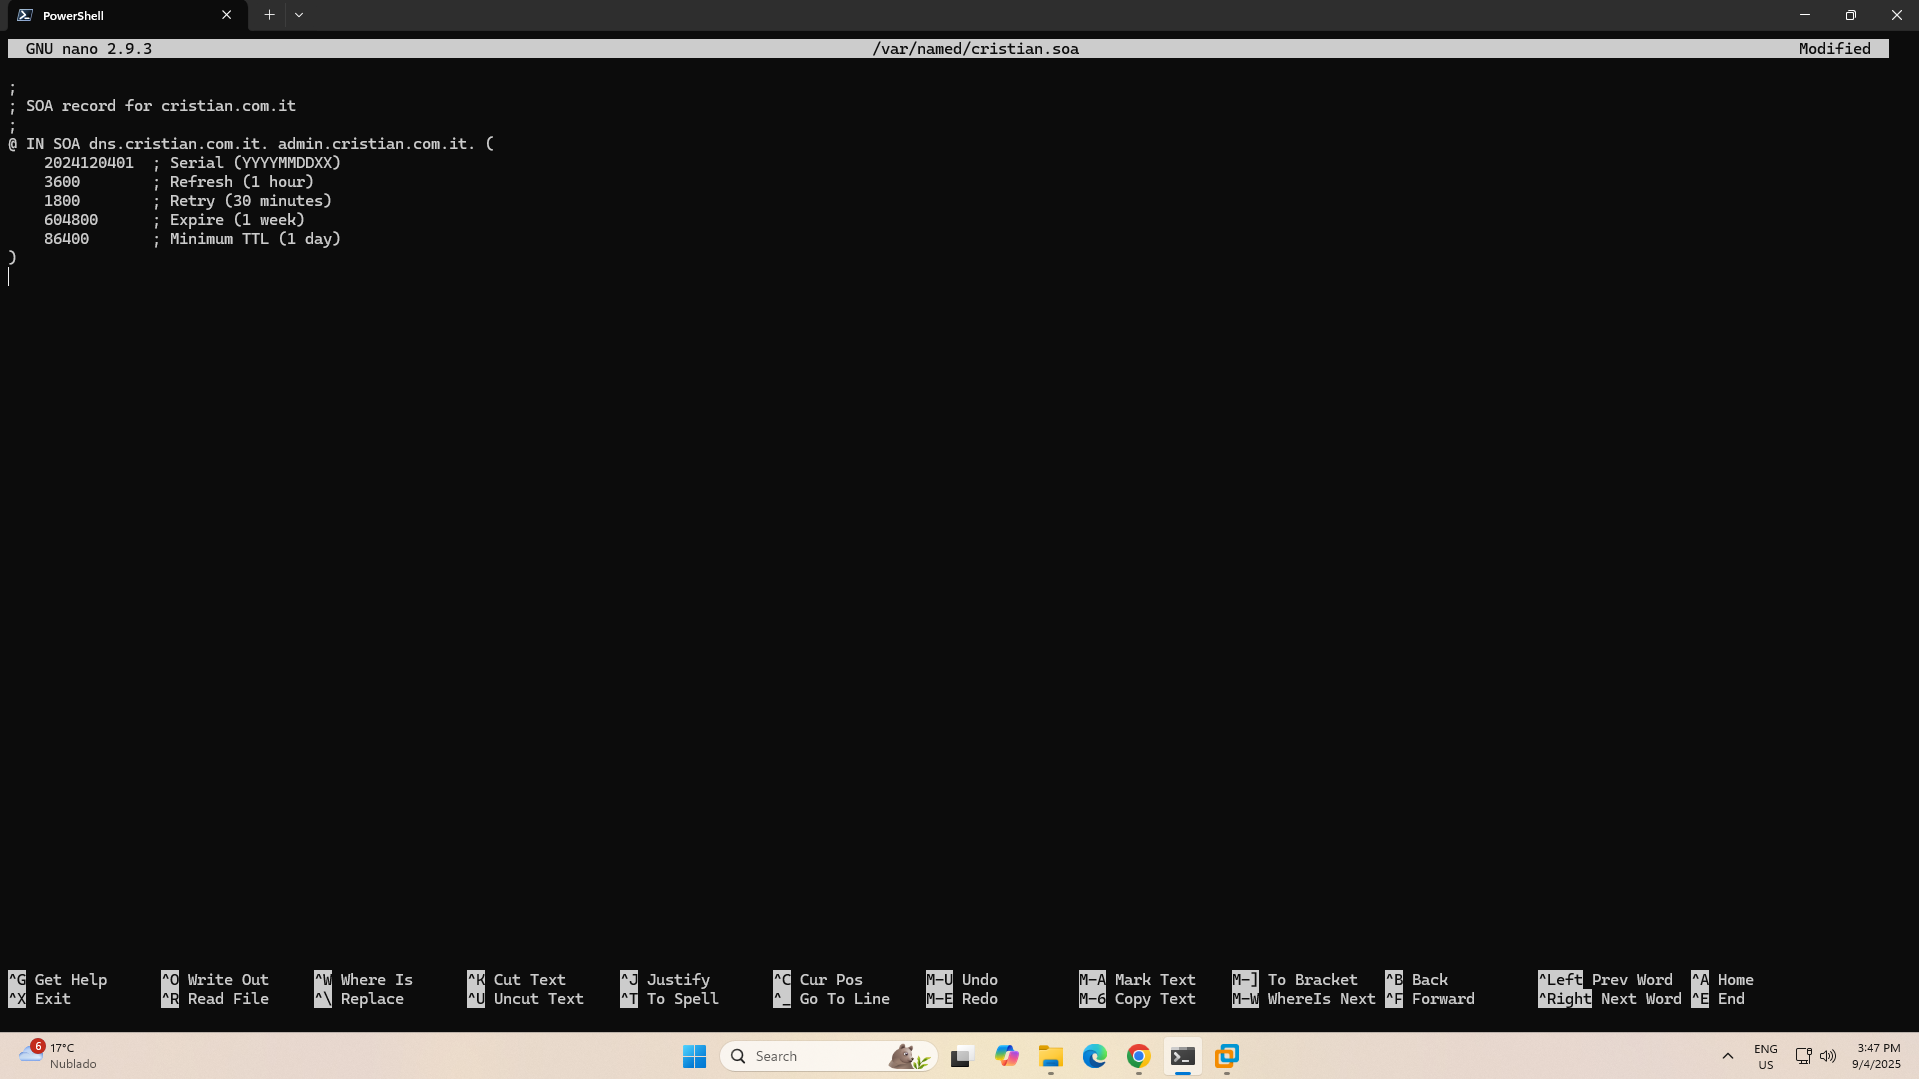
\includegraphics[keepaspectratio,alt={image.png}]{Third - DNS 263f56fc503e80ddb361c216e75fd3bf/image 11.png}}
\caption{image.png}
\end{figure}

\subsection{Paso 5: Crear archivo de zona
principal}\label{paso-5-crear-archivo-de-zona-principal}

\begin{Shaded}
\begin{Highlighting}[]
\ExtensionTok{solaris\#}\NormalTok{ nano /var/named/cristian.com.it.zone}
\end{Highlighting}
\end{Shaded}

\textbf{Contenido:}

\begin{Shaded}
\begin{Highlighting}[]
\KeywordTok{;}
\KeywordTok{;} \ExtensionTok{Zone}\NormalTok{ file for cristian.com.it}
\KeywordTok{;}
\VariableTok{$INCLUDE}\NormalTok{ /var/named/cristian.soa}

\KeywordTok{;} \ExtensionTok{Name}\NormalTok{ Server}
\ExtensionTok{cristian.com.it.}\NormalTok{ 86400 IN NS dns.cristian.com.it.}

\KeywordTok{;} \ExtensionTok{IPv4}\NormalTok{ addresses }\ErrorTok{(}\ExtensionTok{A}\NormalTok{ records}\KeywordTok{)} \ExtensionTok{{-}}\NormalTok{ Con TTL}
\ExtensionTok{dns.cristian.com.it.}\NormalTok{     86400 IN A 10.2.77.178}
\ExtensionTok{server1.cristian.com.it.}\NormalTok{ 86400 IN A 10.2.77.180}
\ExtensionTok{server2.cristian.com.it.}\NormalTok{ 86400 IN A 10.2.77.181}
\ExtensionTok{server3.cristian.com.it.}\NormalTok{ 86400 IN A 10.2.77.182}

\KeywordTok{;} \ExtensionTok{IPv6}\NormalTok{ addresses }\ErrorTok{(}\ExtensionTok{AAAA}\NormalTok{ records}\KeywordTok{)} \ExtensionTok{{-}}\NormalTok{ Con TTL}
\ExtensionTok{server1.cristian.com.it.}\NormalTok{ 86400 IN AAAA 2001:db8:1::1}
\ExtensionTok{server2.cristian.com.it.}\NormalTok{ 86400 IN AAAA 2001:db8:1::2}

\KeywordTok{;} \ExtensionTok{Aliases} \ErrorTok{(}\ExtensionTok{CNAME}\NormalTok{ records}\KeywordTok{)} \ExtensionTok{{-}}\NormalTok{ Con TTL}
\ExtensionTok{www.cristian.com.it.}\NormalTok{     86400 IN CNAME server1.cristian.com.it.}
\ExtensionTok{mail.cristian.com.it.}\NormalTok{    86400 IN CNAME server2.cristian.com.it.}
\ExtensionTok{web.cristian.com.it.}\NormalTok{     86400 IN CNAME server1.cristian.com.it.}
\end{Highlighting}
\end{Shaded}

\begin{figure}
\centering
\pandocbounded{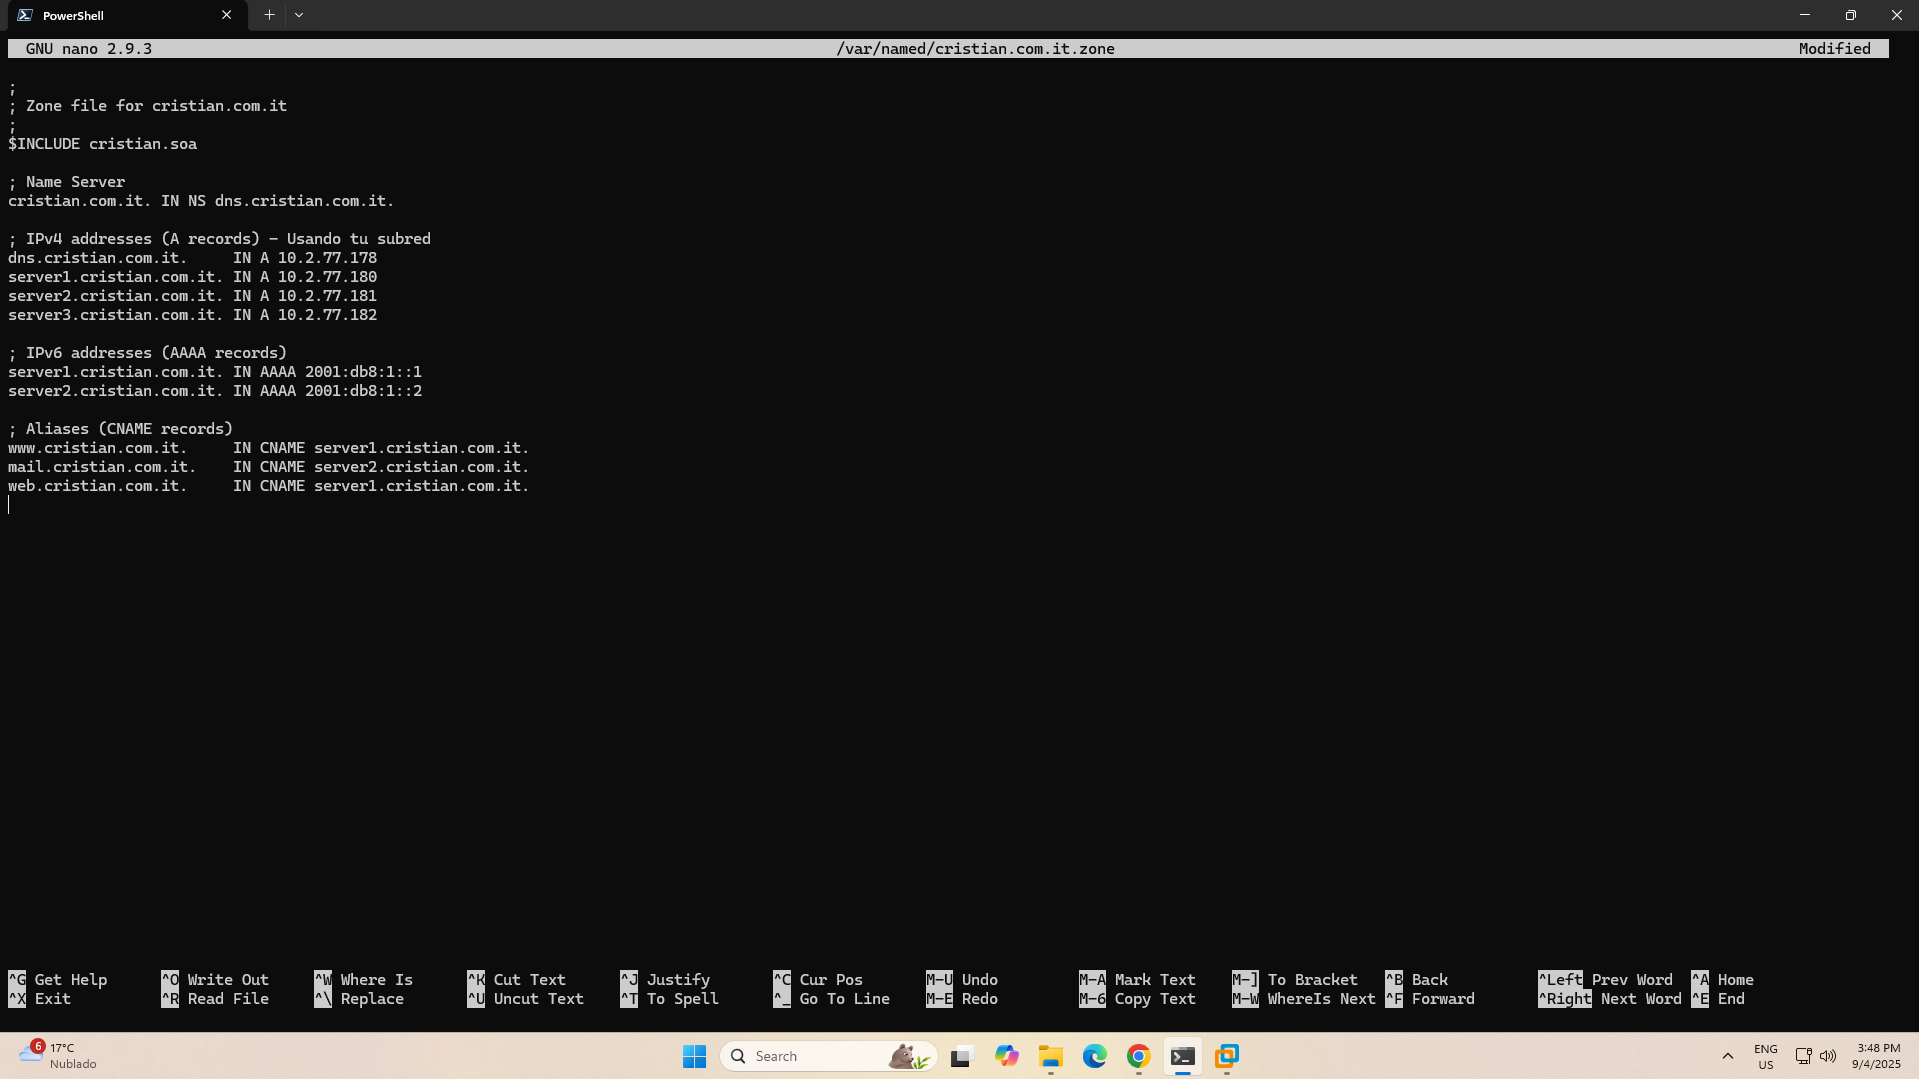
\includegraphics[keepaspectratio,alt={image.png}]{Third - DNS 263f56fc503e80ddb361c216e75fd3bf/image 12.png}}
\caption{image.png}
\end{figure}

\subsection{Paso 6: Crear archivos
localhost}\label{paso-6-crear-archivos-localhost}

\begin{Shaded}
\begin{Highlighting}[]
\ExtensionTok{solaris\#}\NormalTok{ nano /var/named/localhost.zone}
\end{Highlighting}
\end{Shaded}

\textbf{Contenido:}

\begin{Shaded}
\begin{Highlighting}[]
\ExtensionTok{@}\NormalTok{ IN SOA dns.cristian.com.it. admin.cristian.com.it. }\ErrorTok{(}
    \ExtensionTok{2024120401}
    \ExtensionTok{3600}
    \ExtensionTok{1800}
    \ExtensionTok{604800}
    \ExtensionTok{86400}
\KeywordTok{)}

\ExtensionTok{@}\NormalTok{ IN NS dns.cristian.com.it.}
\ExtensionTok{localhost}\NormalTok{ IN A 127.0.0.1}
\end{Highlighting}
\end{Shaded}

\begin{figure}
\centering
\pandocbounded{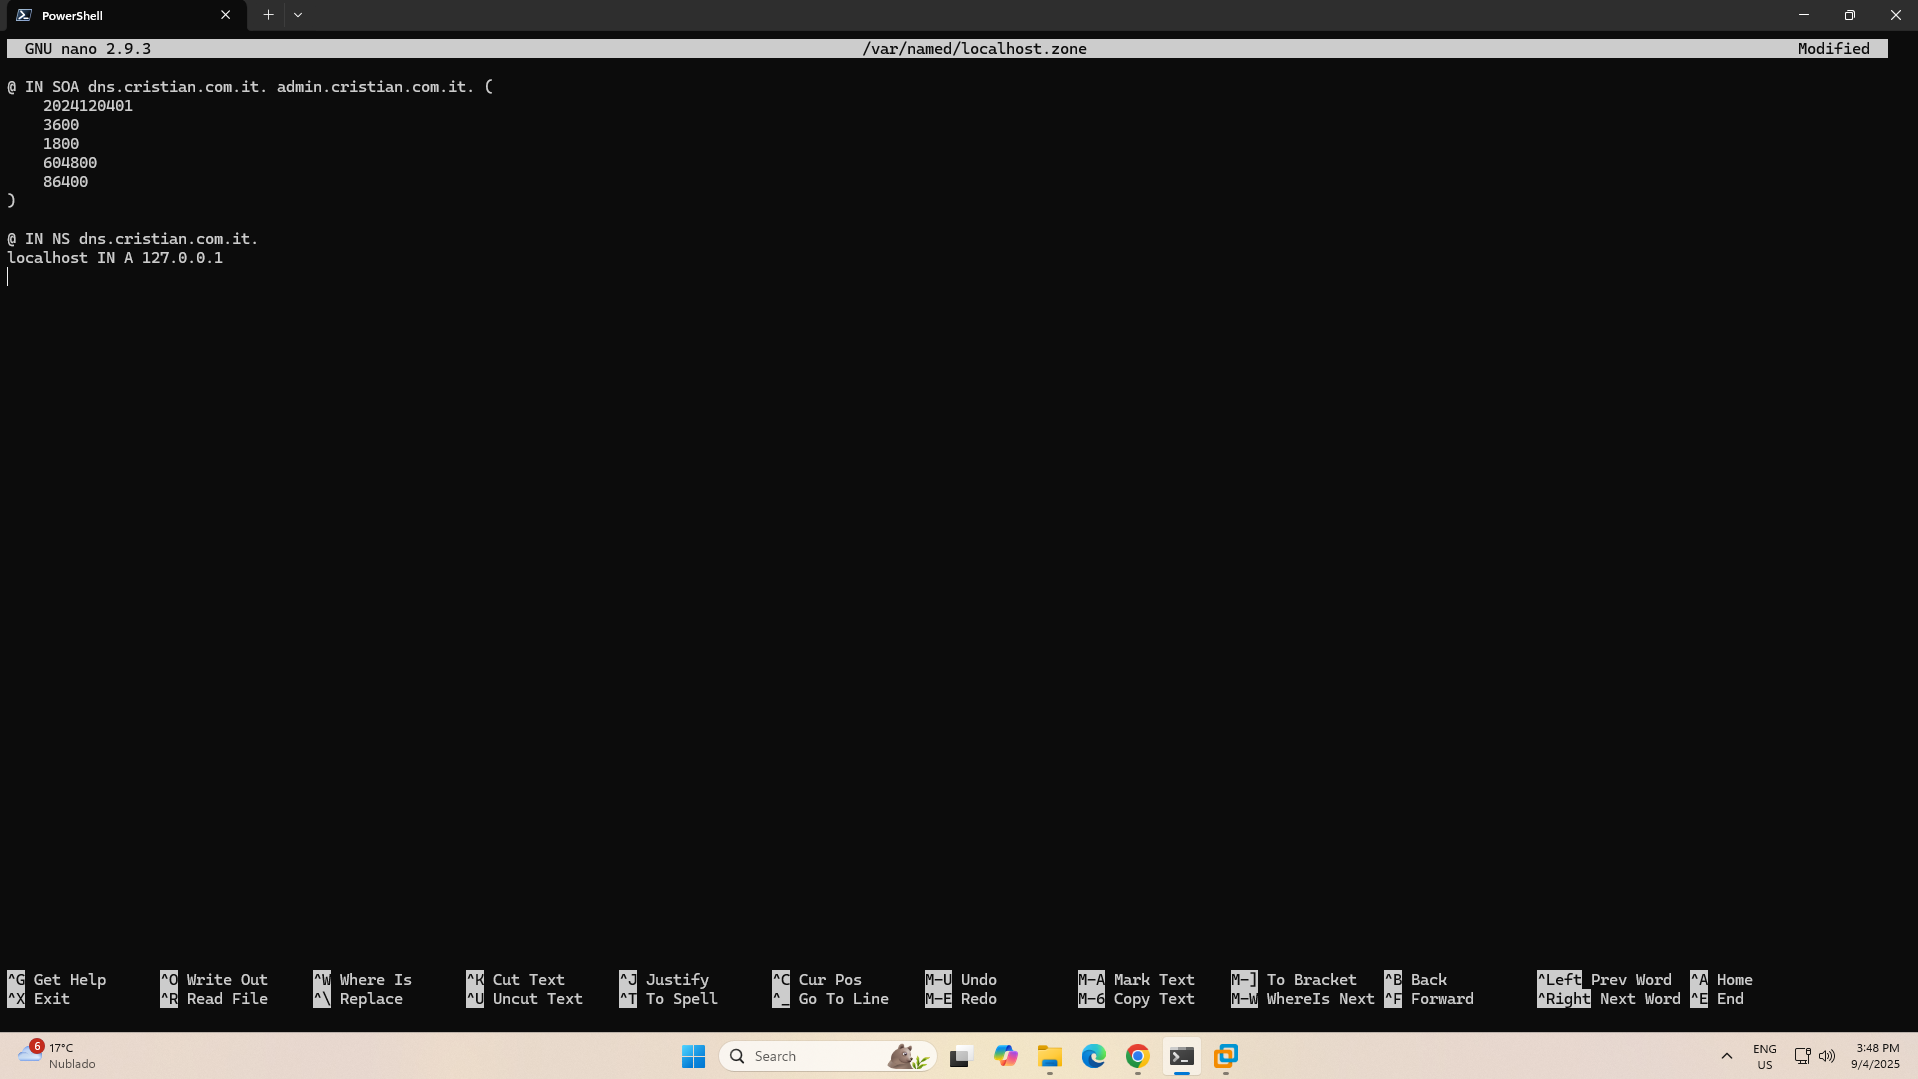
\includegraphics[keepaspectratio,alt={image.png}]{Third - DNS 263f56fc503e80ddb361c216e75fd3bf/image 13.png}}
\caption{image.png}
\end{figure}

\begin{Shaded}
\begin{Highlighting}[]
\ExtensionTok{solaris\#}\NormalTok{ nano /var/named/named.local}
\end{Highlighting}
\end{Shaded}

\textbf{Contenido:}

\begin{Shaded}
\begin{Highlighting}[]
\ExtensionTok{@}\NormalTok{ IN SOA dns.cristian.com.it. admin.cristian.com.it. }\ErrorTok{(}
    \ExtensionTok{2024120401}
    \ExtensionTok{3600}
    \ExtensionTok{1800}
    \ExtensionTok{604800}
    \ExtensionTok{86400}
\KeywordTok{)}

\ExtensionTok{@}\NormalTok{ IN NS dns.cristian.com.it.}
\ExtensionTok{1}\NormalTok{ IN PTR localhost.cristian.com.it.}
\end{Highlighting}
\end{Shaded}

\begin{figure}
\centering
\pandocbounded{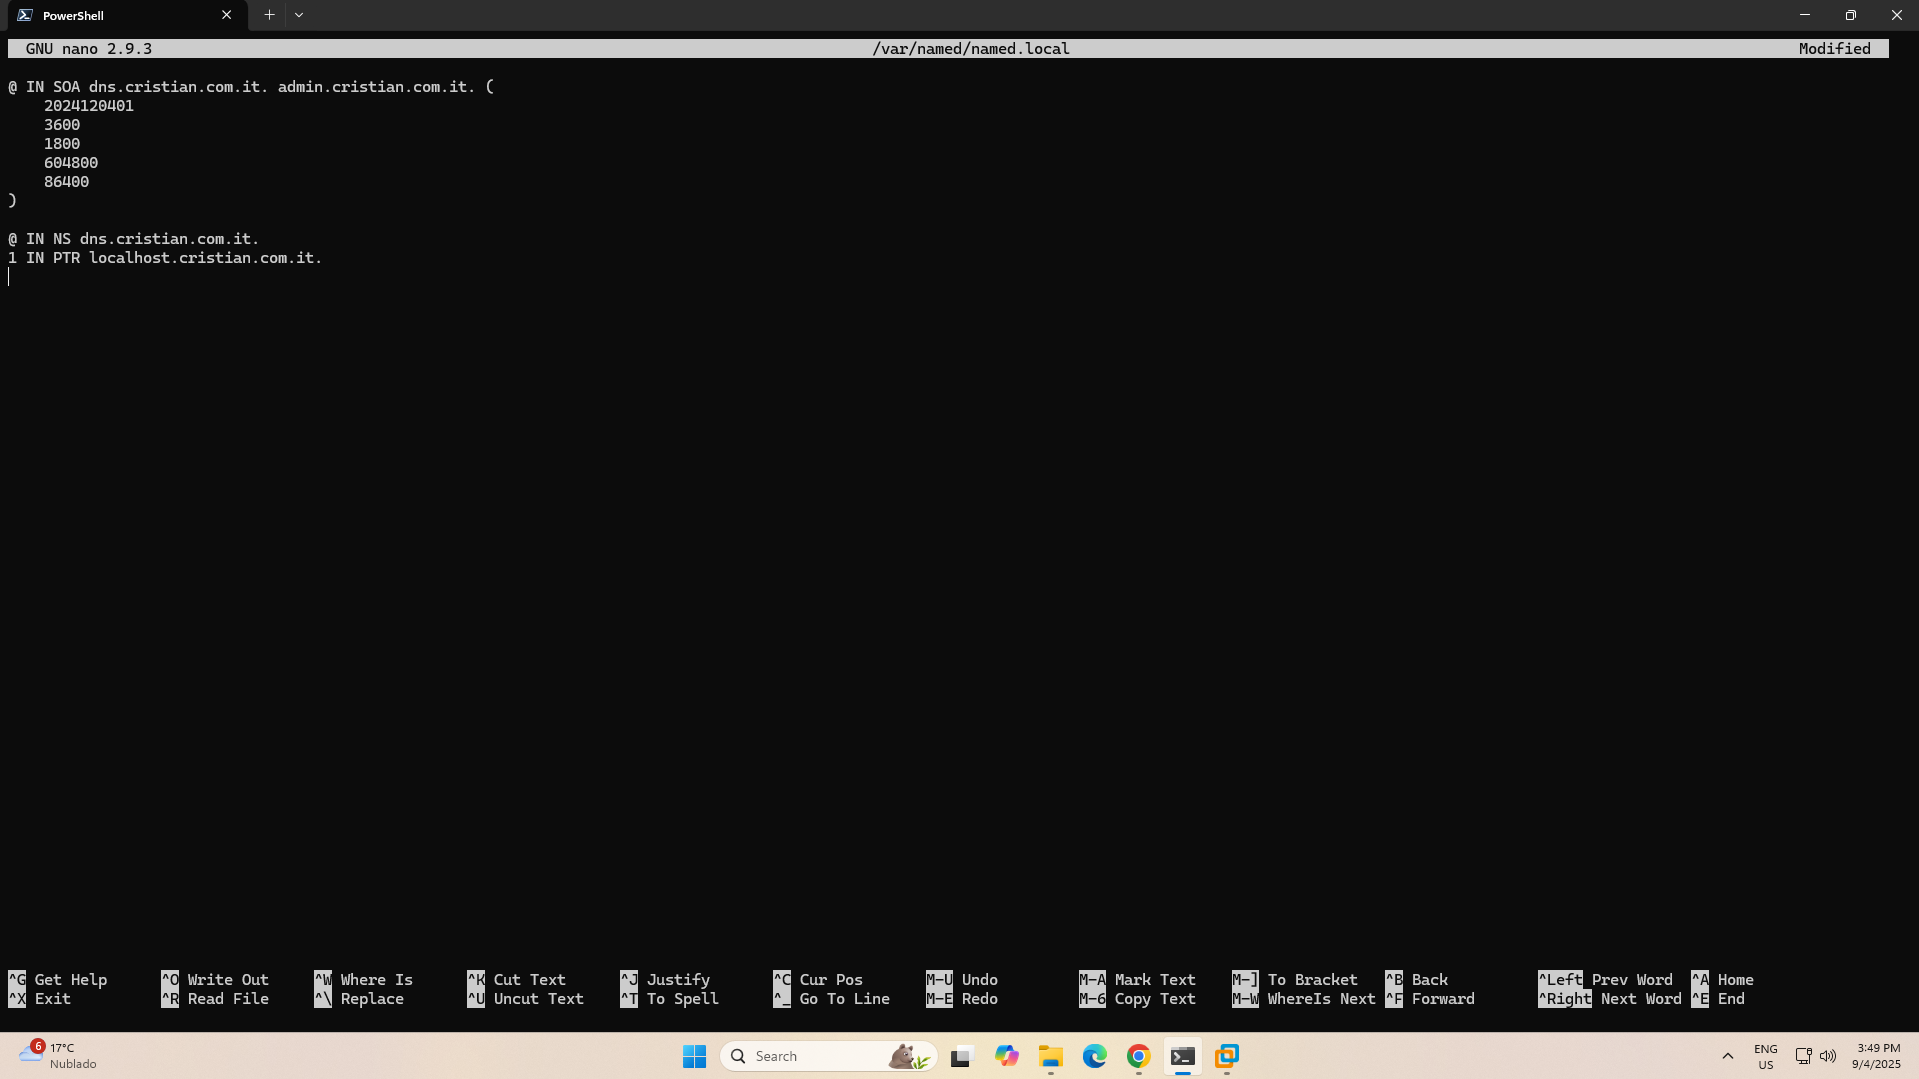
\includegraphics[keepaspectratio,alt={image.png}]{Third - DNS 263f56fc503e80ddb361c216e75fd3bf/image 14.png}}
\caption{image.png}
\end{figure}

\subsection{Paso 7: Iniciar el
servicio}\label{paso-7-iniciar-el-servicio}

\begin{Shaded}
\begin{Highlighting}[]
\ExtensionTok{solaris\#}\NormalTok{ /usr/sbin/named}
\end{Highlighting}
\end{Shaded}

\subsection{Paso 8: Verificar
funcionamiento}\label{paso-8-verificar-funcionamiento}

\begin{Shaded}
\begin{Highlighting}[]
    \ExtensionTok{solaris\#}\NormalTok{ ps }\AttributeTok{{-}ef} \KeywordTok{|} \FunctionTok{grep}\NormalTok{ named}
    \ExtensionTok{solaris\#}\NormalTok{ netstat }\AttributeTok{{-}an} \KeywordTok{|} \FunctionTok{grep}\NormalTok{ :53}
\end{Highlighting}
\end{Shaded}

\begin{center}\rule{0.5\linewidth}{0.5pt}\end{center}

\section{SOLARIS - PRIMARY DNS SERVER CONFIGURATION - SOLARIS AS SECOND
DNS SERVER FOR SLACKWARE
✅}\label{solaris---primary-dns-server-configuration---solaris-as-second-dns-server-for-slackware}

\subsection{Server Information}\label{server-information}

\begin{itemize}
\tightlist
\item
  \textbf{Solaris IP}: 10.2.77.178
\item
  \textbf{Primary Domain}: cristian.com.it
\item
  \textbf{Secondary Domain}: andersson.org.uk (from Slackware)
\end{itemize}

\subsection{Step 1: Check if BIND is
Installed}\label{step-1-check-if-bind-is-installed}

\begin{Shaded}
\begin{Highlighting}[]
\ExtensionTok{solaris\#}\NormalTok{ which named}
\ExtensionTok{solaris\#}\NormalTok{ ls /usr/sbin/named}
\end{Highlighting}
\end{Shaded}

\begin{figure}
\centering
\pandocbounded{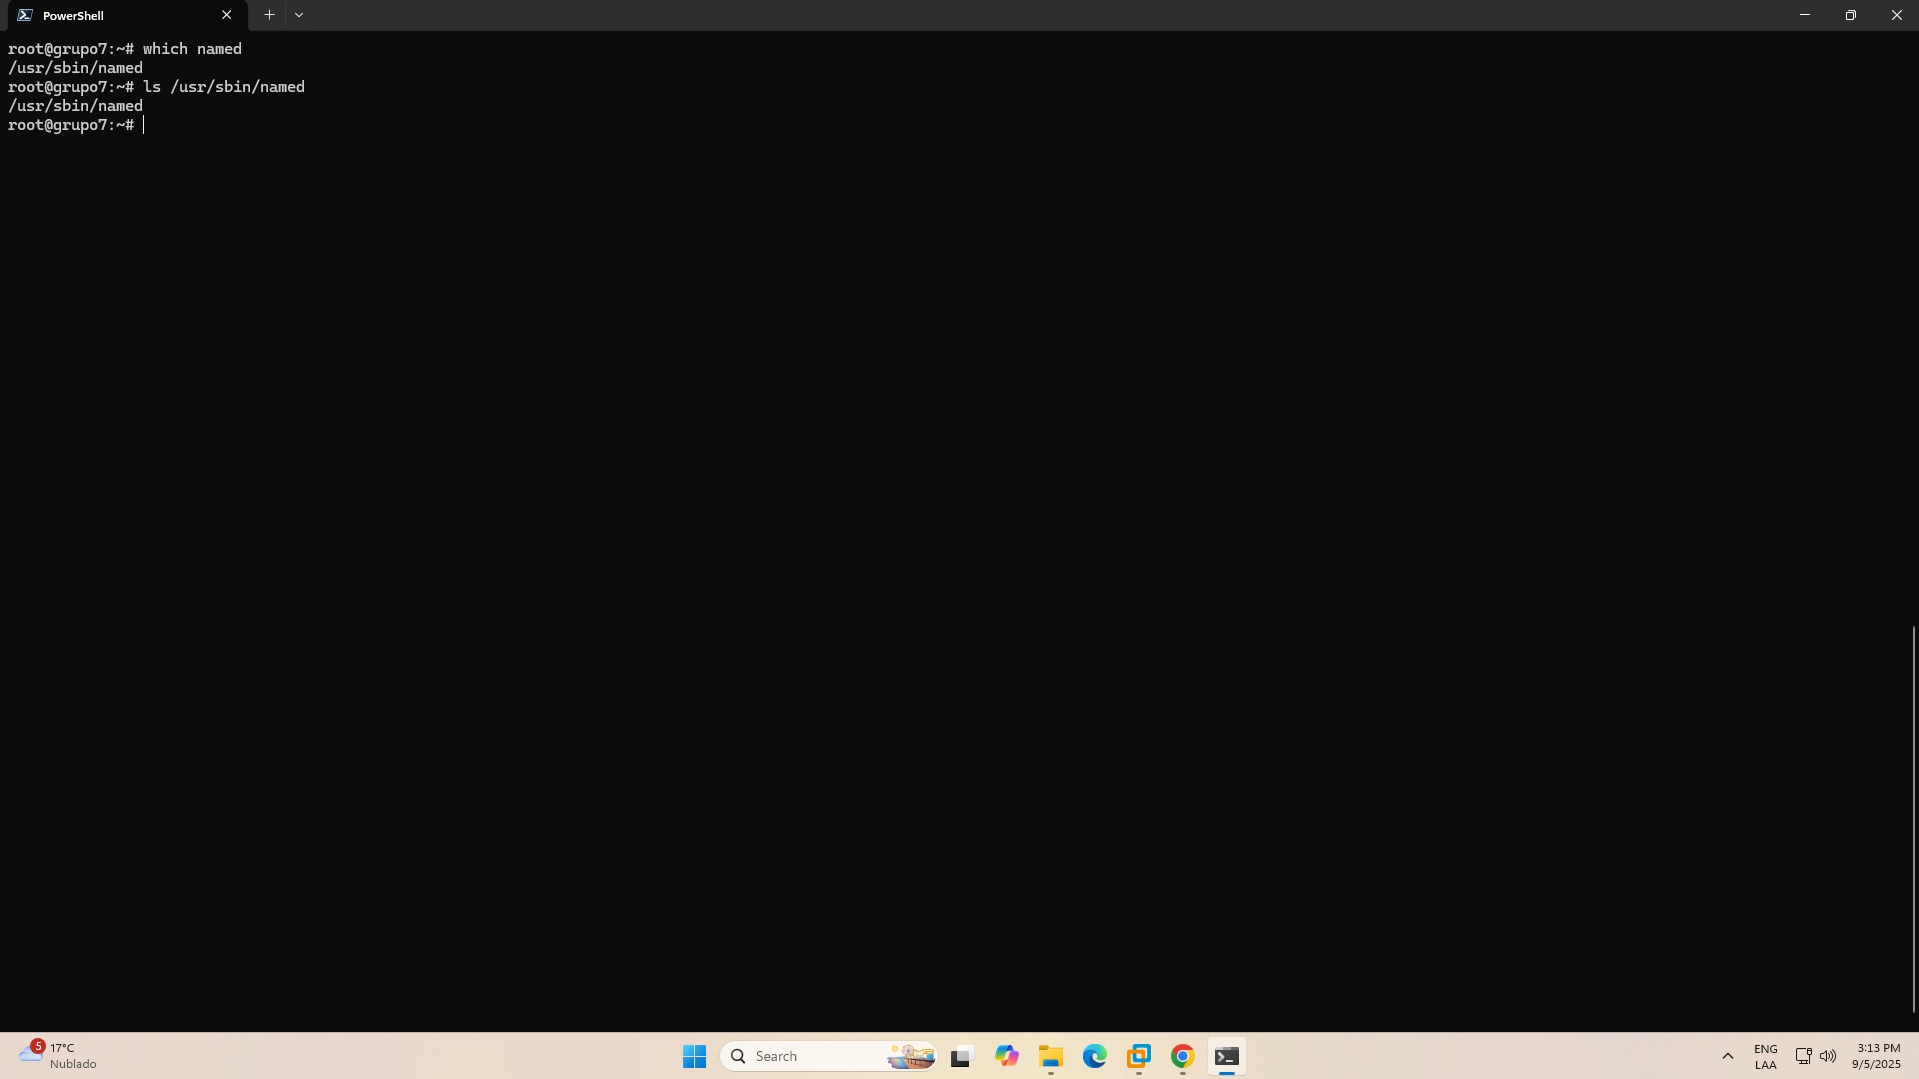
\includegraphics[keepaspectratio,alt={image.png}]{Third - DNS 263f56fc503e80ddb361c216e75fd3bf/image 15.png}}
\caption{image.png}
\end{figure}

\st{If BIND is not installed:}

\begin{Shaded}
\begin{Highlighting}[]
\CommentTok{\# Install BIND package}
\ExtensionTok{solaris\#}\NormalTok{ pkgadd }\AttributeTok{{-}d}\NormalTok{ /cdrom/sol\_}\PreprocessorTok{*}\NormalTok{/Product SUNWbind}
\CommentTok{\# or}
\ExtensionTok{solaris\#}\NormalTok{ pkg install bind}
\end{Highlighting}
\end{Shaded}

\subsection{Step 2: Create Directory
Structure}\label{step-2-create-directory-structure}

\begin{Shaded}
\begin{Highlighting}[]
\ExtensionTok{solaris\#}\NormalTok{ mkdir }\AttributeTok{{-}p}\NormalTok{ /var/named}
\ExtensionTok{solaris\#}\NormalTok{ cd /var/named}
\end{Highlighting}
\end{Shaded}

\begin{figure}
\centering
\pandocbounded{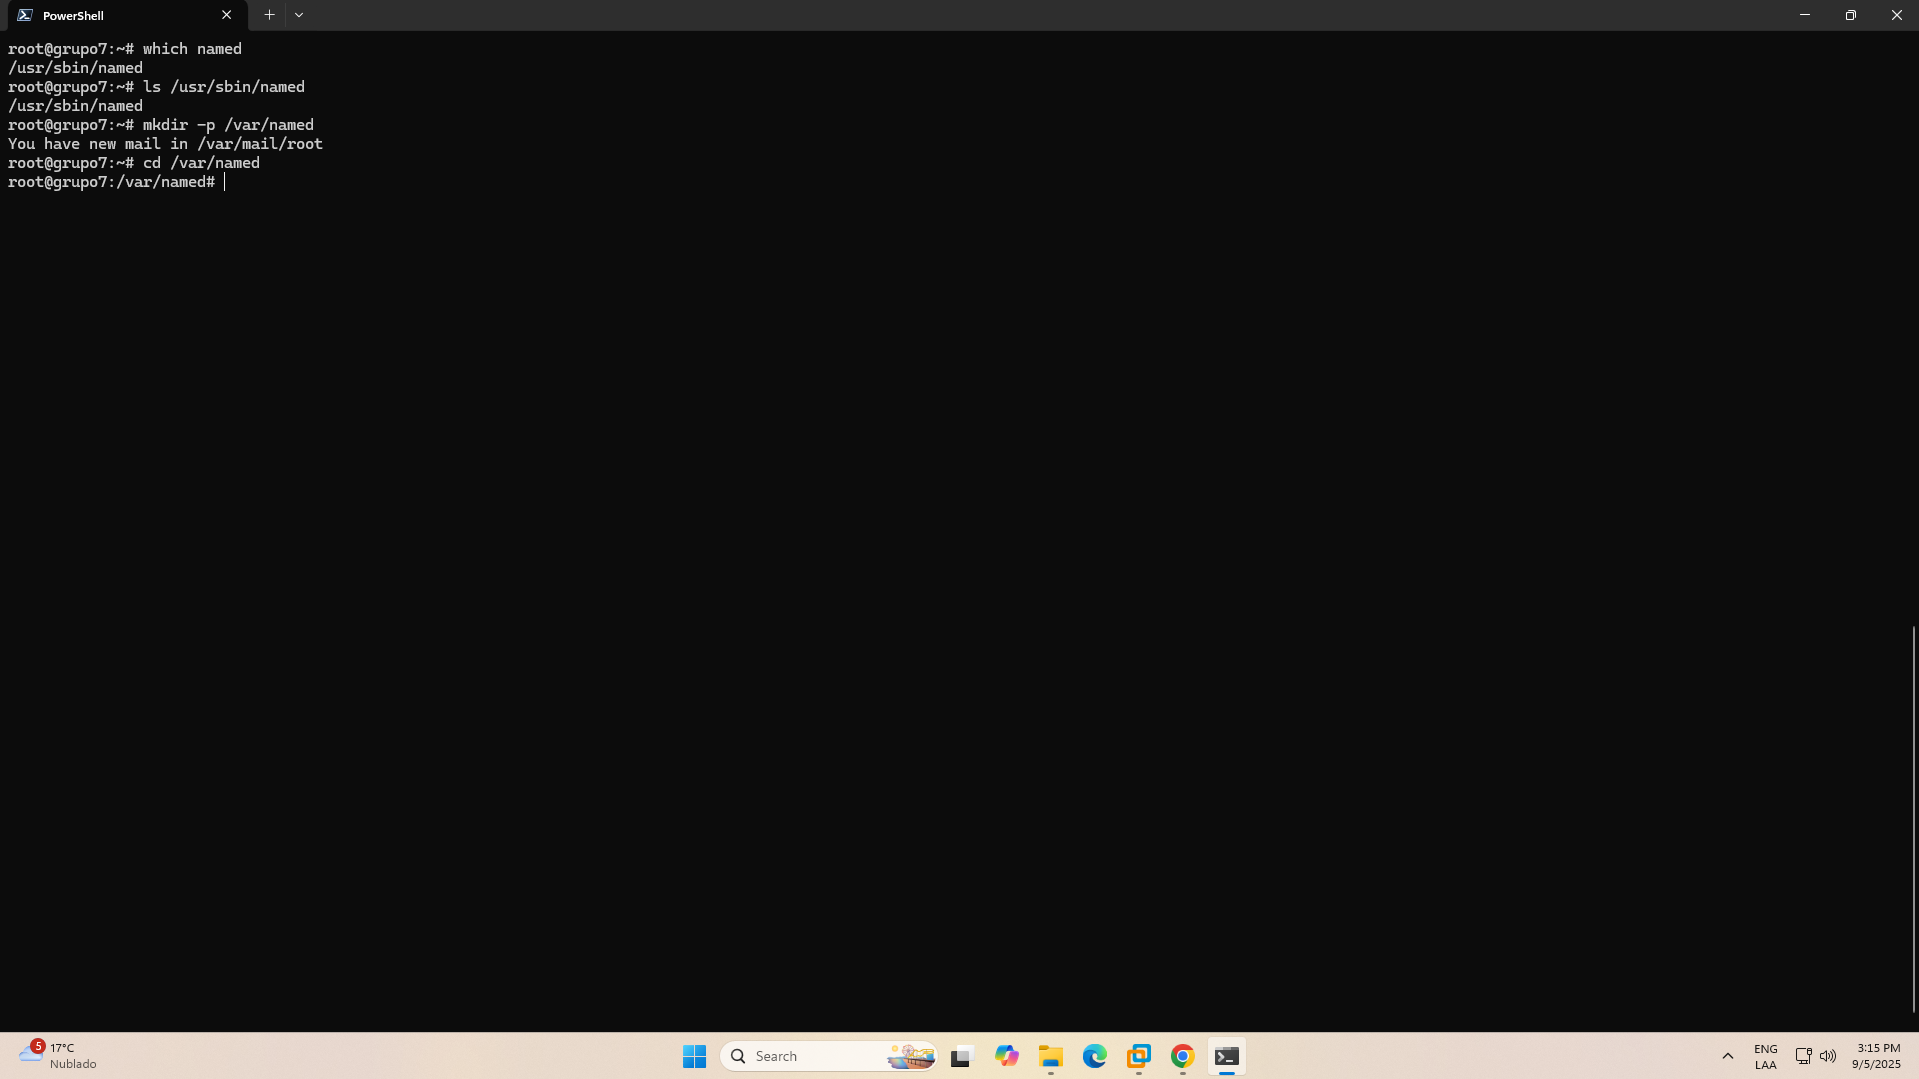
\includegraphics[keepaspectratio,alt={image.png}]{Third - DNS 263f56fc503e80ddb361c216e75fd3bf/image 16.png}}
\caption{image.png}
\end{figure}

\subsection{Step 3: Create Main Configuration
File}\label{step-3-create-main-configuration-file}

\begin{Shaded}
\begin{Highlighting}[]
\ExtensionTok{solaris\#}\NormalTok{ nano /etc/named.conf}
\end{Highlighting}
\end{Shaded}

\textbf{Content for /etc/named.conf:}

\begin{Shaded}
\begin{Highlighting}[]
\ExtensionTok{options}\NormalTok{ \{}
    \ExtensionTok{directory} \StringTok{"/var/named"}\KeywordTok{;}
    \ExtensionTok{allow{-}query}\NormalTok{ \{ any}\KeywordTok{;} \ErrorTok{\}}\KeywordTok{;}
    \ExtensionTok{recursion}\NormalTok{ yes}\KeywordTok{;}
    \ExtensionTok{listen{-}on}\NormalTok{ \{ any}\KeywordTok{;} \ErrorTok{\}}\KeywordTok{;}
    \ExtensionTok{listen{-}on{-}v6}\NormalTok{ \{ none}\KeywordTok{;} \ErrorTok{\}}\KeywordTok{;}
\ErrorTok{\}}\KeywordTok{;}

\ExtensionTok{//}\NormalTok{ Root zone}
\ExtensionTok{zone} \StringTok{"."}\NormalTok{ IN \{}
    \BuiltInTok{type}\NormalTok{ hint}\KeywordTok{;}
    \FunctionTok{file} \StringTok{"named.ca"}\KeywordTok{;}
\ErrorTok{\}}\KeywordTok{;}

\ExtensionTok{//}\NormalTok{ PRIMARY zone for cristian.com.it}
\ExtensionTok{zone} \StringTok{"cristian.com.it"}\NormalTok{ IN \{}
    \BuiltInTok{type}\NormalTok{ master}\KeywordTok{;}
    \FunctionTok{file} \StringTok{"cristian.com.it.zone"}\KeywordTok{;}
    \ExtensionTok{allow{-}transfer}\NormalTok{ \{ 10.2.77.176}\KeywordTok{;} \ErrorTok{\}}\KeywordTok{;}  \ExtensionTok{//}\NormalTok{ Allow Slackware to transfer}
\ErrorTok{\}}\KeywordTok{;}

\ExtensionTok{//}\NormalTok{ SECONDARY zone for andersson.org.uk }\ErrorTok{(}\ExtensionTok{from}\NormalTok{ Slackware}\KeywordTok{)}
\ExtensionTok{zone} \StringTok{"andersson.org.uk"}\NormalTok{ IN \{}
    \BuiltInTok{type}\NormalTok{ slave}\KeywordTok{;}
    \FunctionTok{file} \StringTok{"andersson.org.uk.slave"}\KeywordTok{;}
    \ExtensionTok{masters}\NormalTok{ \{ 10.2.77.176}\KeywordTok{;} \ErrorTok{\}}\KeywordTok{;}
\ErrorTok{\}}\KeywordTok{;}

\ExtensionTok{//}\NormalTok{ Localhost zones}
\ExtensionTok{zone} \StringTok{"localhost"}\NormalTok{ IN \{}
    \BuiltInTok{type}\NormalTok{ master}\KeywordTok{;}
    \FunctionTok{file} \StringTok{"localhost.zone"}\KeywordTok{;}
    \ExtensionTok{allow{-}update}\NormalTok{ \{ none}\KeywordTok{;} \ErrorTok{\}}\KeywordTok{;}
\ErrorTok{\}}\KeywordTok{;}

\ExtensionTok{zone} \StringTok{"0.0.127.in{-}addr.arpa"}\NormalTok{ IN \{}
    \BuiltInTok{type}\NormalTok{ master}\KeywordTok{;}
    \FunctionTok{file} \StringTok{"named.local"}\KeywordTok{;}
    \ExtensionTok{allow{-}update}\NormalTok{ \{ none}\KeywordTok{;} \ErrorTok{\}}\KeywordTok{;}
\ErrorTok{\}}\KeywordTok{;}
\end{Highlighting}
\end{Shaded}

\begin{figure}
\centering
\pandocbounded{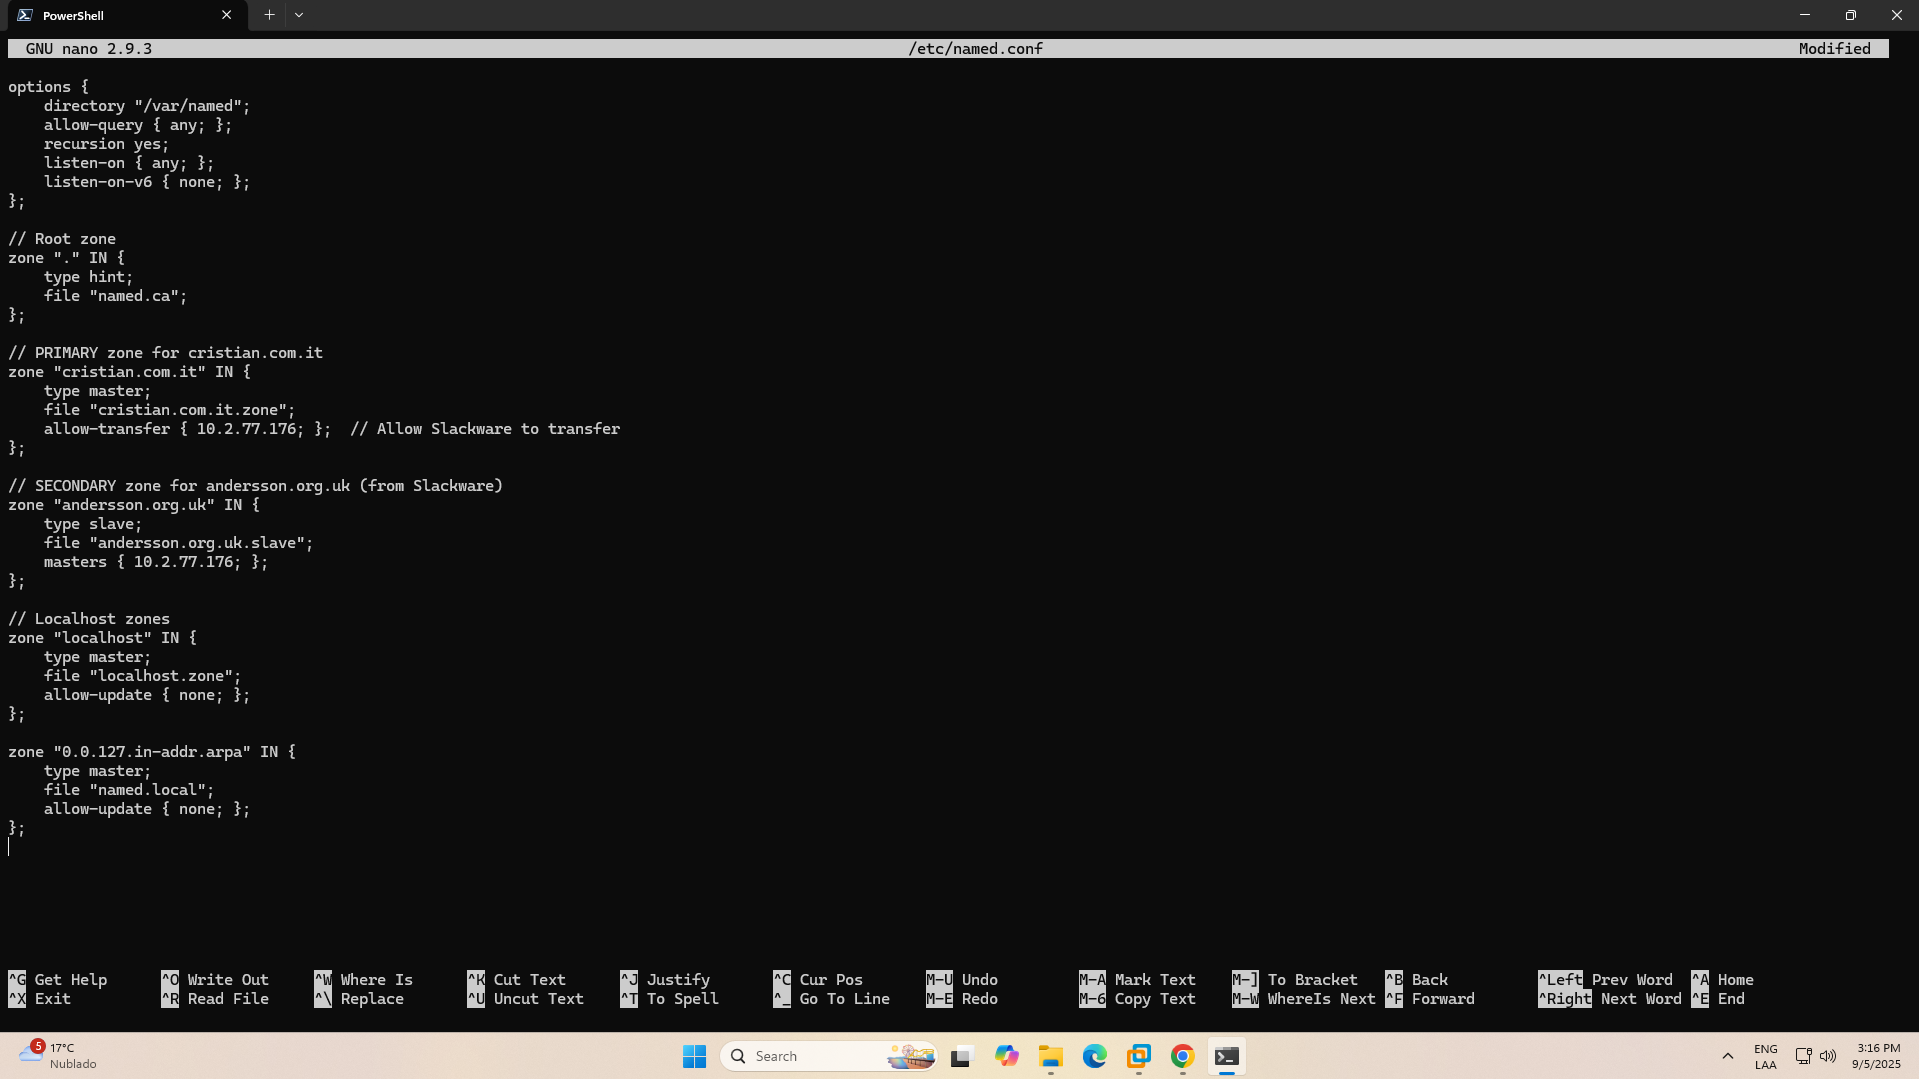
\includegraphics[keepaspectratio,alt={image.png}]{Third - DNS 263f56fc503e80ddb361c216e75fd3bf/image 17.png}}
\caption{image.png}
\end{figure}

\subsection{Step 4: Create Root Servers
File}\label{step-4-create-root-servers-file}

\begin{Shaded}
\begin{Highlighting}[]
\ExtensionTok{solaris\#}\NormalTok{ nano /var/named/named.ca}
\end{Highlighting}
\end{Shaded}

\textbf{Content for named.ca:}

\begin{Shaded}
\begin{Highlighting}[]
\KeywordTok{;}
\KeywordTok{;} \ExtensionTok{Root}\NormalTok{ name servers }\ErrorTok{(}\ExtensionTok{simplified}\KeywordTok{)}
\KeywordTok{;}
\BuiltInTok{.}\NormalTok{                        3600000      NS    A.ROOT{-}SERVERS.NET.}
\BuiltInTok{.}\NormalTok{                        3600000      NS    B.ROOT{-}SERVERS.NET.}
\BuiltInTok{.}\NormalTok{                        3600000      NS    C.ROOT{-}SERVERS.NET.}

\ExtensionTok{A.ROOT{-}SERVERS.NET.}\NormalTok{      3600000      A     198.41.0.4}
\ExtensionTok{B.ROOT{-}SERVERS.NET.}\NormalTok{      3600000      A     199.9.14.201}
\ExtensionTok{C.ROOT{-}SERVERS.NET.}\NormalTok{      3600000      A     192.33.4.12}
\end{Highlighting}
\end{Shaded}

\begin{figure}
\centering
\pandocbounded{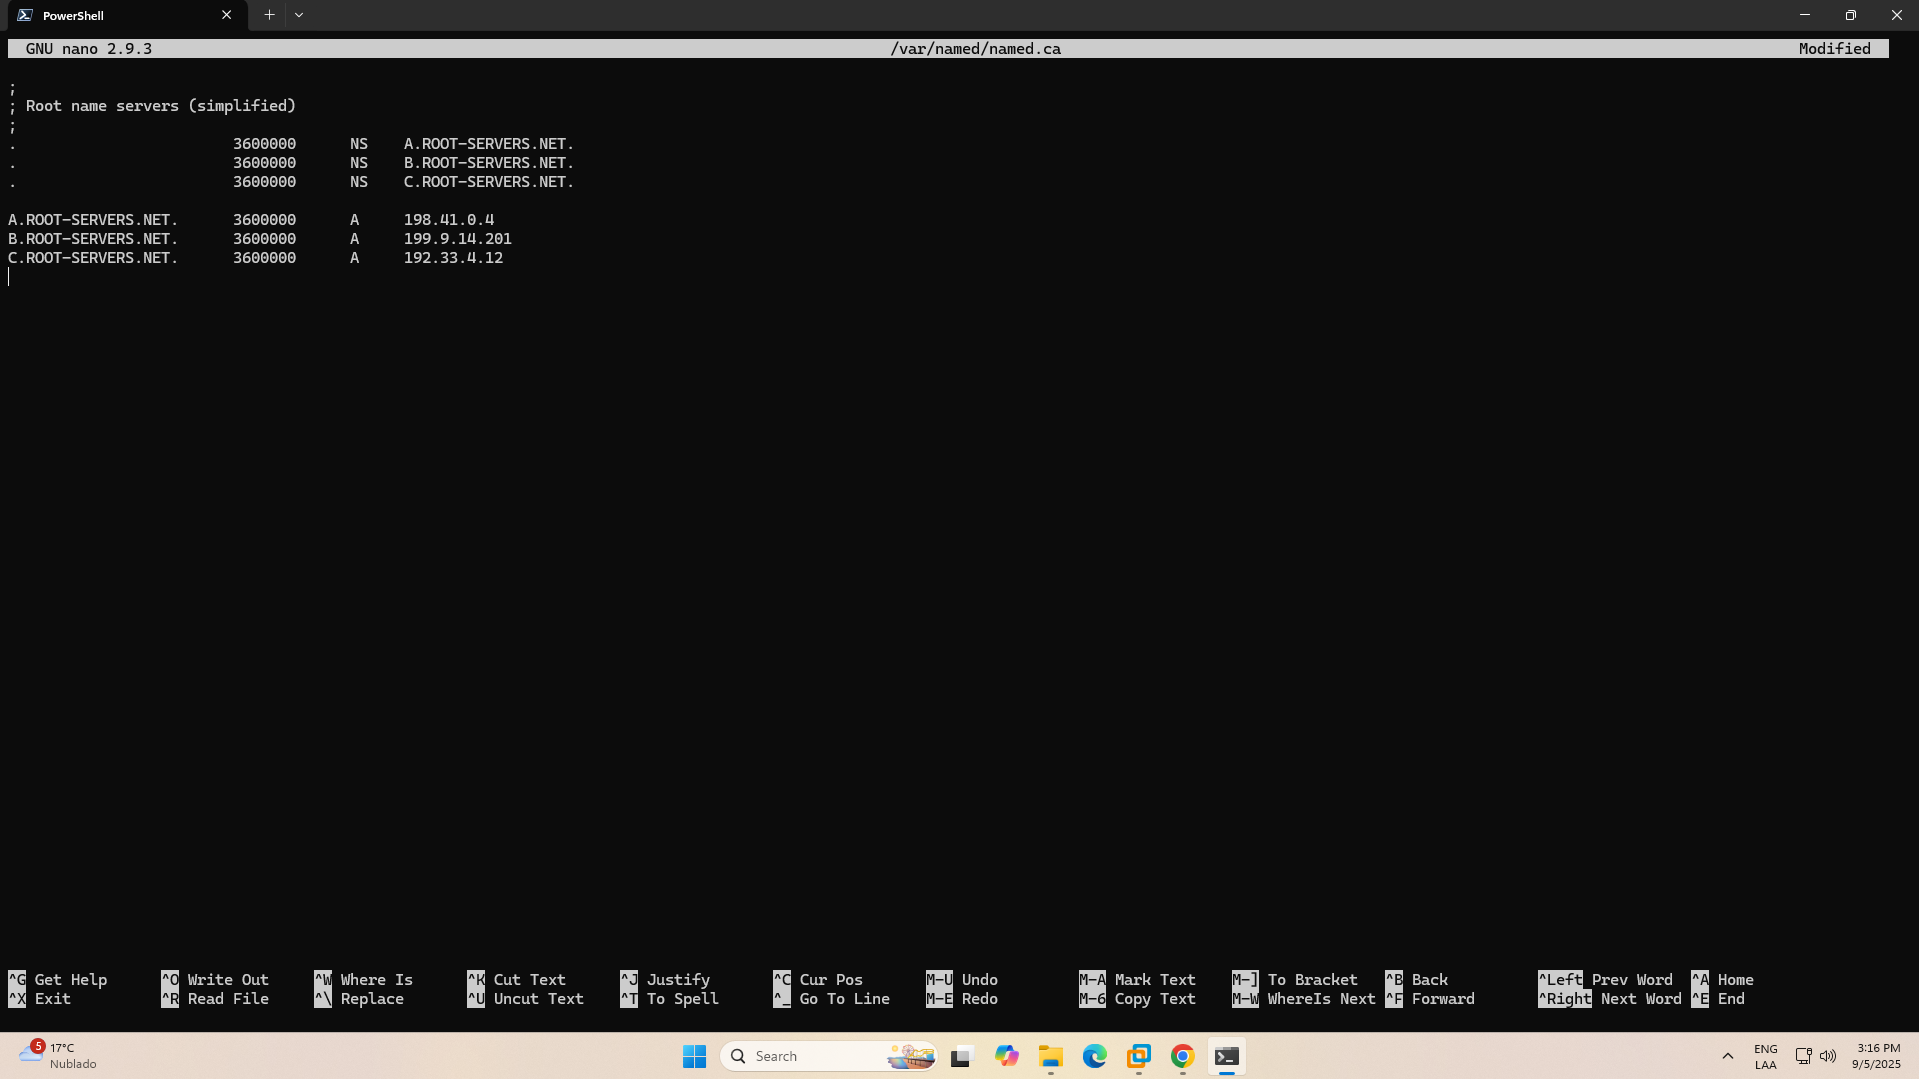
\includegraphics[keepaspectratio,alt={image.png}]{Third - DNS 263f56fc503e80ddb361c216e75fd3bf/image 18.png}}
\caption{image.png}
\end{figure}

\subsection{Step 5: Create Zone File for
cristian.com.it}\label{step-5-create-zone-file-for-cristian.com.it}

\begin{Shaded}
\begin{Highlighting}[]
\ExtensionTok{solaris\#}\NormalTok{ nano /var/named/cristian.com.it.zone}
\end{Highlighting}
\end{Shaded}

\textbf{Content for cristian.com.it.zone:}

\begin{Shaded}
\begin{Highlighting}[]
\KeywordTok{;}
\KeywordTok{;} \ExtensionTok{Zone}\NormalTok{ file for cristian.com.it}
\KeywordTok{;}
\VariableTok{$TTL}\NormalTok{ 86400}
\ExtensionTok{@}\NormalTok{       IN      SOA     dns.cristian.com.it. admin.cristian.com.it. }\ErrorTok{(}
                        \ExtensionTok{2024120401}      \KeywordTok{;} \ExtensionTok{Serial} \ErrorTok{(}\ExtensionTok{YYYYMMDDXX}\KeywordTok{)}
                        \ExtensionTok{3600}            \KeywordTok{;} \ExtensionTok{Refresh} \ErrorTok{(}\ExtensionTok{1}\NormalTok{ hour}\KeywordTok{)}
                        \ExtensionTok{1800}            \KeywordTok{;} \ExtensionTok{Retry} \ErrorTok{(}\ExtensionTok{30}\NormalTok{ minutes}\KeywordTok{)}
                        \ExtensionTok{604800}          \KeywordTok{;} \ExtensionTok{Expire} \ErrorTok{(}\ExtensionTok{1}\NormalTok{ week}\KeywordTok{)}
                        \ExtensionTok{86400}           \KeywordTok{;} \ExtensionTok{Minimum}\NormalTok{ TTL }\ErrorTok{(}\ExtensionTok{1}\NormalTok{ day}\KeywordTok{)}
\KeywordTok{)}

\KeywordTok{;} \ExtensionTok{Name}\NormalTok{ Server}
\ExtensionTok{@}\NormalTok{               IN      NS      dns.cristian.com.it.}

\KeywordTok{;} \ExtensionTok{IPv4}\NormalTok{ addresses }\ErrorTok{(}\ExtensionTok{A}\NormalTok{ records}\KeywordTok{)}
\ExtensionTok{dns}\NormalTok{             IN      A       10.2.77.178}
\ExtensionTok{server1}\NormalTok{         IN      A       10.2.77.180}
\ExtensionTok{server2}\NormalTok{         IN      A       10.2.77.181}
\ExtensionTok{server3}\NormalTok{         IN      A       10.2.77.182}

\KeywordTok{;} \ExtensionTok{IPv6}\NormalTok{ addresses }\ErrorTok{(}\ExtensionTok{AAAA}\NormalTok{ records}\KeywordTok{)}
\ExtensionTok{server1}\NormalTok{         IN      AAAA    2001:db8:1::1}
\ExtensionTok{server2}\NormalTok{         IN      AAAA    2001:db8:1::2}

\KeywordTok{;} \ExtensionTok{Aliases} \ErrorTok{(}\ExtensionTok{CNAME}\NormalTok{ records}\KeywordTok{)}
\ExtensionTok{www}\NormalTok{             IN      CNAME   server1.cristian.com.it.}
\ExtensionTok{mail}\NormalTok{            IN      CNAME   server2.cristian.com.it.}
\ExtensionTok{web}\NormalTok{             IN      CNAME   server1.cristian.com.it.}
\FunctionTok{ftp}\NormalTok{             IN      CNAME   server3.cristian.com.it.}
\end{Highlighting}
\end{Shaded}

\begin{figure}
\centering
\pandocbounded{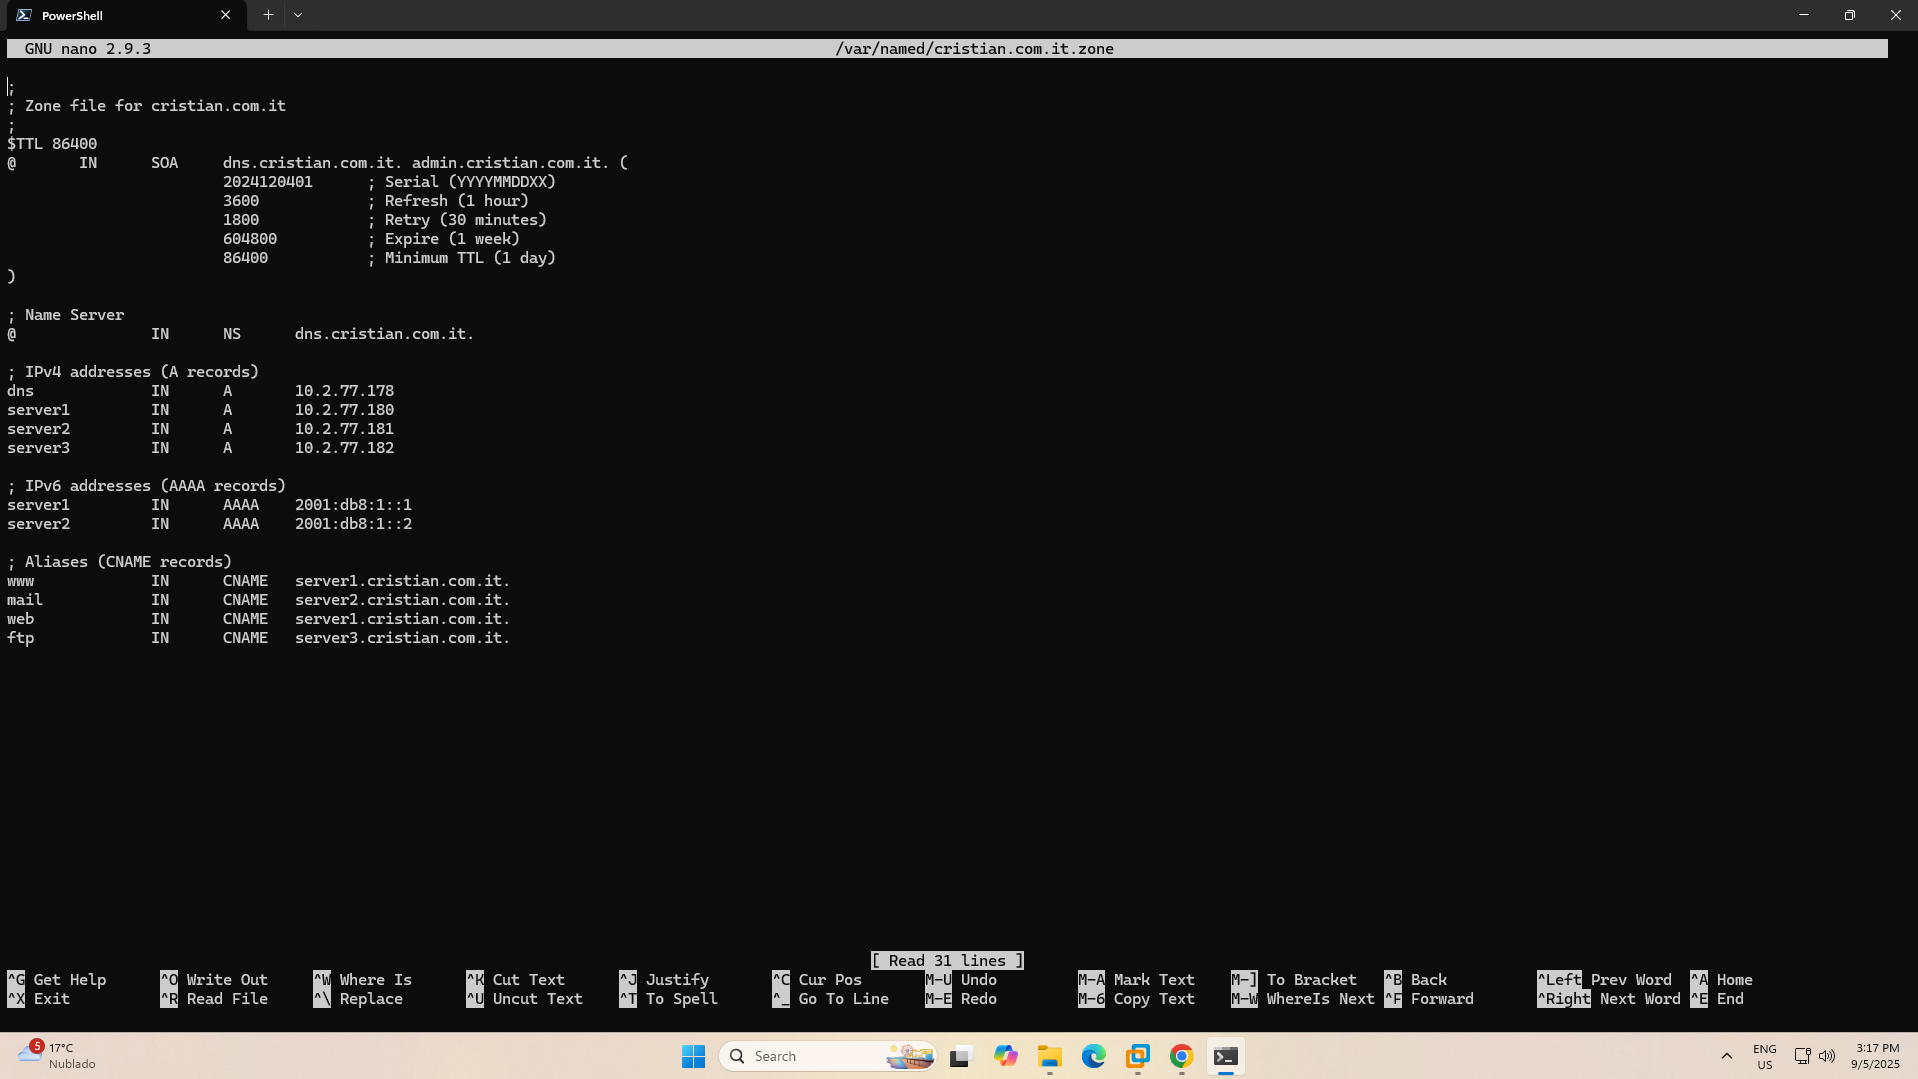
\includegraphics[keepaspectratio,alt={image.png}]{Third - DNS 263f56fc503e80ddb361c216e75fd3bf/image 19.png}}
\caption{image.png}
\end{figure}

\subsection{Step 6: Create Localhost Zone
Files}\label{step-6-create-localhost-zone-files}

\begin{Shaded}
\begin{Highlighting}[]
\ExtensionTok{solaris\#}\NormalTok{ nano /var/named/localhost.zone}
\end{Highlighting}
\end{Shaded}

\textbf{Content for localhost.zone:}

\begin{Shaded}
\begin{Highlighting}[]
\VariableTok{$TTL}\NormalTok{ 86400}
\ExtensionTok{@}\NormalTok{       IN      SOA     dns.cristian.com.it. admin.cristian.com.it. }\ErrorTok{(}
                        \ExtensionTok{2024120401}      \KeywordTok{;} \ExtensionTok{Serial}
                        \ExtensionTok{3600}            \KeywordTok{;} \ExtensionTok{Refresh}
                        \ExtensionTok{1800}            \KeywordTok{;} \ExtensionTok{Retry}
                        \ExtensionTok{604800}          \KeywordTok{;} \ExtensionTok{Expire}
                        \ExtensionTok{86400}           \KeywordTok{;} \ExtensionTok{Minimum}
\KeywordTok{)}

\ExtensionTok{@}\NormalTok{       IN      NS      dns.cristian.com.it.}
\ExtensionTok{@}\NormalTok{       IN      A       127.0.0.1}
\end{Highlighting}
\end{Shaded}

\begin{figure}
\centering
\pandocbounded{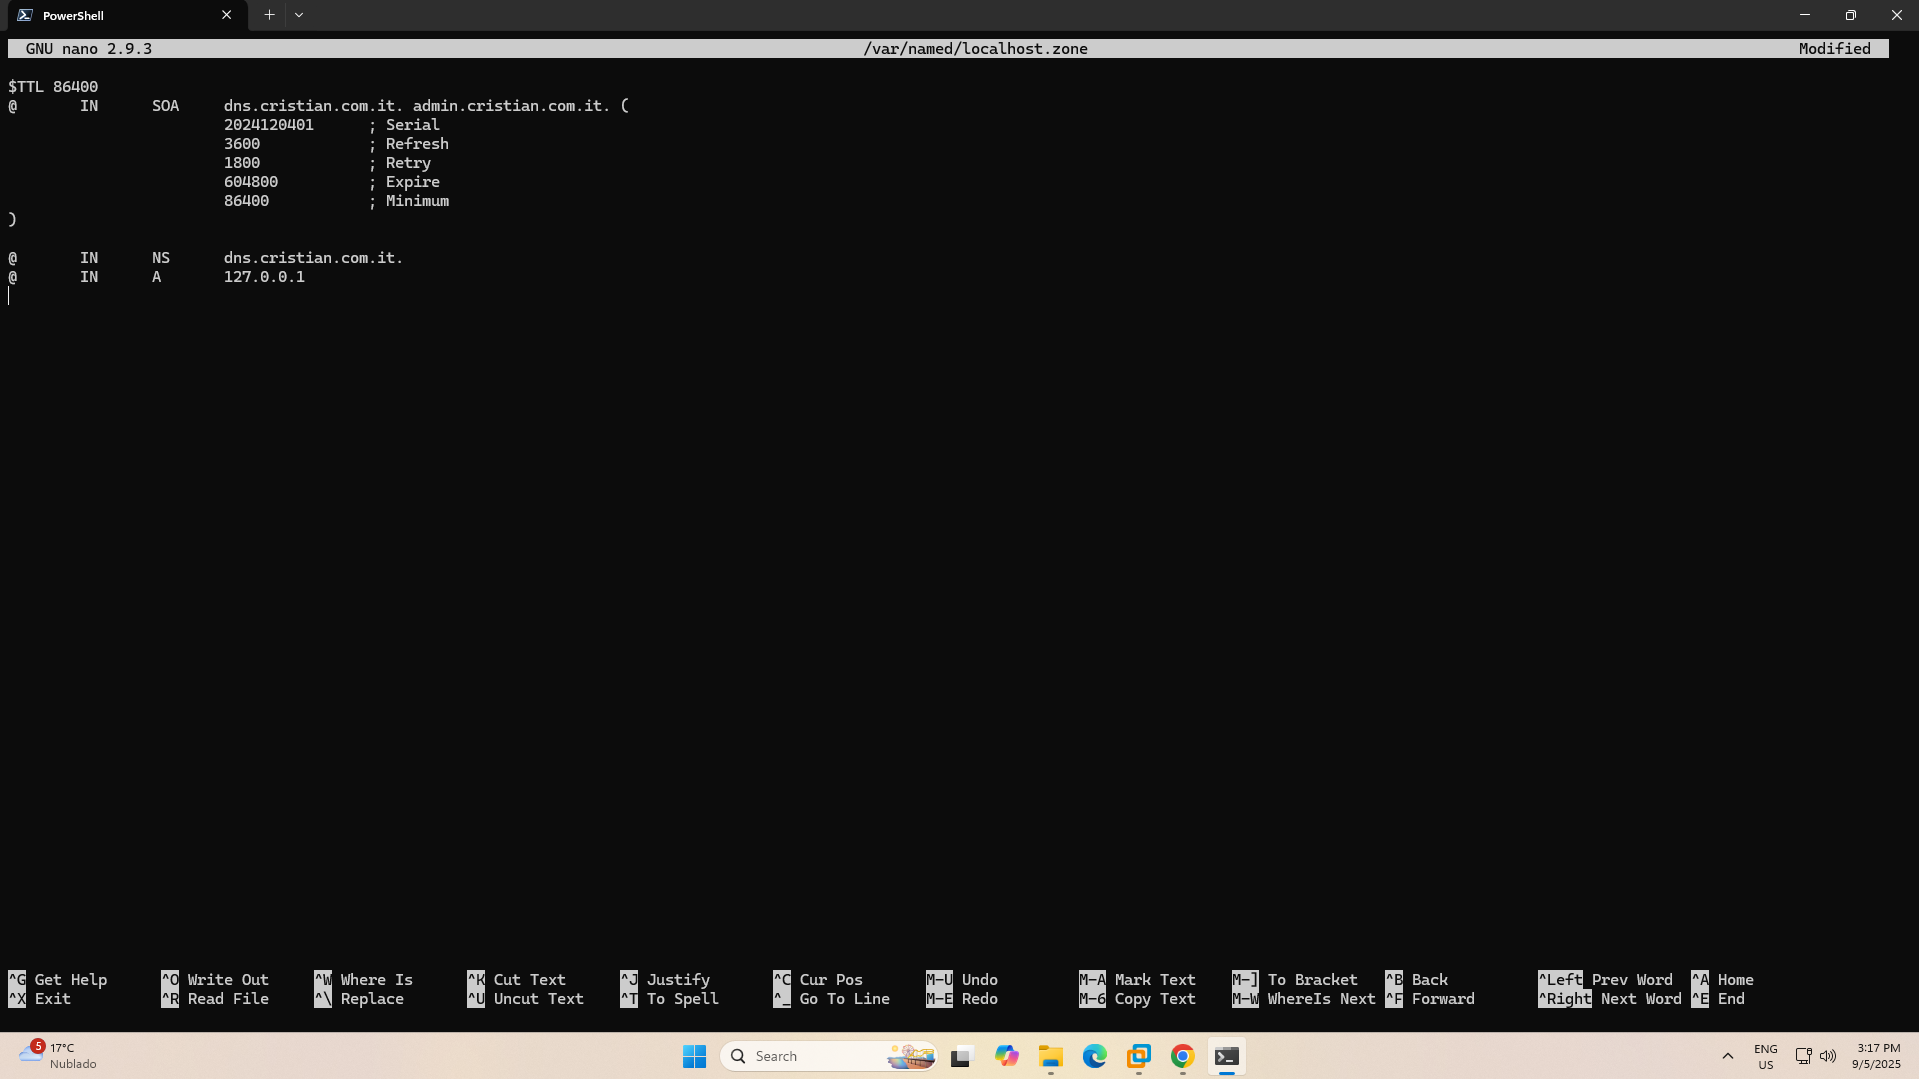
\includegraphics[keepaspectratio,alt={image.png}]{Third - DNS 263f56fc503e80ddb361c216e75fd3bf/image 20.png}}
\caption{image.png}
\end{figure}

\begin{Shaded}
\begin{Highlighting}[]
\ExtensionTok{solaris\#}\NormalTok{ nano /var/named/named.local}
\end{Highlighting}
\end{Shaded}

\textbf{Content for named.local:}

\begin{Shaded}
\begin{Highlighting}[]
\VariableTok{$TTL}\NormalTok{ 86400}
\ExtensionTok{@}\NormalTok{       IN      SOA     dns.cristian.com.it. admin.cristian.com.it. }\ErrorTok{(}
                        \ExtensionTok{2024120401}      \KeywordTok{;} \ExtensionTok{Serial}
                        \ExtensionTok{3600}            \KeywordTok{;} \ExtensionTok{Refresh}
                        \ExtensionTok{1800}            \KeywordTok{;} \ExtensionTok{Retry}
                        \ExtensionTok{604800}          \KeywordTok{;} \ExtensionTok{Expire}
                        \ExtensionTok{86400}           \KeywordTok{;} \ExtensionTok{Minimum}
\KeywordTok{)}

\ExtensionTok{@}\NormalTok{       IN      NS      dns.cristian.com.it.}
\ExtensionTok{1}\NormalTok{       IN      PTR     localhost.}
\end{Highlighting}
\end{Shaded}

\begin{figure}
\centering
\pandocbounded{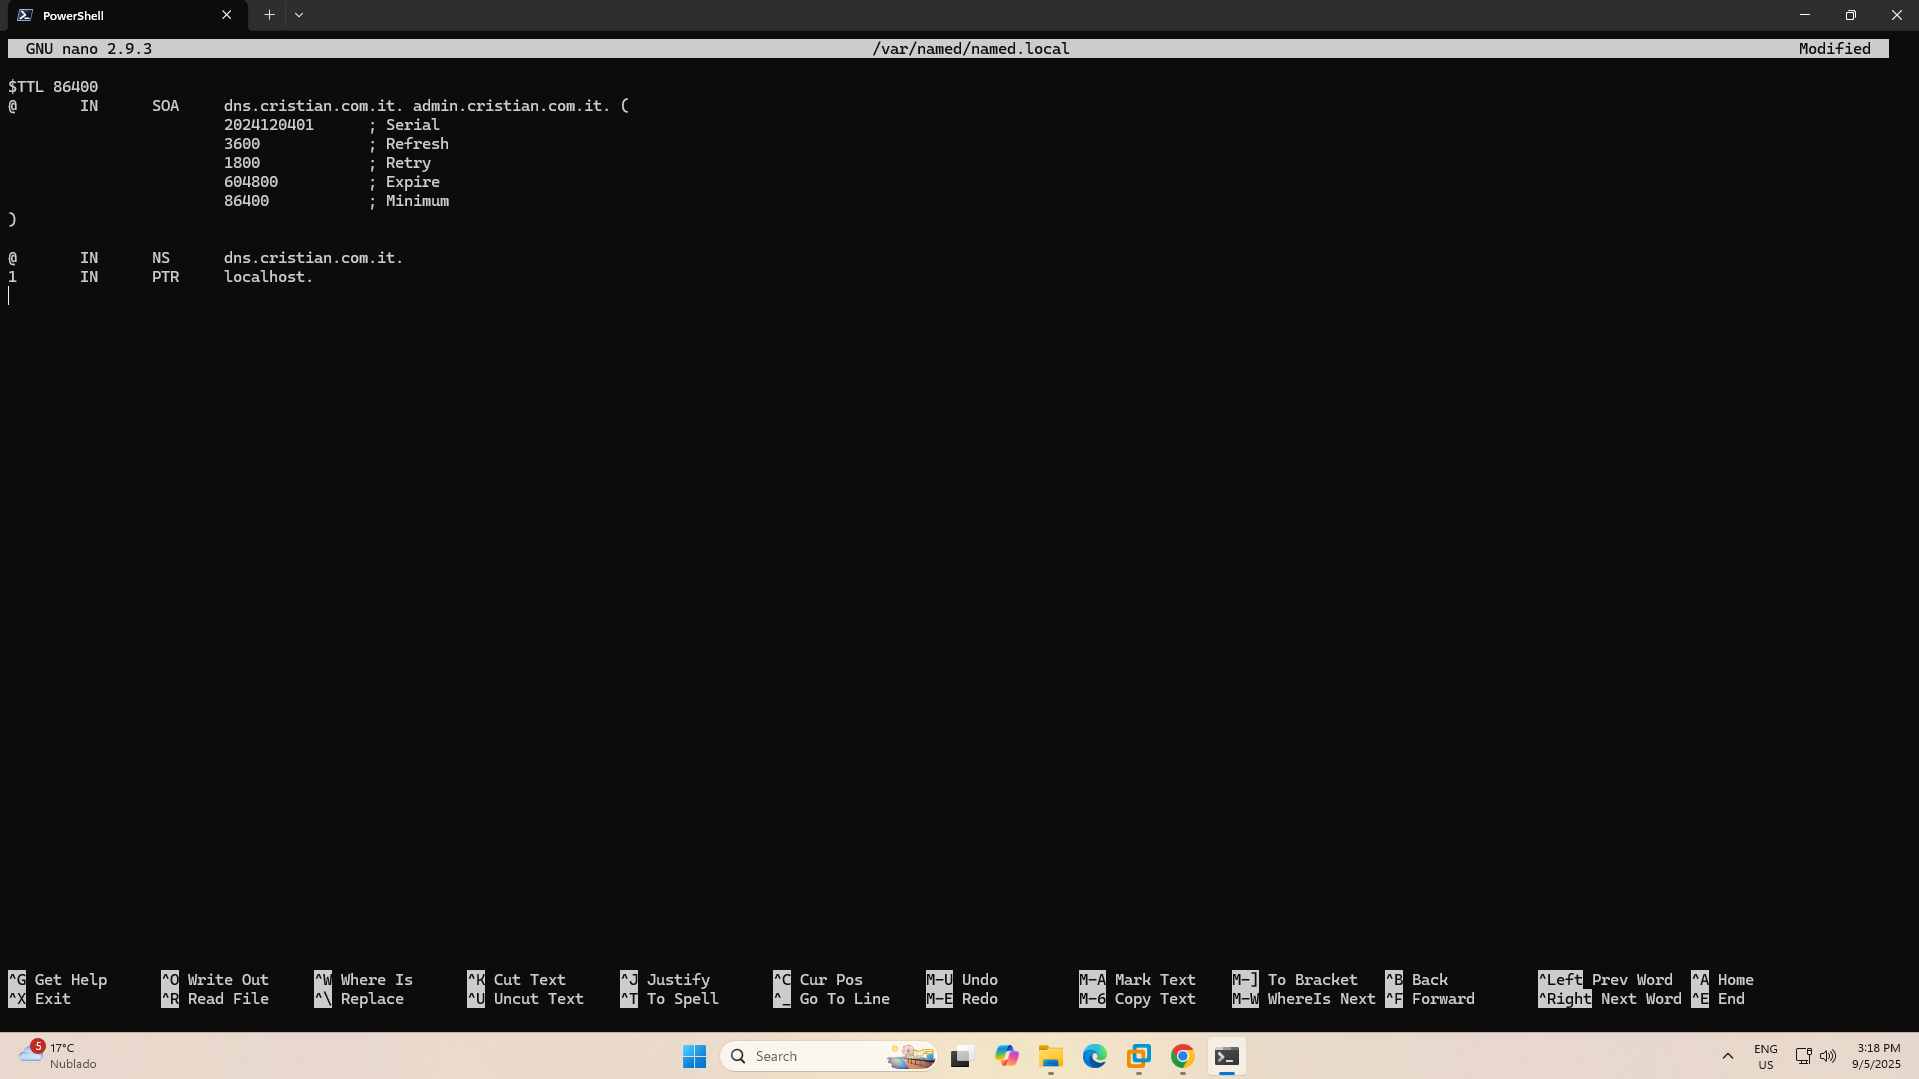
\includegraphics[keepaspectratio,alt={image.png}]{Third - DNS 263f56fc503e80ddb361c216e75fd3bf/image 21.png}}
\caption{image.png}
\end{figure}

\subsection{Step 7: Set Correct
Permissions}\label{step-7-set-correct-permissions}

\begin{Shaded}
\begin{Highlighting}[]
\FunctionTok{chown} \AttributeTok{{-}R}\NormalTok{ named:named /var/named}
\FunctionTok{chmod}\NormalTok{ 755 /var/named}
\FunctionTok{chmod}\NormalTok{ 644 /var/named/}\PreprocessorTok{*}
\FunctionTok{chown}\NormalTok{ named:named /etc/named.conf}
\FunctionTok{chmod}\NormalTok{ 644 /etc/named.conf}
\end{Highlighting}
\end{Shaded}

\begin{figure}
\centering
\pandocbounded{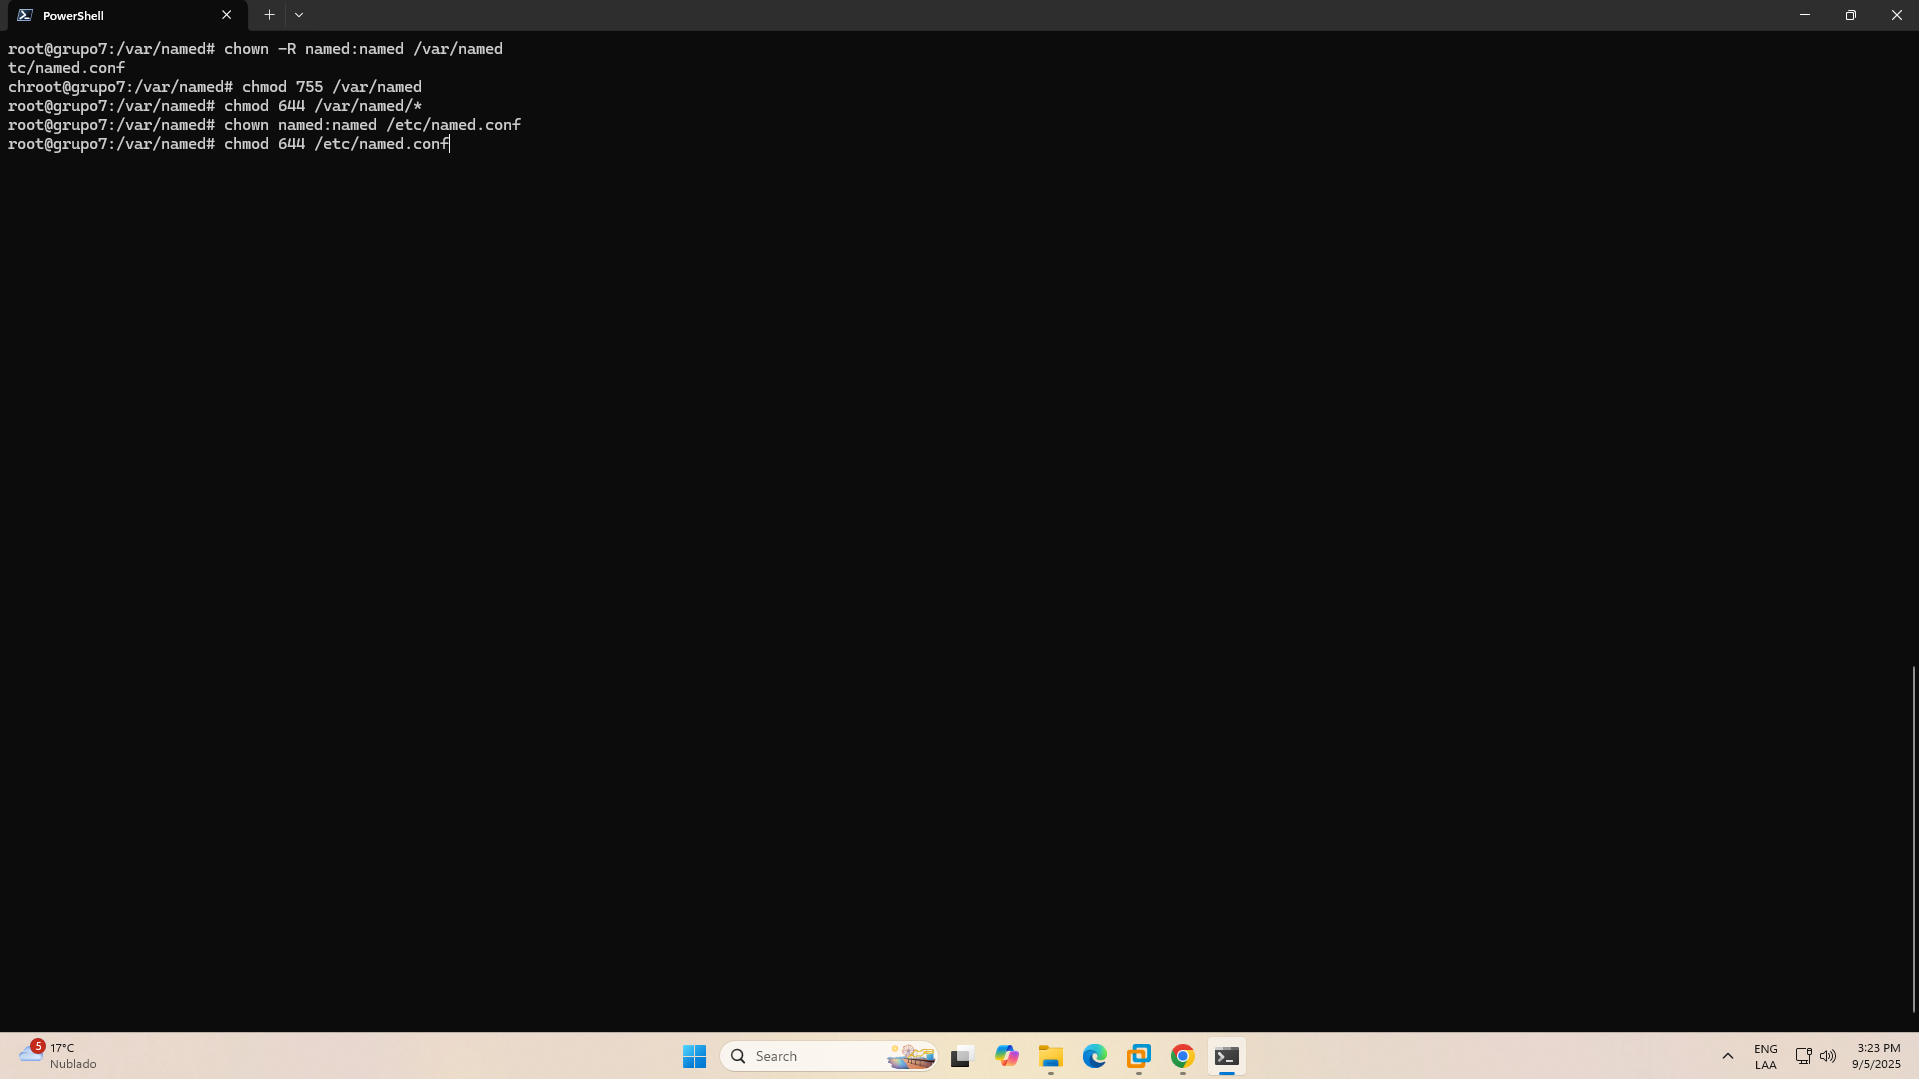
\includegraphics[keepaspectratio,alt={image.png}]{Third - DNS 263f56fc503e80ddb361c216e75fd3bf/image 22.png}}
\caption{image.png}
\end{figure}

\subsection{Step 8: Check Configuration
Syntax}\label{step-8-check-configuration-syntax}

\begin{Shaded}
\begin{Highlighting}[]
\CommentTok{\# Check main configuration}
\ExtensionTok{solaris\#}\NormalTok{ named{-}checkconf /etc/named.conf}

\CommentTok{\# Check zone file}
\ExtensionTok{solaris\#}\NormalTok{ named{-}checkzone cristian.com.it /var/named/cristian.com.it.zone}
\end{Highlighting}
\end{Shaded}

\textbf{Expected output:}

\begin{verbatim}
zone cristian.com.it/IN: loaded serial 2024120401
OK
\end{verbatim}

\begin{figure}
\centering
\pandocbounded{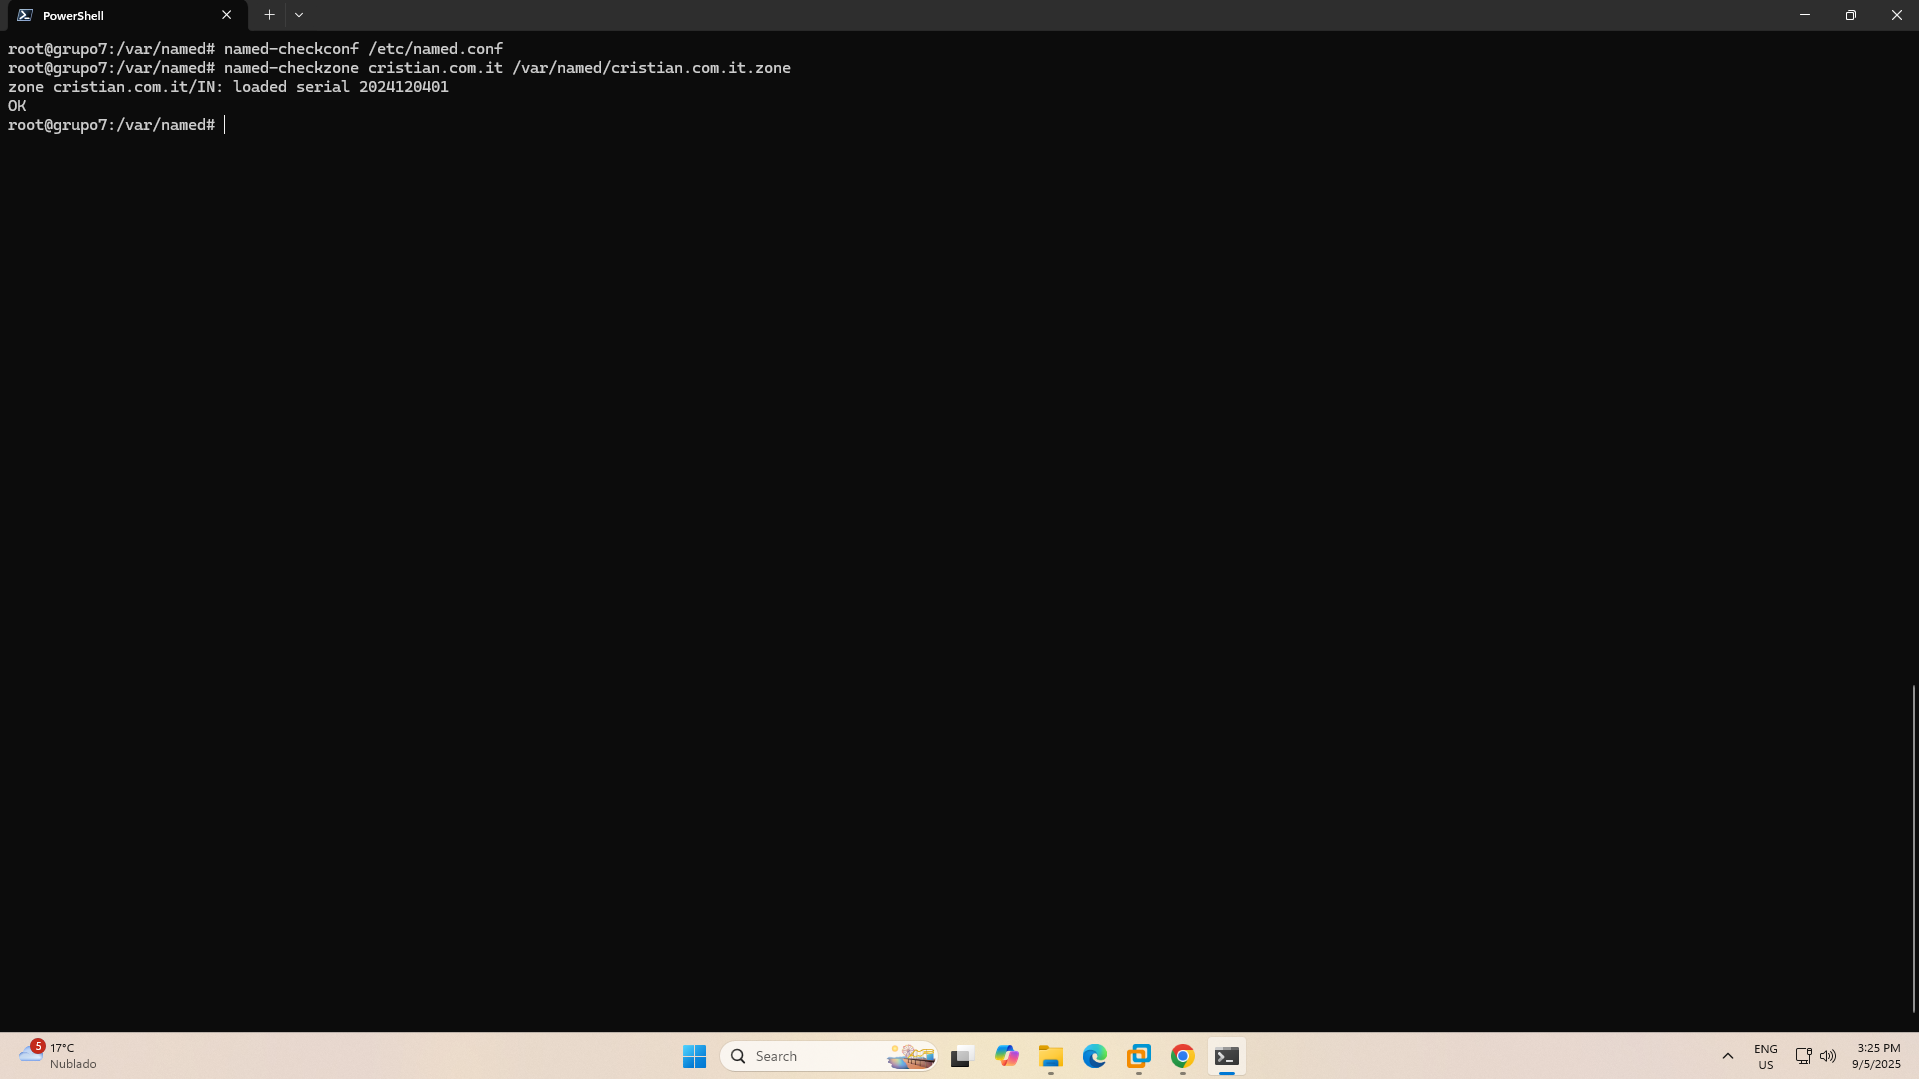
\includegraphics[keepaspectratio,alt={image.png}]{Third - DNS 263f56fc503e80ddb361c216e75fd3bf/image 23.png}}
\caption{image.png}
\end{figure}

\href{Third\%20-\%20DNS\%20263f56fc503e80ddb361c216e75fd3bf/Step8\%20didnt\%20work\%20265f56fc503e807a80cbcc525efe949d.md}{Step8
didnt work}

\subsection{Step 9: Start the DNS
Service}\label{step-9-start-the-dns-service}

\begin{Shaded}
\begin{Highlighting}[]
\CommentTok{\# Kill any existing named processes}
\ExtensionTok{solaris\#}\NormalTok{ pkill named}

\CommentTok{\# Start named service}
\ExtensionTok{solaris\#}\NormalTok{ /usr/sbin/named}

\CommentTok{\# Or start with logging (for debugging)}
\ExtensionTok{solaris\#}\NormalTok{ /usr/sbin/named }\AttributeTok{{-}f} \AttributeTok{{-}g} \KeywordTok{\&}
\end{Highlighting}
\end{Shaded}

\begin{figure}
\centering
\pandocbounded{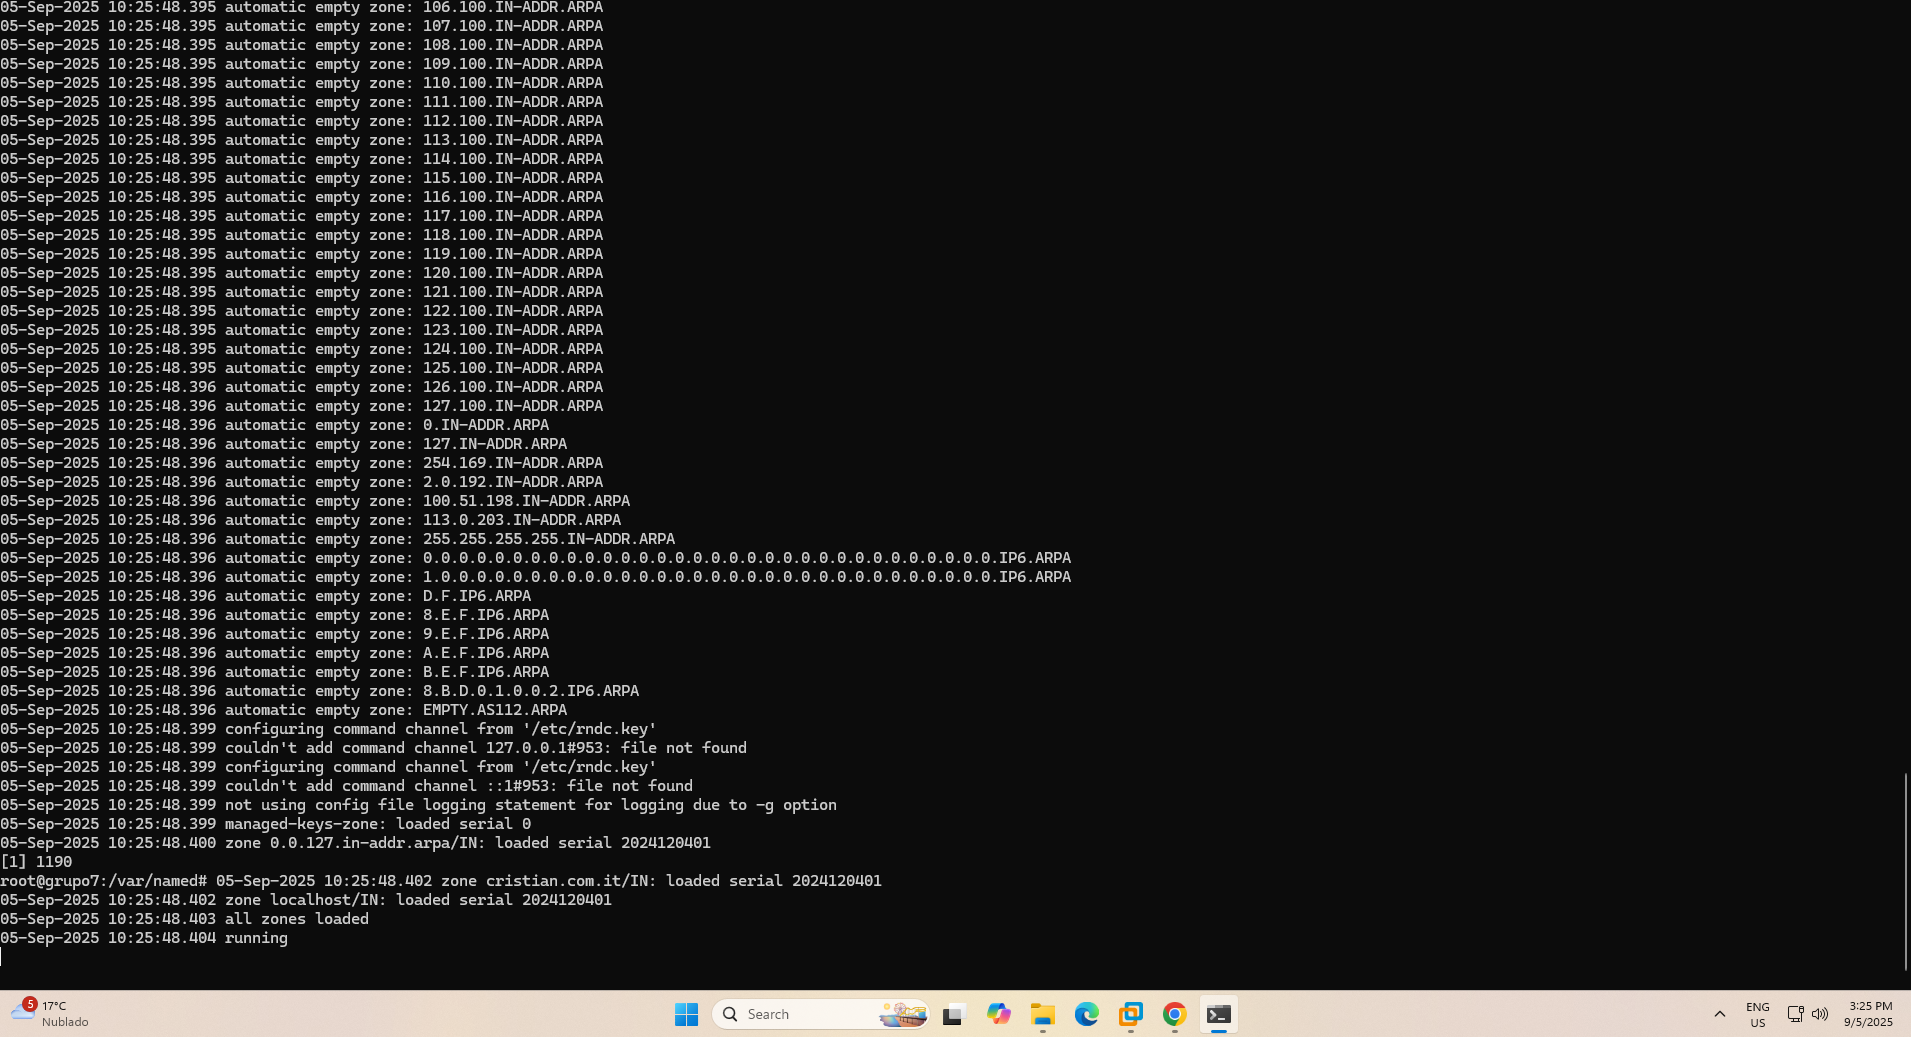
\includegraphics[keepaspectratio,alt={image.png}]{Third - DNS 263f56fc503e80ddb361c216e75fd3bf/image 24.png}}
\caption{image.png}
\end{figure}

\subsection{Step 10: Verify Service is
Running}\label{step-10-verify-service-is-running}

\begin{Shaded}
\begin{Highlighting}[]
\CommentTok{\# Check if process is running}
\ExtensionTok{solaris\#}\NormalTok{ ps }\AttributeTok{{-}ef} \KeywordTok{|} \FunctionTok{grep}\NormalTok{ named}

\CommentTok{\# Check if listening on port 53}
\ExtensionTok{solaris\#}\NormalTok{ netstat }\AttributeTok{{-}an} \KeywordTok{|} \FunctionTok{grep}\NormalTok{ :53}

\CommentTok{\# Expected output:}
\CommentTok{\# *.53                    *.*                    0      0 49152      0 LISTEN}
\end{Highlighting}
\end{Shaded}

\begin{figure}
\centering
\pandocbounded{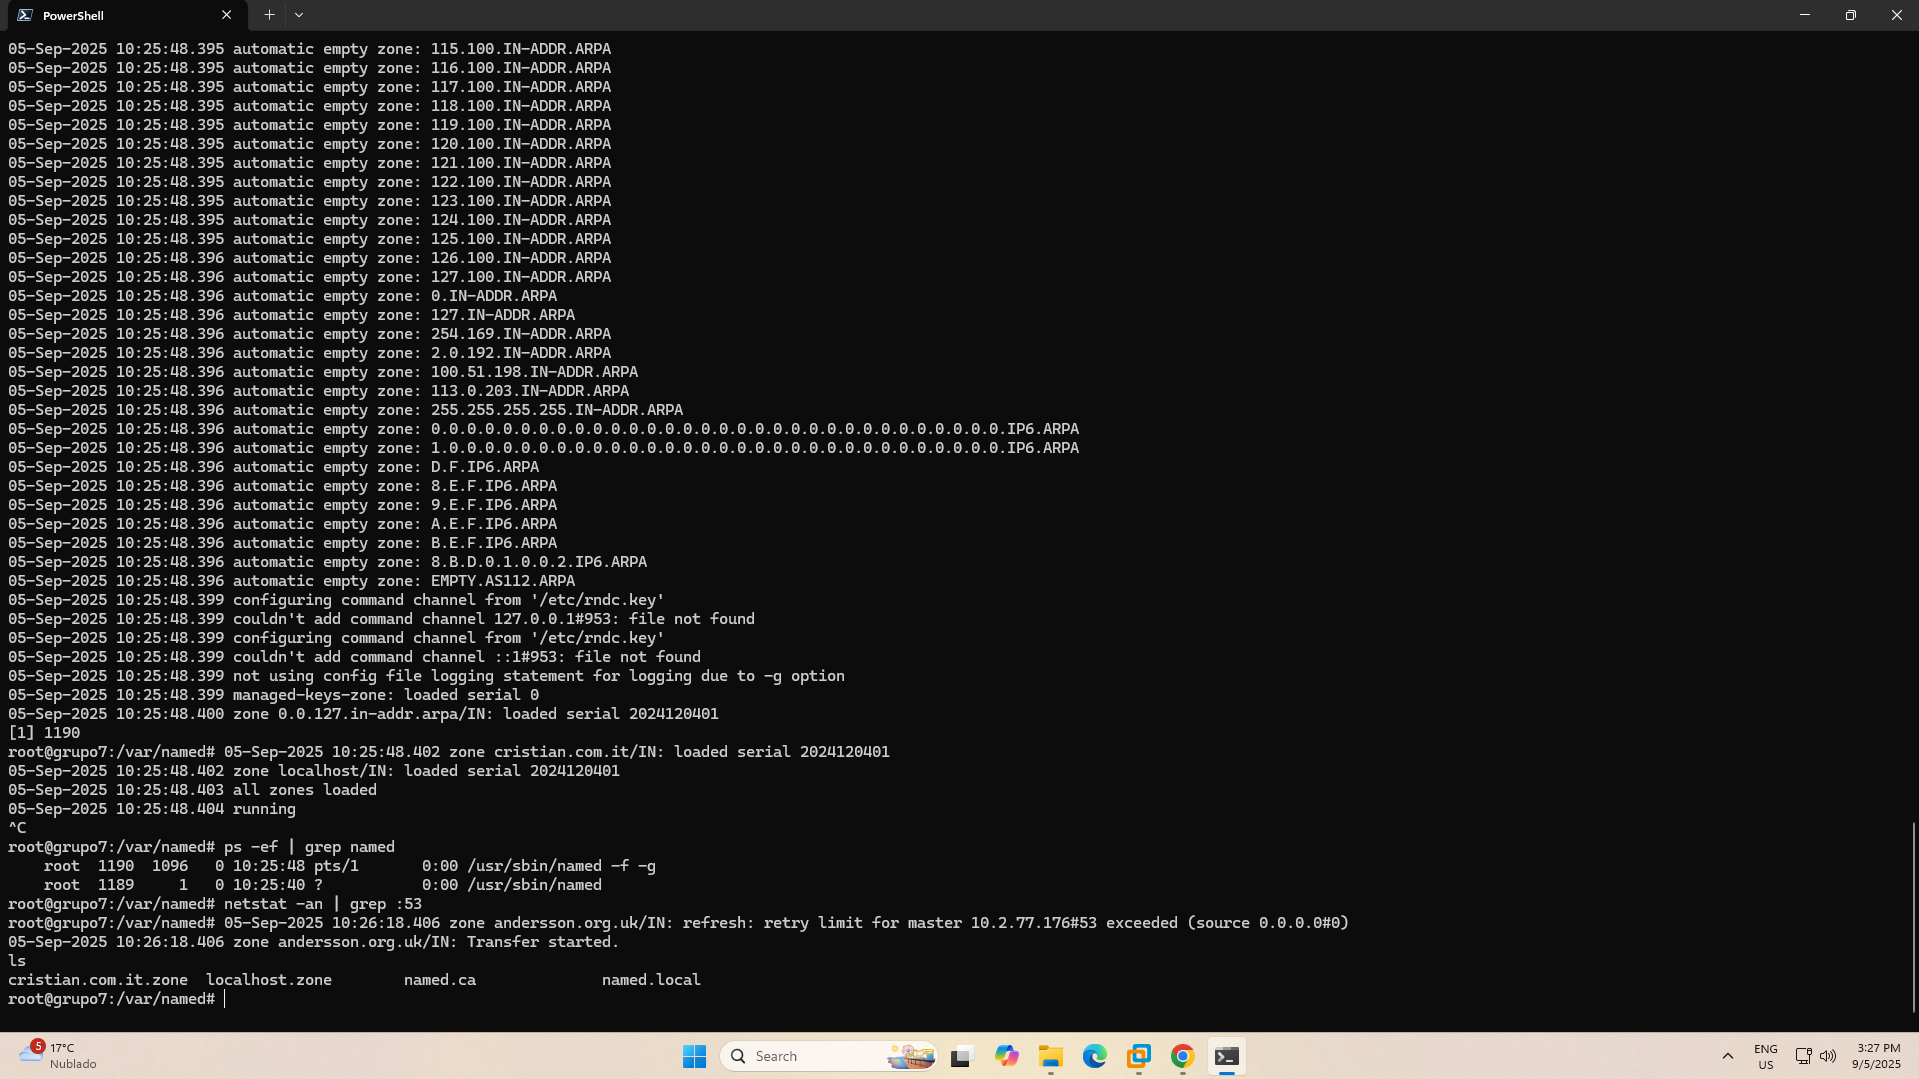
\includegraphics[keepaspectratio,alt={image.png}]{Third - DNS 263f56fc503e80ddb361c216e75fd3bf/image 25.png}}
\caption{image.png}
\end{figure}

\subsection{Step 11: Configure DNS
Resolution}\label{step-11-configure-dns-resolution}

\begin{Shaded}
\begin{Highlighting}[]
\ExtensionTok{solaris\#}\NormalTok{ nano /etc/resolv.conf}
\end{Highlighting}
\end{Shaded}

\textbf{Add these lines:}

\begin{Shaded}
\begin{Highlighting}[]
\ExtensionTok{nameserver}\NormalTok{ 127.0.0.1}
\ExtensionTok{nameserver}\NormalTok{ 10.2.77.178}
\ExtensionTok{nameserver}\NormalTok{ 10.2.77.176}
\end{Highlighting}
\end{Shaded}

\begin{figure}
\centering
\pandocbounded{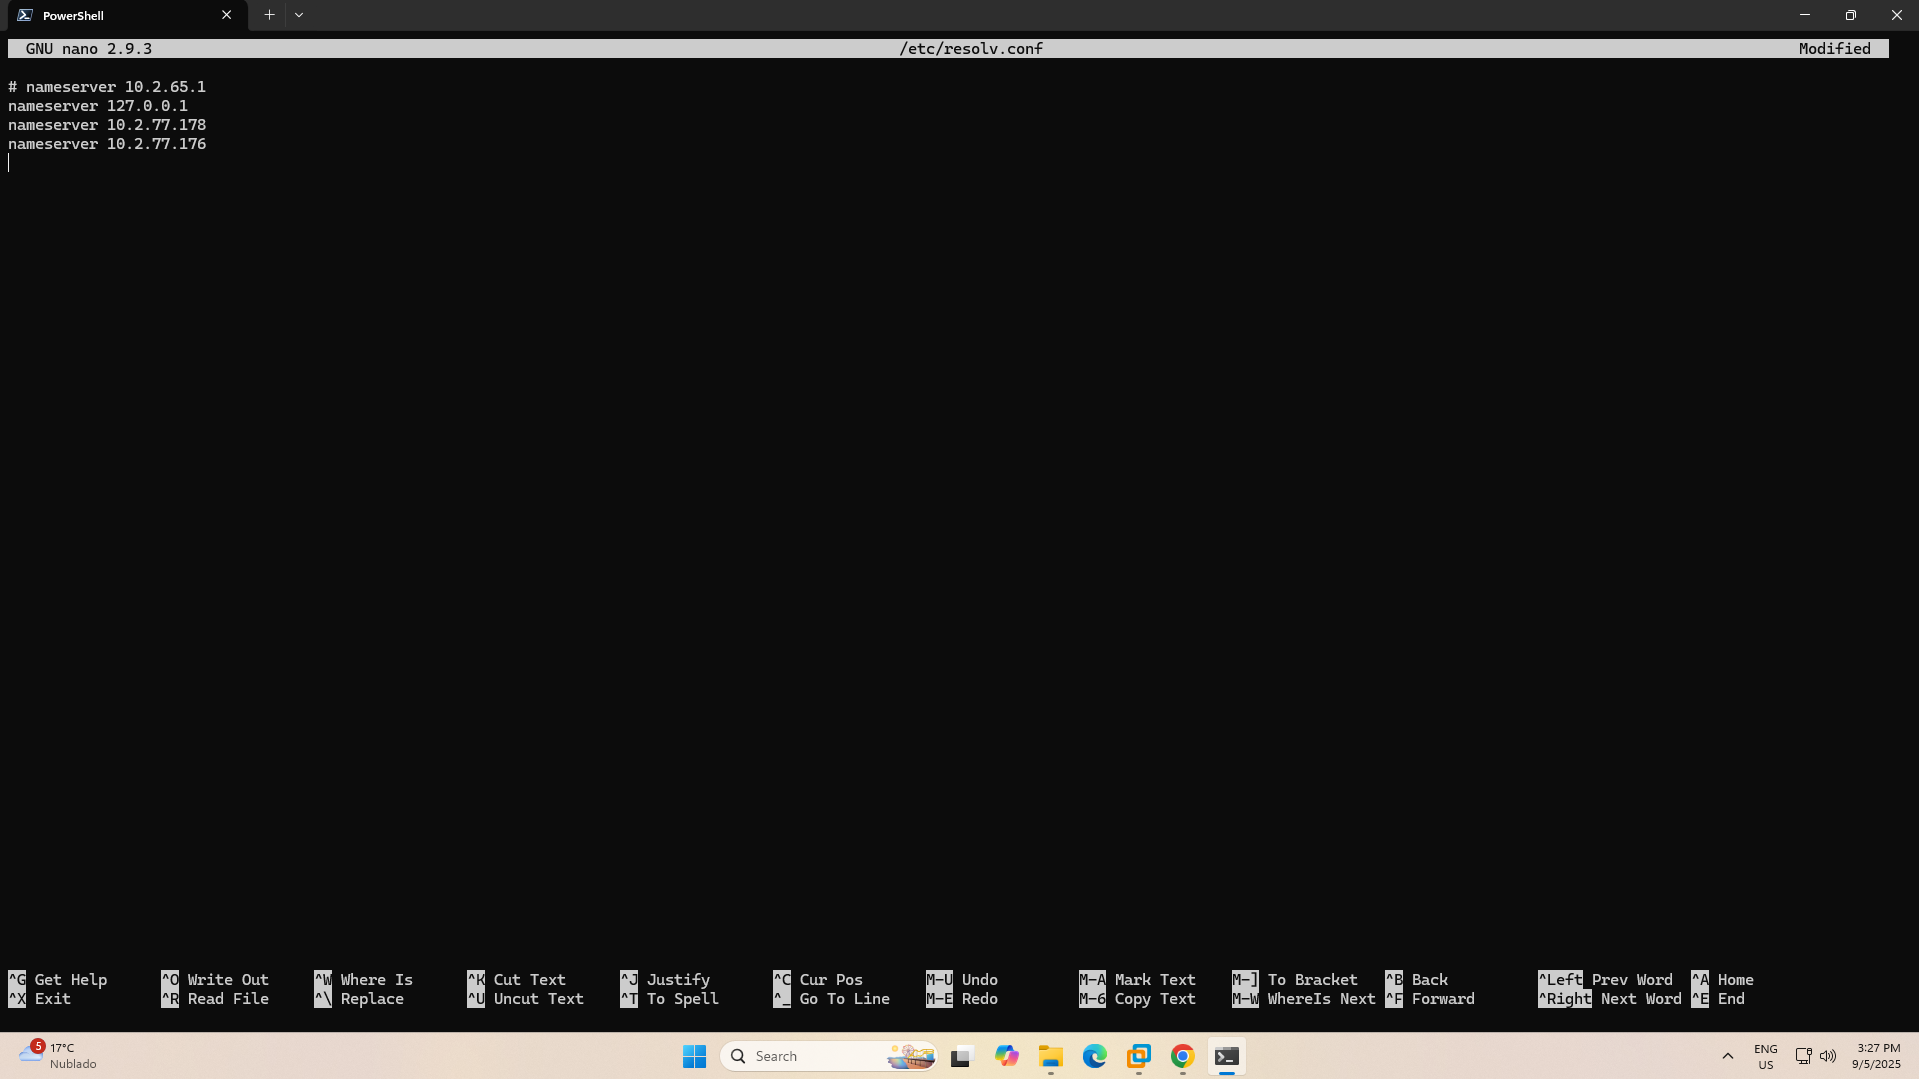
\includegraphics[keepaspectratio,alt={image.png}]{Third - DNS 263f56fc503e80ddb361c216e75fd3bf/image 26.png}}
\caption{image.png}
\end{figure}

\subsection{Step 12: Test Your DNS
Server}\label{step-12-test-your-dns-server}

\begin{Shaded}
\begin{Highlighting}[]
\CommentTok{\# Test local domain resolution}
\ExtensionTok{nslookup}\NormalTok{ dns.cristian.com.it}
\ExtensionTok{nslookup}\NormalTok{ www.cristian.com.it}
\ExtensionTok{nslookup}\NormalTok{ server1.cristian.com.it}

\CommentTok{\# Test secondary domain (should get from Slackware)}
\ExtensionTok{nslookup}\NormalTok{ server1.andersson.org.uk}

\CommentTok{\# Test internet resolution}
\ExtensionTok{nslookup}\NormalTok{ www.google.com}
\FunctionTok{ping}\NormalTok{ www.google.com}
\end{Highlighting}
\end{Shaded}

\begin{figure}
\centering
\pandocbounded{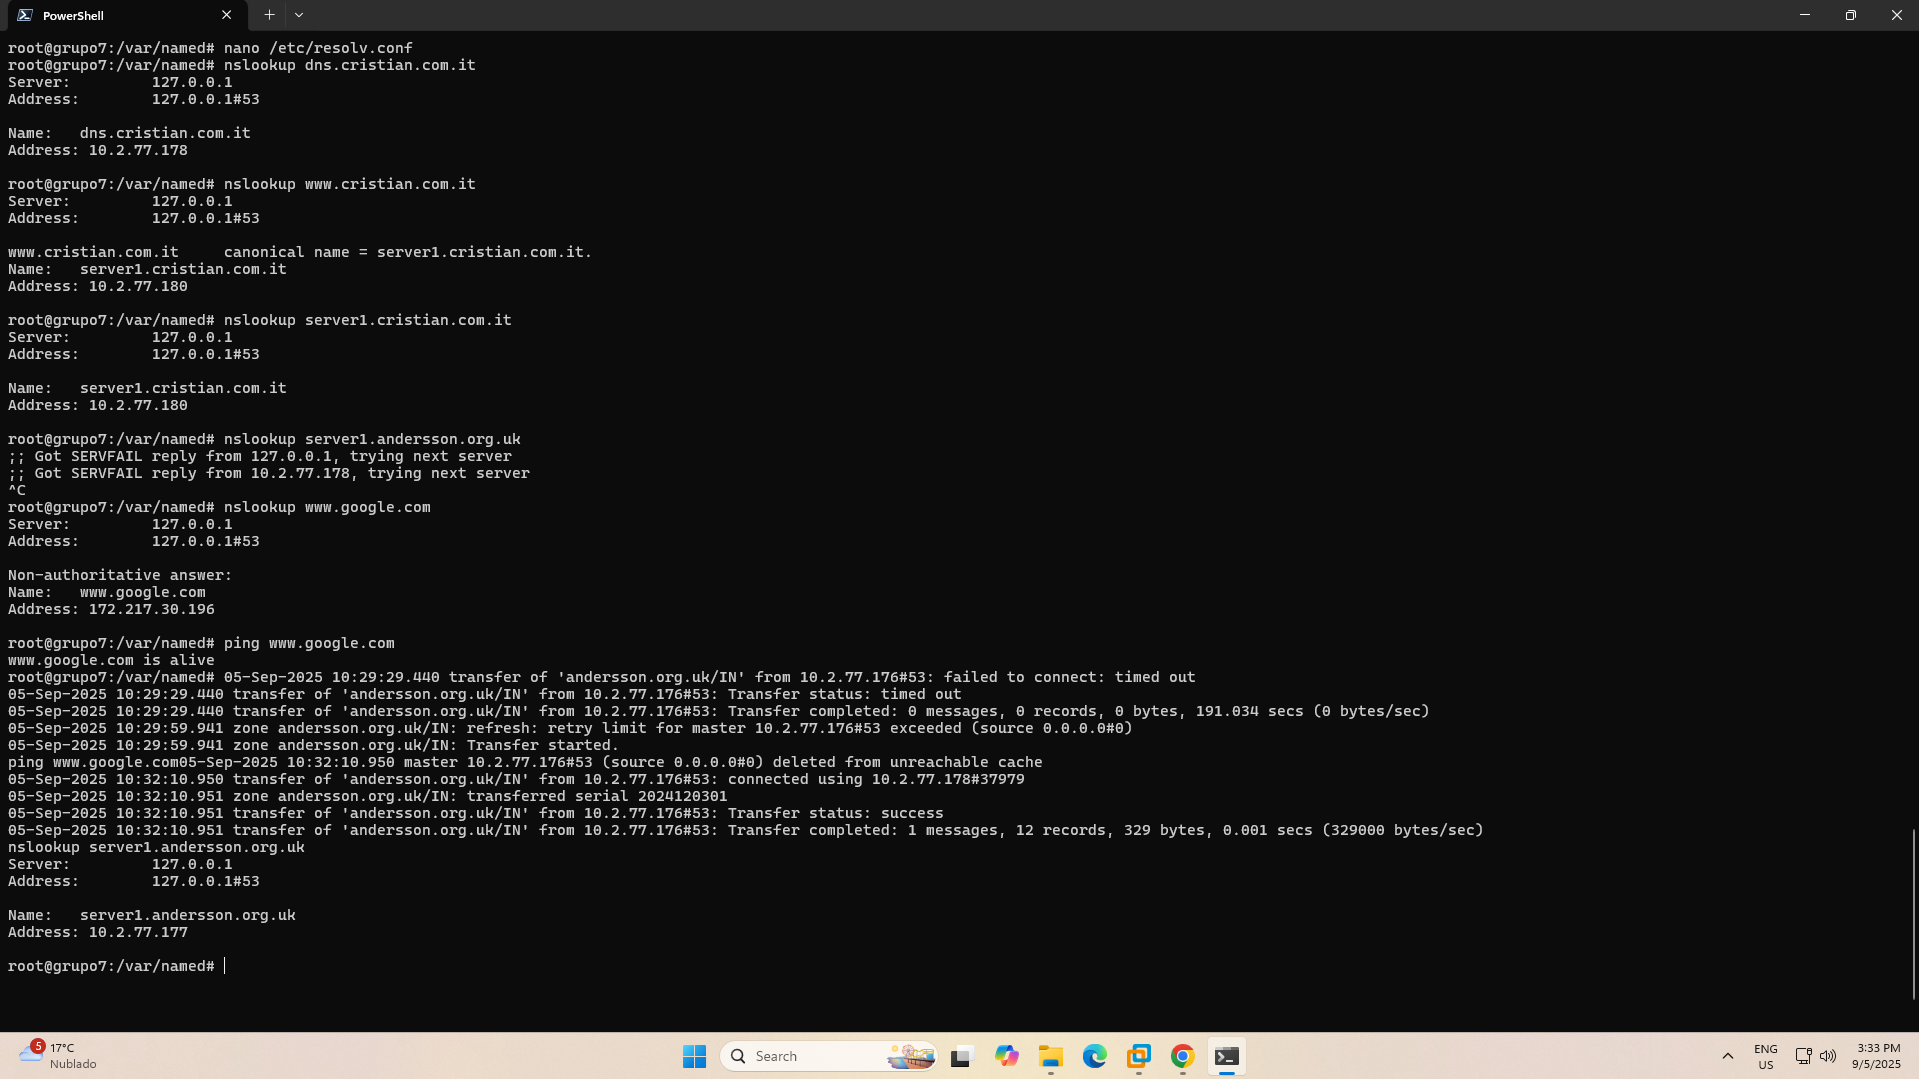
\includegraphics[keepaspectratio,alt={image.png}]{Third - DNS 263f56fc503e80ddb361c216e75fd3bf/image 27.png}}
\caption{image.png}
\end{figure}

\subsection{Step 13: Enable Automatic
Startup}\label{step-13-enable-automatic-startup}

\subsubsection{Method 1: Using SMF (Service Management Facility) -
Solaris
10+}\label{method-1-using-smf-service-management-facility---solaris-10}

\begin{Shaded}
\begin{Highlighting}[]
\CommentTok{\# Enable DNS service}
\ExtensionTok{solaris\#}\NormalTok{ svcadm enable svc:/network/dns/server:default}

\CommentTok{\# Check status}
\ExtensionTok{solaris\#}\NormalTok{ svcs }\AttributeTok{{-}l}\NormalTok{ dns/server}
\end{Highlighting}
\end{Shaded}

\begin{figure}
\centering
\pandocbounded{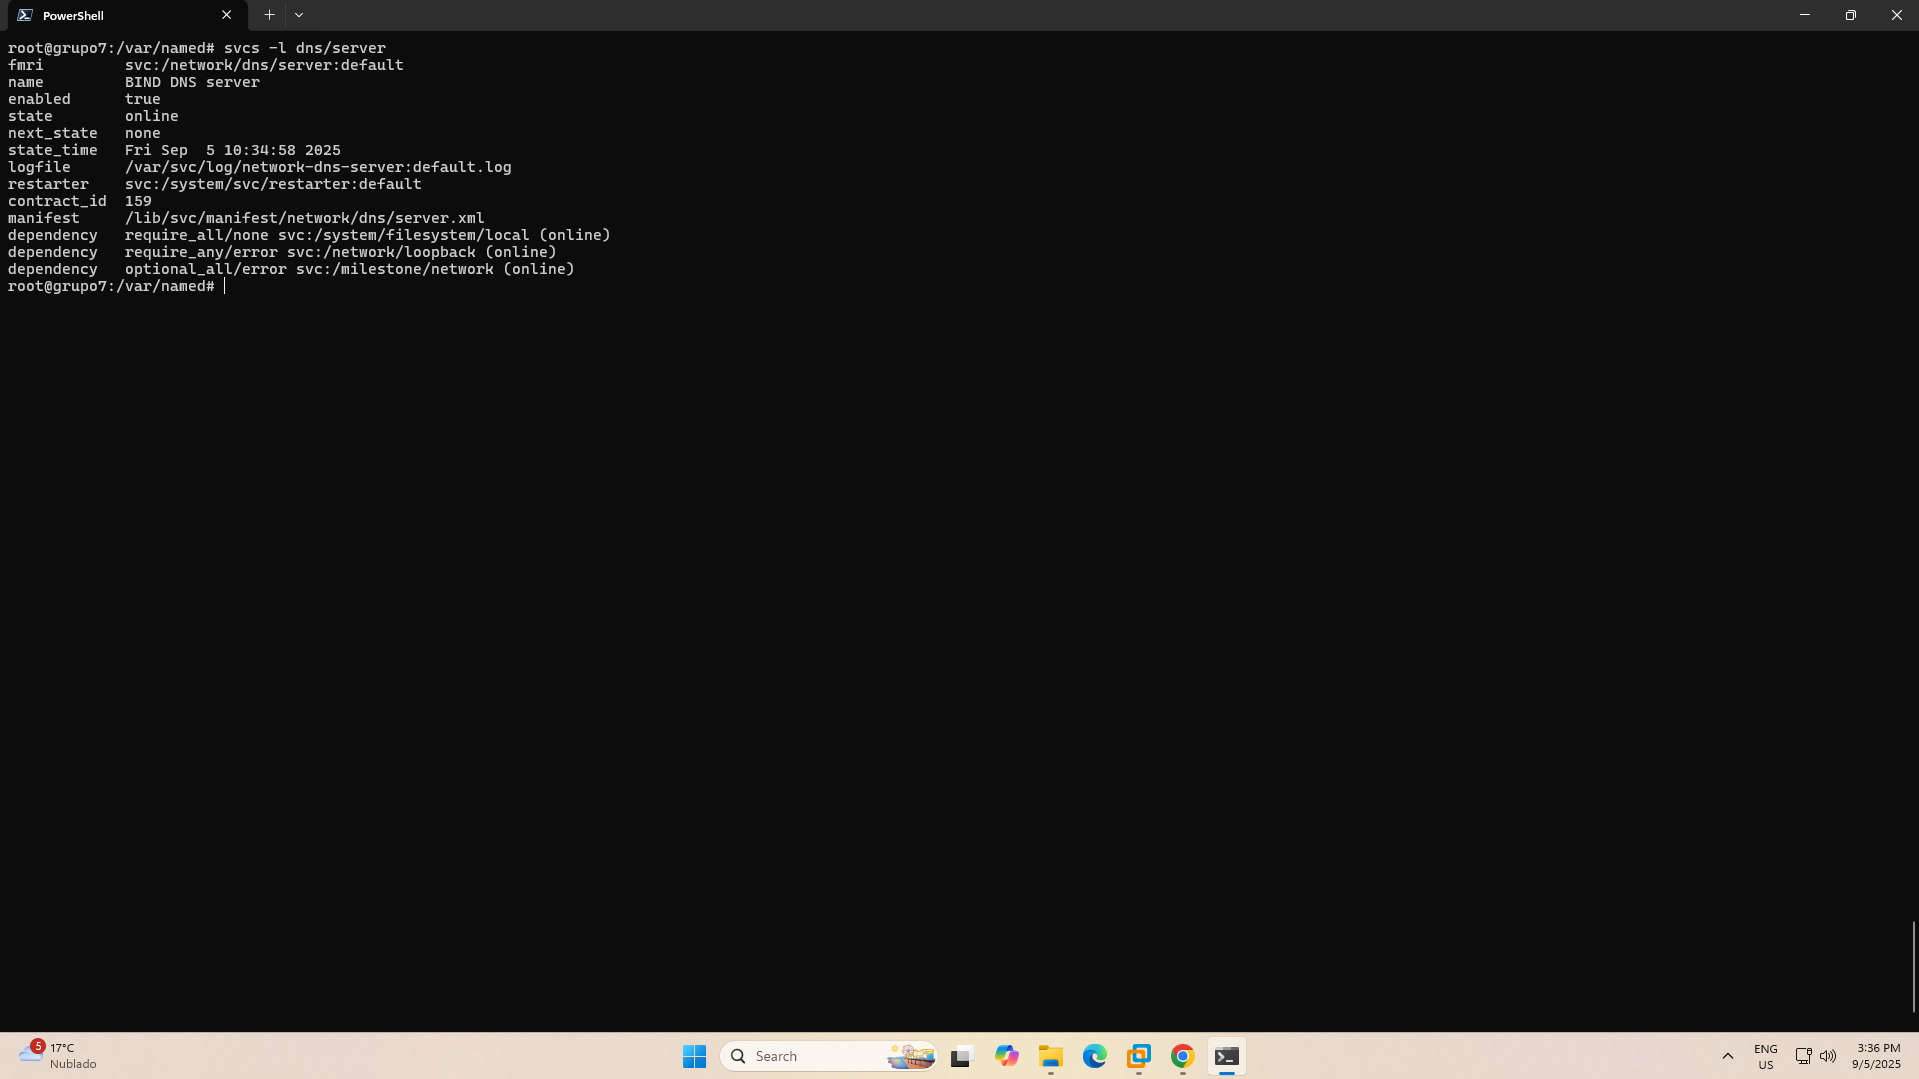
\includegraphics[keepaspectratio,alt={image.png}]{Third - DNS 263f56fc503e80ddb361c216e75fd3bf/image 28.png}}
\caption{image.png}
\end{figure}

\subsubsection{\texorpdfstring{\st{ethod 2: Traditional init
script}}{ethod 2: Traditional init script}}\label{ethod-2-traditional-init-script}

\begin{Shaded}
\begin{Highlighting}[]
\CommentTok{\# Create startup script}
\ExtensionTok{solaris\#}\NormalTok{ vi /etc/init.d/named}
\end{Highlighting}
\end{Shaded}

\textbf{\st{Content for /etc/init.d/named:}}

\begin{Shaded}
\begin{Highlighting}[]
\CommentTok{\#!/bin/sh}

\ControlFlowTok{case} \StringTok{"}\VariableTok{$1}\StringTok{"} \KeywordTok{in}
\SpecialStringTok{start}\KeywordTok{)}
    \BuiltInTok{echo} \StringTok{"Starting BIND DNS server..."}
    \ExtensionTok{/usr/sbin/named}
    \ControlFlowTok{;;}
\SpecialStringTok{stop}\KeywordTok{)}
    \BuiltInTok{echo} \StringTok{"Stopping BIND DNS server..."}
    \ExtensionTok{pkill}\NormalTok{ named}
    \ControlFlowTok{;;}
\SpecialStringTok{restart}\KeywordTok{)}
    \VariableTok{$0}\NormalTok{ stop}
    \FunctionTok{sleep}\NormalTok{ 2}
    \VariableTok{$0}\NormalTok{ start}
    \ControlFlowTok{;;}
\PreprocessorTok{*}\KeywordTok{)}
    \BuiltInTok{echo} \StringTok{"Usage: }\VariableTok{$0}\StringTok{ \{start|stop|restart\}"}
    \BuiltInTok{exit}\NormalTok{ 1}
    \ControlFlowTok{;;}
\ControlFlowTok{esac}
\end{Highlighting}
\end{Shaded}

\begin{Shaded}
\begin{Highlighting}[]
\CommentTok{\# Make executable and create links}
\ExtensionTok{solaris\#}\NormalTok{ chmod 755 /etc/init.d/named}
\ExtensionTok{solaris\#}\NormalTok{ ln }\AttributeTok{{-}s}\NormalTok{ /etc/init.d/named /etc/rc2.d/S85named}
\ExtensionTok{solaris\#}\NormalTok{ ln }\AttributeTok{{-}s}\NormalTok{ /etc/init.d/named /etc/rc1.d/K15named}
\end{Highlighting}
\end{Shaded}

\subsection{Step 14: Final
Verification}\label{step-14-final-verification}

After reboot, test everything:

\begin{Shaded}
\begin{Highlighting}[]
\CommentTok{\# Check service status}
\ExtensionTok{solaris\#}\NormalTok{ ps }\AttributeTok{{-}ef} \KeywordTok{|} \FunctionTok{grep}\NormalTok{ named}
\ExtensionTok{solaris\#}\NormalTok{ netstat }\AttributeTok{{-}an} \KeywordTok{|} \FunctionTok{grep}\NormalTok{ :53}

\CommentTok{\# Test all domains}
\ExtensionTok{solaris\#}\NormalTok{ nslookup dns.cristian.com.it}
\ExtensionTok{solaris\#}\NormalTok{ nslookup www.cristian.com.it}
\ExtensionTok{solaris\#}\NormalTok{ nslookup mail.cristian.com.it}
\ExtensionTok{solaris\#}\NormalTok{ nslookup server1.andersson.org.uk}
\ExtensionTok{solaris\#}\NormalTok{ ping www.google.com}
\end{Highlighting}
\end{Shaded}

\begin{figure}
\centering
\pandocbounded{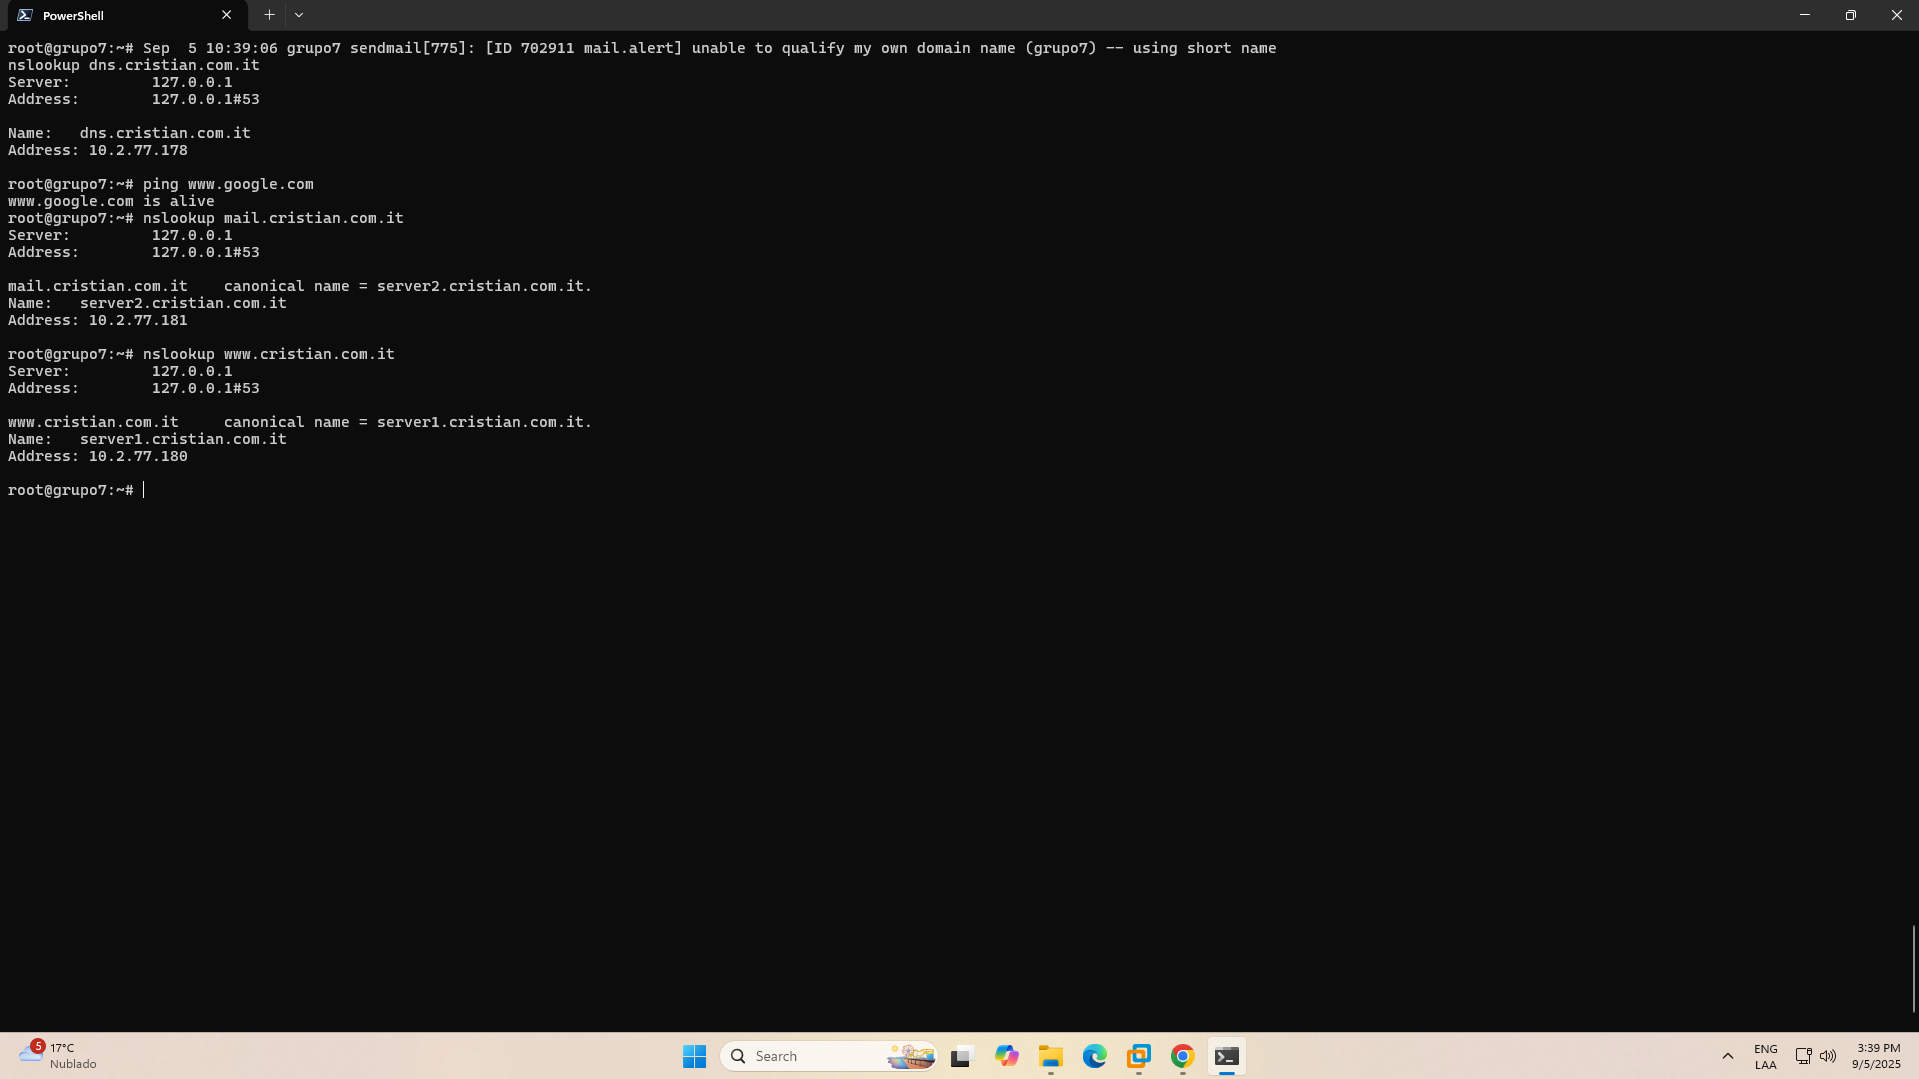
\includegraphics[keepaspectratio,alt={image.png}]{Third - DNS 263f56fc503e80ddb361c216e75fd3bf/image 29.png}}
\caption{image.png}
\end{figure}

\subsection{Summary}\label{summary}

Your Solaris server is now configured as:

\begin{itemize}
\tightlist
\item
  ✅ \textbf{Primary DNS} for \texttt{cristian.com.it}
\item
  ✅ \textbf{Secondary DNS} for \texttt{andersson.org.uk}
\item
  ✅ \textbf{Auto-start} on boot
\item
  ✅ \textbf{Zone transfers} enabled for replication
\end{itemize}

\textbf{Next Steps:} Configure Windows Server as secondary for both
domains!

\begin{center}\rule{0.5\linewidth}{0.5pt}\end{center}

\section{3. SLACKWARE AS SECONDARY DNS FOR SOLARIS
✅}\label{slackware-as-secondary-dns-for-solaris}

\subsubsection{\texorpdfstring{\textbf{Slackware
(10.2.77.176)}}{Slackware (10.2.77.176)}}\label{slackware-10.2.77.176}

\begin{itemize}
\tightlist
\item
  ✅ \textbf{Primary DNS} for \texttt{andersson.org.uk}
\item
  ✅ Auto-start configured
\end{itemize}

\subsubsection{\texorpdfstring{\textbf{Solaris
(10.2.77.178)}}{Solaris (10.2.77.178)}}\label{solaris-10.2.77.178}

\begin{itemize}
\tightlist
\item
  ✅ \textbf{Primary DNS} for \texttt{cristian.com.it}
\item
  ✅ \textbf{Secondary DNS} for \texttt{andersson.org.uk} (gets zone
  from Slackware)
\item
  ✅ SMF auto-start configured
\end{itemize}

\subsection{What We Need to Do Now ⚡}\label{what-we-need-to-do-now}

\textbf{Update Slackware} to also be \textbf{Secondary DNS} for
\texttt{cristian.com.it} (getting zone from Solaris)

So Slackware will be:

\begin{itemize}
\tightlist
\item
  \textbf{Primary} for \texttt{andersson.org.uk}
\item
  \textbf{Secondary} for \texttt{cristian.com.it}
\end{itemize}

\subsection{Update Slackware
Configuration}\label{update-slackware-configuration}

Let's add the secondary zone configuration to your existing Slackware
setup:

\subsubsection{Step 1: Edit Slackware's
named.conf}\label{step-1-edit-slackwares-named.conf}

\begin{Shaded}
\begin{Highlighting}[]
\CommentTok{\# On Slackware machine}
\ExtensionTok{root@darkstar:\textasciitilde{}\#}\NormalTok{ nano /etc/named.conf}
\end{Highlighting}
\end{Shaded}

\textbf{Add this secondary zone section to your existing config:}

\begin{Shaded}
\begin{Highlighting}[]
\ExtensionTok{options}\NormalTok{ \{}
        \ExtensionTok{directory} \StringTok{"/var/named"}\KeywordTok{;}
        \ExtensionTok{allow{-}query}\NormalTok{ \{ any}\KeywordTok{;} \ErrorTok{\}}\KeywordTok{;}
        \ExtensionTok{recursion}\NormalTok{ yes}\KeywordTok{;}
\ErrorTok{\}}\KeywordTok{;}

\ExtensionTok{//}\NormalTok{ Root zone}
\ExtensionTok{zone} \StringTok{"."}\NormalTok{ IN \{}
        \BuiltInTok{type}\NormalTok{ hint}\KeywordTok{;}
        \FunctionTok{file} \StringTok{"caching{-}example/named.root"}\KeywordTok{;}
\ErrorTok{\}}\KeywordTok{;}

\ExtensionTok{//}\NormalTok{ PRIMARY zone for andersson.org.uk}
\ExtensionTok{zone} \StringTok{"andersson.org.uk"}\NormalTok{ IN \{}
        \BuiltInTok{type}\NormalTok{ master}\KeywordTok{;}
        \FunctionTok{file} \StringTok{"andersson.org.uk.zone"}\KeywordTok{;}
        \ExtensionTok{allow{-}transfer}\NormalTok{ \{ 10.2.77.178}\KeywordTok{;} \ErrorTok{\}}\KeywordTok{;}  \ExtensionTok{//}\NormalTok{ Allow Solaris to transfer}
\ErrorTok{\}}\KeywordTok{;}

\ExtensionTok{//}\NormalTok{ NEW: SECONDARY zone for cristian.com.it }\ErrorTok{(}\ExtensionTok{from}\NormalTok{ Solaris}\KeywordTok{)}
\ExtensionTok{zone} \StringTok{"cristian.com.it"}\NormalTok{ IN \{}
        \BuiltInTok{type}\NormalTok{ slave}\KeywordTok{;}
        \FunctionTok{file} \StringTok{"cristian.com.it.slave"}\KeywordTok{;}
        \ExtensionTok{masters}\NormalTok{ \{ 10.2.77.178}\KeywordTok{;} \ErrorTok{\}}\KeywordTok{;}
\ErrorTok{\}}\KeywordTok{;}

\ExtensionTok{//}\NormalTok{ Localhost zones}
\ExtensionTok{zone} \StringTok{"localhost"}\NormalTok{ IN \{}
        \BuiltInTok{type}\NormalTok{ master}\KeywordTok{;}
        \FunctionTok{file} \StringTok{"caching{-}example/localhost.zone"}\KeywordTok{;}
        \ExtensionTok{allow{-}update}\NormalTok{ \{ none}\KeywordTok{;} \ErrorTok{\}}\KeywordTok{;}
\ErrorTok{\}}\KeywordTok{;}

\ExtensionTok{zone} \StringTok{"0.0.127.in{-}addr.arpa"}\NormalTok{ IN \{}
        \BuiltInTok{type}\NormalTok{ master}\KeywordTok{;}
        \FunctionTok{file} \StringTok{"caching{-}example/named.local"}\KeywordTok{;}
        \ExtensionTok{allow{-}update}\NormalTok{ \{ none}\KeywordTok{;} \ErrorTok{\}}\KeywordTok{;}
\ErrorTok{\}}\KeywordTok{;}
\end{Highlighting}
\end{Shaded}

\begin{figure}
\centering
\pandocbounded{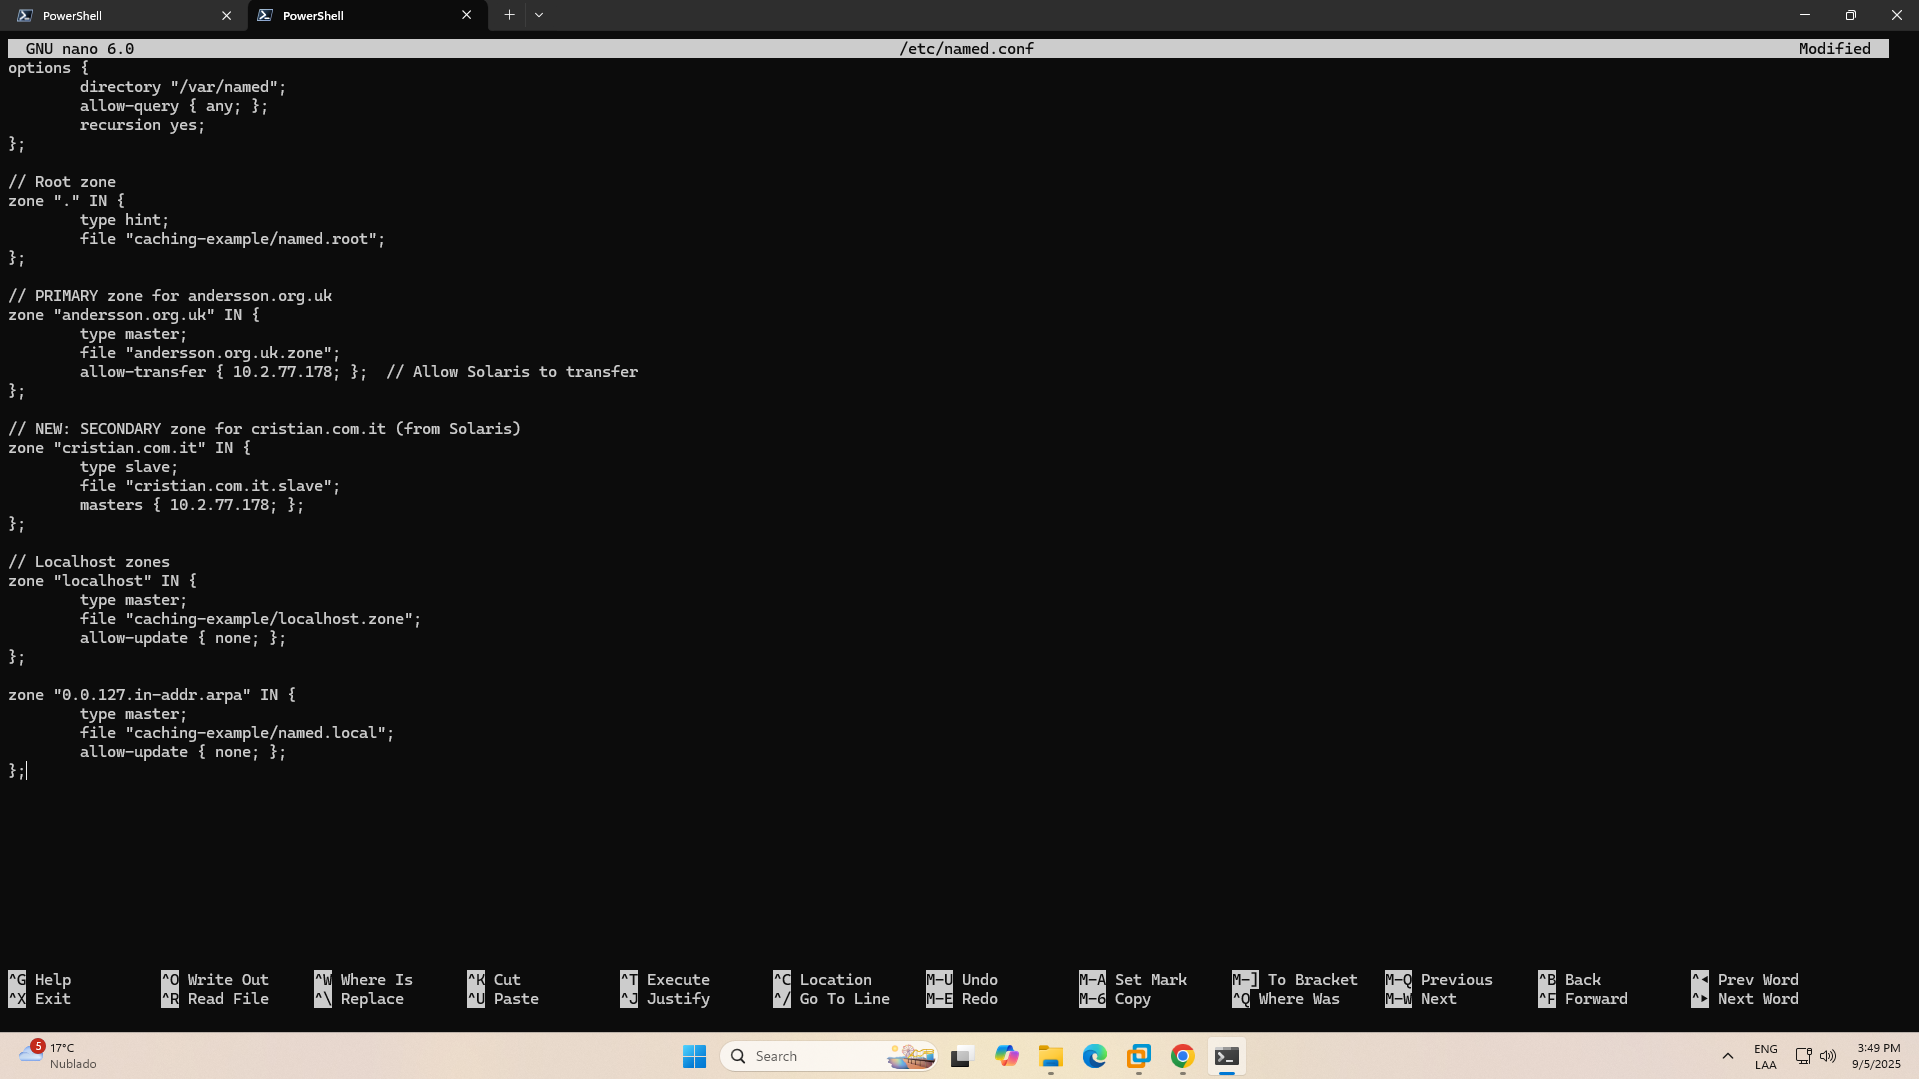
\includegraphics[keepaspectratio,alt={image.png}]{Third - DNS 263f56fc503e80ddb361c216e75fd3bf/image 30.png}}
\caption{image.png}
\end{figure}

\subsubsection{Step 2: Restart Slackware DNS
Service}\label{step-2-restart-slackware-dns-service}

\begin{Shaded}
\begin{Highlighting}[]
\ExtensionTok{root@darkstar:\textasciitilde{}\#}\NormalTok{ killall named}
\ExtensionTok{root@darkstar:\textasciitilde{}\#}\NormalTok{ /usr/sbin/named}
\end{Highlighting}
\end{Shaded}

\subsubsection{Step 3: Test Zone Transfer and
Resolution}\label{step-3-test-zone-transfer-and-resolution}

\begin{Shaded}
\begin{Highlighting}[]
\CommentTok{\# Test if it can resolve cristian.com.it domains (should get from Solaris)}
\ExtensionTok{root@darkstar:\textasciitilde{}\#}\NormalTok{ nslookup dns.cristian.com.it}
\ExtensionTok{root@darkstar:\textasciitilde{}\#}\NormalTok{ nslookup www.cristian.com.it}
\ExtensionTok{root@darkstar:\textasciitilde{}\#}\NormalTok{ nslookup server1.cristian.com.it}

\CommentTok{\# Test original andersson.org.uk still works}
    \ExtensionTok{root@darkstar:\textasciitilde{}\#}\NormalTok{ nslookup server1.andersson.org.uk}

\CommentTok{\# Check if the slave zone file was created}
\ExtensionTok{root@darkstar:\textasciitilde{}\#}\NormalTok{ ls }\AttributeTok{{-}la}\NormalTok{ /var/named/cristian.com.it.slave}
\end{Highlighting}
\end{Shaded}

\begin{figure}
\centering
\pandocbounded{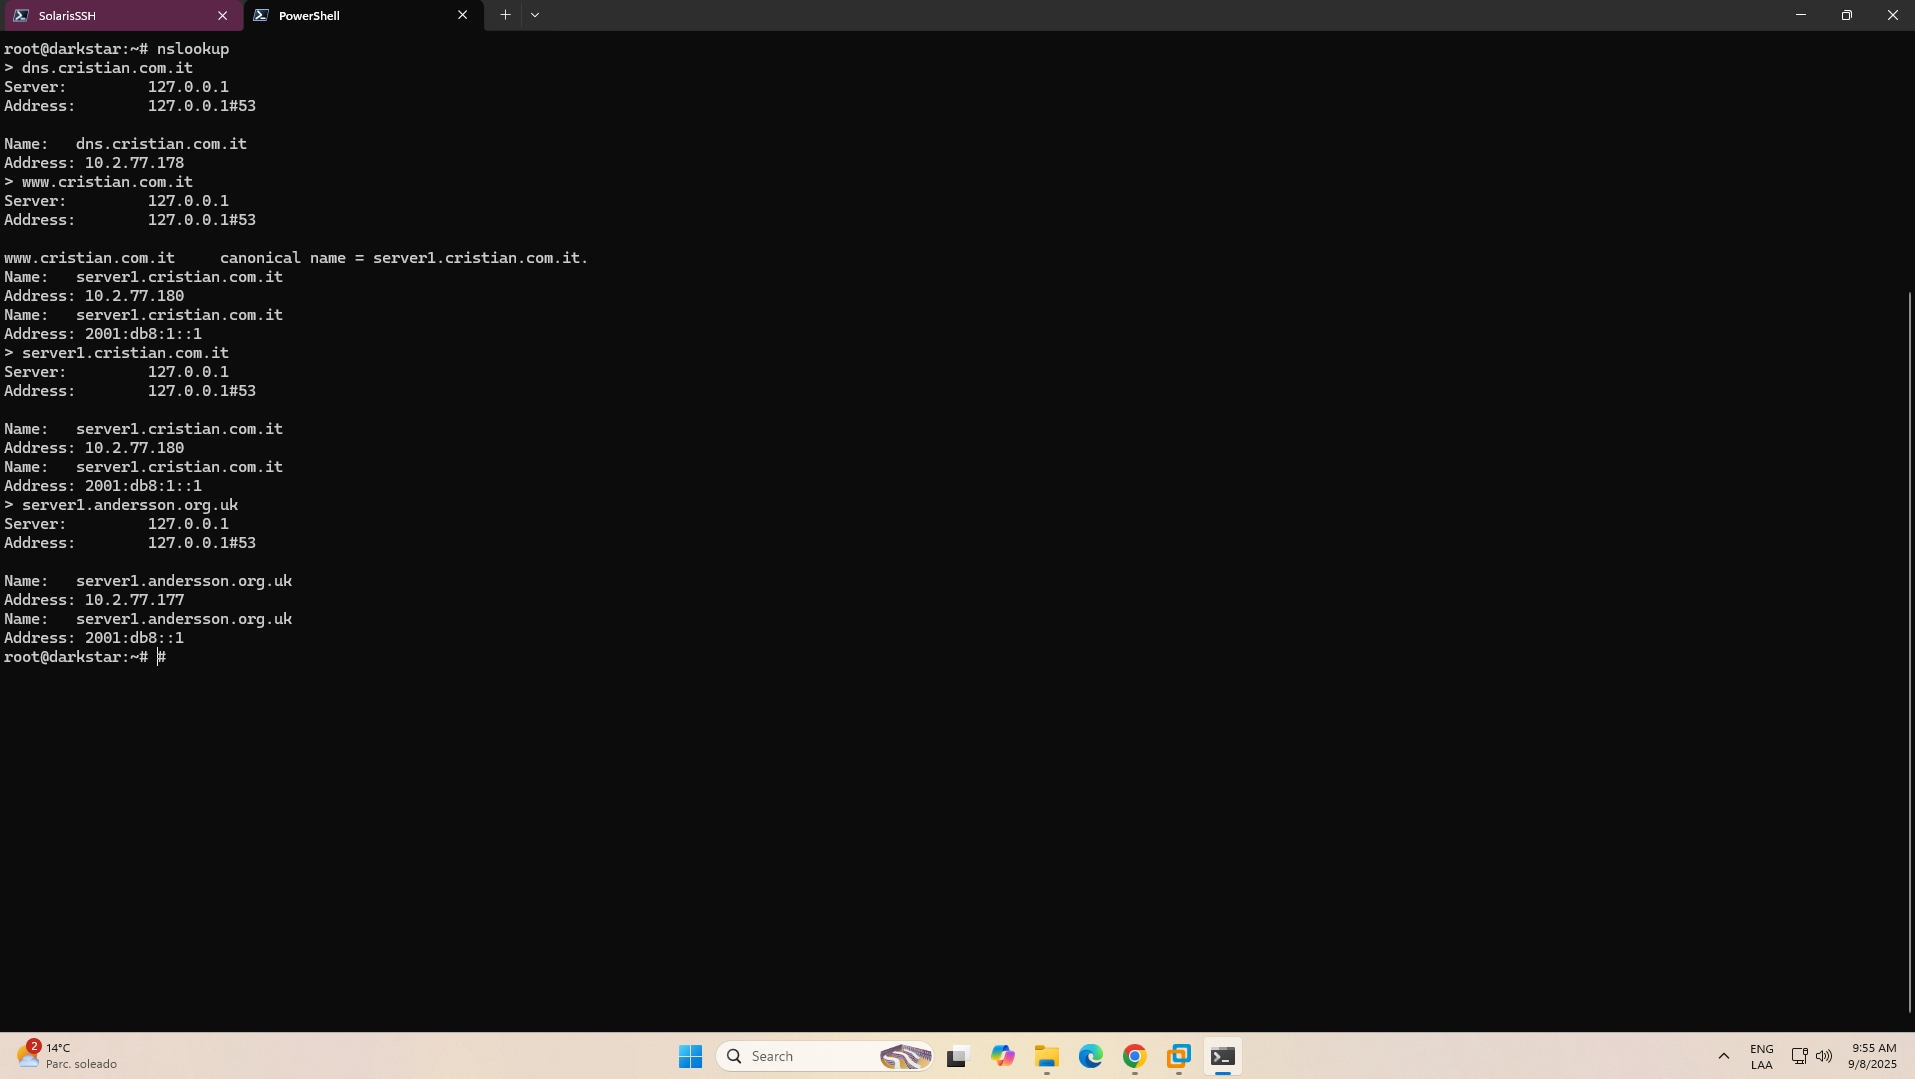
\includegraphics[keepaspectratio,alt={image.png}]{Third - DNS 263f56fc503e80ddb361c216e75fd3bf/image 31.png}}
\caption{image.png}
\end{figure}

\begin{figure}
\centering
\pandocbounded{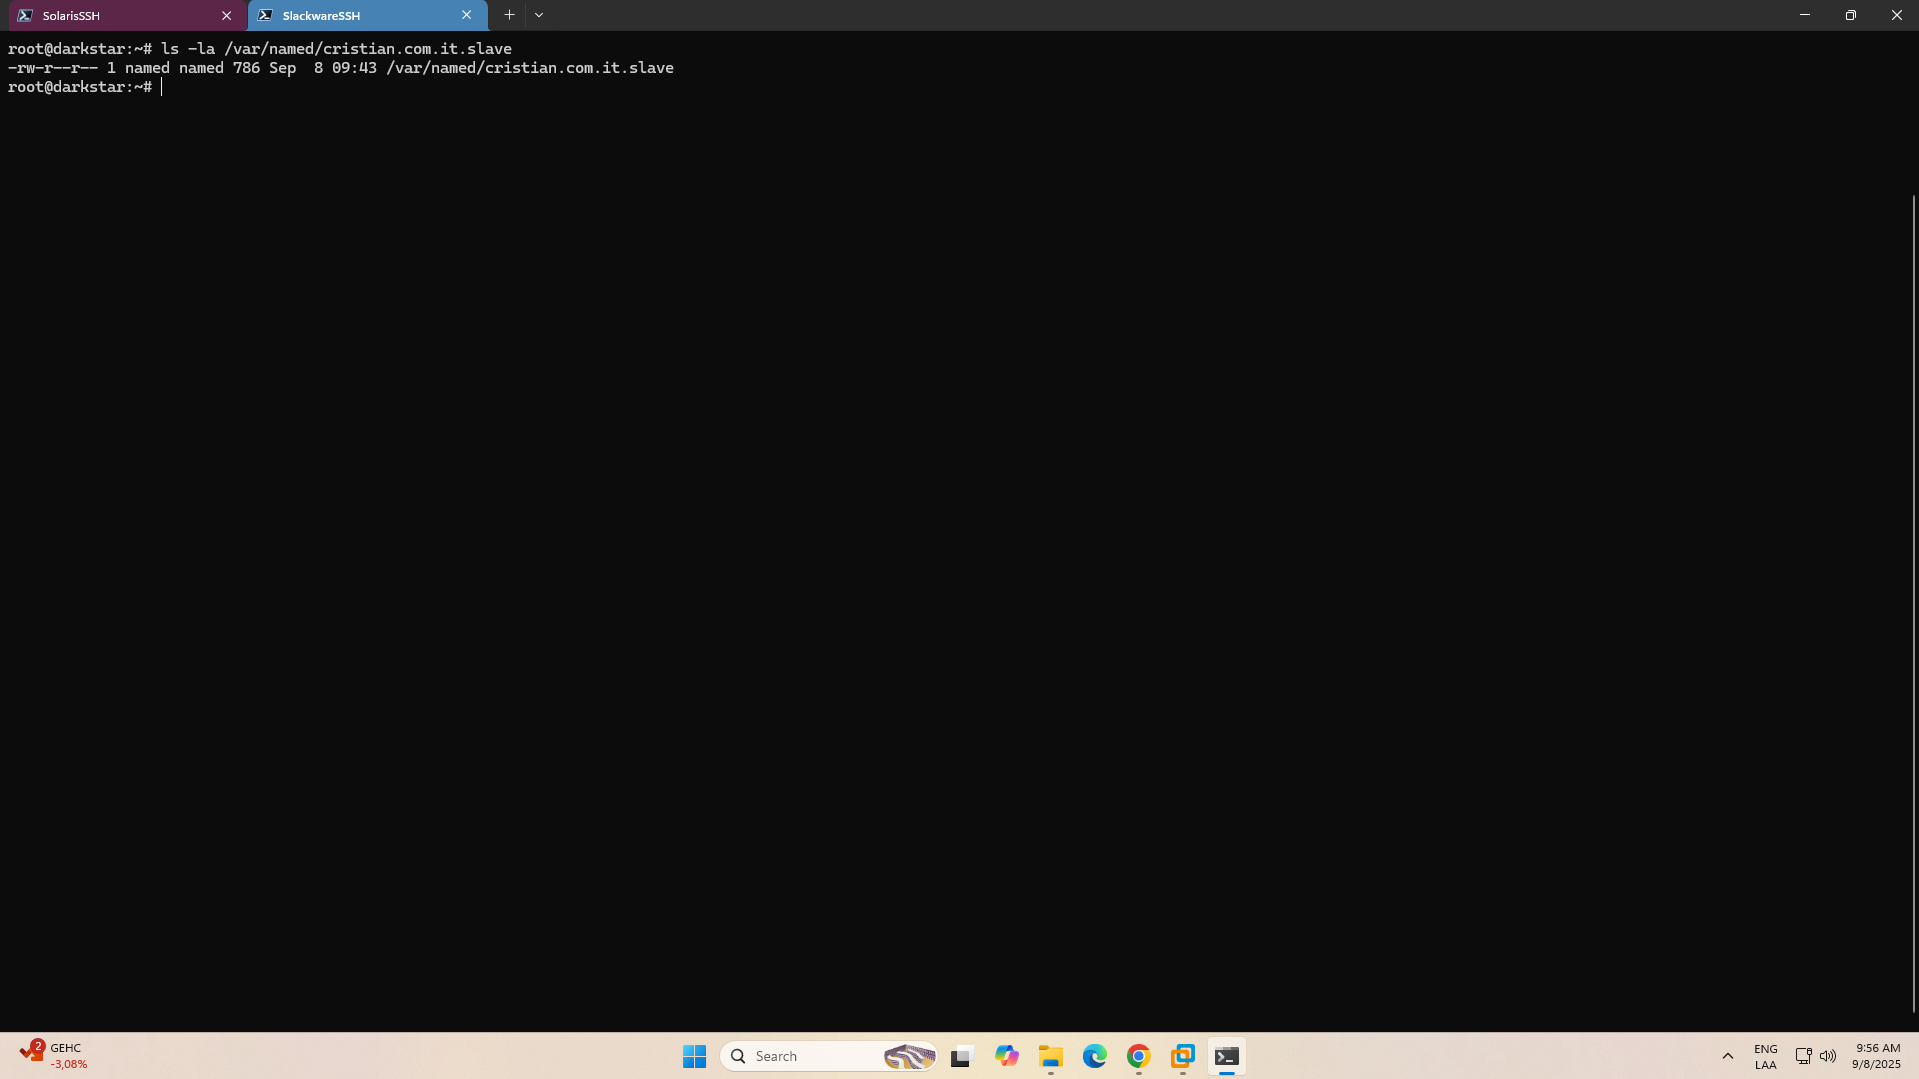
\includegraphics[keepaspectratio,alt={image.png}]{Third - DNS 263f56fc503e80ddb361c216e75fd3bf/image 32.png}}
\caption{image.png}
\end{figure}

\textbf{Try this configuration and tell me:}

\begin{enumerate}
\def\labelenumi{\arabic{enumi}.}
\tightlist
\item
  Does the named service restart without errors?
\item
  Can you resolve \texttt{cristian.com.it} domains from Slackware?
\item
  Was the \texttt{cristian.com.it.slave} file created?
\end{enumerate}

This will complete the bidirectional secondary DNS setup! 🎯

\href{Third\%20-\%20DNS\%20263f56fc503e80ddb361c216e75fd3bf/Lab\%20dns\%20explained\%20till\%20this\%20point\%20268f56fc503e808ea4b3f3d4d343e0a4.md}{Lab
dns explained till this point}

\href{Third\%20-\%20DNS\%20263f56fc503e80ddb361c216e75fd3bf/Lab\%20state\%20explained\%20268f56fc503e80ceb678fa071f071f39.md}{Lab
state explained}

\begin{center}\rule{0.5\linewidth}{0.5pt}\end{center}

\href{Third\%20-\%20DNS\%20263f56fc503e80ddb361c216e75fd3bf/Action\%20plan\%20268f56fc503e80e9aacffa65654c7332.md}{Action
plan}

\section{WINDOWS AS SLAVE FOR BOTH DNS SERVERS}\label{windows-as-slave-for-both-dns-servers}

\subsection{Windows Server 2025 - Secondary DNS Server Configuration}\label{windows-server-2025---secondary-dns-server-configuration}

\subsubsection{Overview}\label{overview-windows}

Configure Windows Server 2025 as \textbf{secondary DNS} for both domains:

\begin{itemize}
\tightlist
\item
  \textbf{Secondary for}: \texttt{andersson.org.uk} (Primary on Slackware 10.2.77.176)
\item
  \textbf{Secondary for}: \texttt{cristian.com.it} (Primary on Solaris 10.2.77.178)
\end{itemize}

\subsubsection{Prerequisites}\label{prerequisites-windows}

\begin{itemize}
\tightlist
\item
  Windows Server 2025 with GUI
\item
  Network connectivity to Slackware and Solaris servers
\item
  Administrative privileges
\end{itemize}

\begin{center}\rule{0.5\linewidth}{0.5pt}\end{center}

\subsection{Step 1: Install DNS Server Role}\label{step-1-install-dns-server-role}

\subsubsection{Method 1: Using Server Manager (GUI)}\label{method-1-using-server-manager-gui}

\begin{enumerate}
\def\labelenumi{\arabic{enumi}.}
\tightlist
\item
  \textbf{Open Server Manager}

  \begin{itemize}
  \tightlist
  \item
    Click \textbf{Start} → \textbf{Server Manager}
  \end{itemize}
\item
  \textbf{Add Roles and Features}

  \begin{itemize}
  \tightlist
  \item
    Click \textbf{"Add roles and features"}
  \item
    Click \textbf{Next} through the wizard
  \item
    Select \textbf{"Role-based or feature-based installation"}
  \item
    Click \textbf{Next}
  \end{itemize}
\item
  \textbf{Select Server Roles}

  \begin{itemize}
  \tightlist
  \item
    Check \textbf{"DNS Server"}
  \item
    When prompted, click \textbf{"Add Features"} to include management tools
  \item
    Click \textbf{Next} through remaining screens
  \item
    Click \textbf{"Install"}
  \end{itemize}
\end{enumerate}

\subsubsection{Method 2: Using PowerShell (Alternative)}\label{method-2-using-powershell-alternative}

\begin{lstlisting}[language=powershell]
# Open PowerShell as Administrator
Install-WindowsFeature DNS -IncludeManagementTools
\end{lstlisting}

\begin{center}\rule{0.5\linewidth}{0.5pt}\end{center}

\subsection{Step 2: Open DNS Manager}\label{step-2-open-dns-manager}

\begin{enumerate}
\def\labelenumi{\arabic{enumi}.}
\tightlist
\item
  \textbf{Open DNS Manager}

  \begin{itemize}
  \tightlist
  \item
    Start Menu → \textbf{Administrative Tools} → \textbf{DNS}
  \item
    Or: \textbf{Server Manager} → \textbf{Tools} → \textbf{DNS}
  \end{itemize}
\item
  \textbf{Connect to Local Server}

  \begin{itemize}
  \tightlist
  \item
    The local server should appear in the left panel
  \item
    If not, right-click \textbf{"DNS"} → \textbf{"Connect to DNS Server"} → \textbf{"This computer"}
  \end{itemize}
\end{enumerate}

\begin{center}\rule{0.5\linewidth}{0.5pt}\end{center}

\subsection{Step 3: Configure Secondary Zone for andersson.org.uk}\label{step-3-configure-secondary-zone-for-andersson.org.uk}

\subsubsection{3.1 Create Secondary Zone}\label{create-secondary-zone-andersson}

\begin{enumerate}
\def\labelenumi{\arabic{enumi}.}
\tightlist
\item
  \textbf{Right-click "Forward Lookup Zones"}

  \begin{itemize}
  \tightlist
  \item
    Select \textbf{"New Zone..."}
  \end{itemize}
\item
  \textbf{Zone Type Selection}

  \begin{itemize}
  \tightlist
  \item
    Select \textbf{"Secondary zone"}
  \item
    Click \textbf{Next}
  \end{itemize}
\item
  \textbf{Zone Name}

  \begin{itemize}
  \tightlist
  \item
    Enter: \texttt{andersson.org.uk}
  \item
    Click \textbf{Next}
  \end{itemize}
\item
  \textbf{Master DNS Servers}

  \begin{itemize}
  \tightlist
  \item
    Click \textbf{"Add..."}
  \item
    Enter IP: \texttt{10.2.77.176} (Slackware server)
  \item
    Click \textbf{OK}
  \item
    Click \textbf{Next}
  \end{itemize}
\item
  \textbf{Complete the Wizard}

  \begin{itemize}
  \tightlist
  \item
    Click \textbf{"Finish"}
  \end{itemize}
\end{enumerate}

\subsubsection{3.2 Verify Zone Transfer}\label{verify-zone-transfer-andersson}

\begin{enumerate}
\def\labelenumi{\arabic{enumi}.}
\tightlist
\item
  \textbf{Check Zone Status}

  \begin{itemize}
  \tightlist
  \item
    Expand \textbf{"Forward Lookup Zones"}
  \item
    Click on \textbf{"andersson.org.uk"}
  \item
    You should see records transferred from Slackware
  \end{itemize}
\item
  \textbf{Force Zone Transfer (if needed)}

  \begin{itemize}
  \tightlist
  \item
    Right-click \textbf{"andersson.org.uk"}
  \item
    Select \textbf{"Transfer from Master"}
  \end{itemize}
\end{enumerate}

\begin{center}\rule{0.5\linewidth}{0.5pt}\end{center}

\subsection{Step 4: Configure Secondary Zone for cristian.com.it}\label{step-4-configure-secondary-zone-for-cristian.com.it}

\subsubsection{4.1 Create Secondary Zone}\label{create-secondary-zone-cristian}

\begin{enumerate}
\def\labelenumi{\arabic{enumi}.}
\tightlist
\item
  \textbf{Right-click "Forward Lookup Zones"}

  \begin{itemize}
  \tightlist
  \item
    Select \textbf{"New Zone..."}
  \end{itemize}
\item
  \textbf{Zone Type Selection}

  \begin{itemize}
  \tightlist
  \item
    Select \textbf{"Secondary zone"}
  \item
    Click \textbf{Next}
  \end{itemize}
\item
  \textbf{Zone Name}

  \begin{itemize}
  \tightlist
  \item
    Enter: \texttt{cristian.com.it}
  \item
    Click \textbf{Next}
  \end{itemize}
\item
  \textbf{Master DNS Servers}

  \begin{itemize}
  \tightlist
  \item
    Click \textbf{"Add..."}
  \item
    Enter IP: \texttt{10.2.77.178} (Solaris server)
  \item
    Click \textbf{OK}
  \item
    Click \textbf{Next}
  \end{itemize}
\item
  \textbf{Complete the Wizard}

  \begin{itemize}
  \tightlist
  \item
    Click \textbf{"Finish"}
  \end{itemize}
\end{enumerate}

\subsubsection{4.2 Verify Zone Transfer}\label{verify-zone-transfer-cristian}

\begin{enumerate}
\def\labelenumi{\arabic{enumi}.}
\tightlist
\item
  \textbf{Check Zone Status}

  \begin{itemize}
  \tightlist
  \item
    Click on \textbf{"cristian.com.it"}
  \item
    You should see records transferred from Solaris
  \end{itemize}
\item
  \textbf{Force Zone Transfer (if needed)}

  \begin{itemize}
  \tightlist
  \item
    Right-click \textbf{"cristian.com.it"}
  \item
    Select \textbf{"Transfer from Master"}
  \end{itemize}
\end{enumerate}

\begin{center}\rule{0.5\linewidth}{0.5pt}\end{center}

\subsection{Step 5: Configure DNS Server Settings}\label{step-5-configure-dns-server-settings}

\subsubsection{5.1 Configure Forwarders (for internet resolution)}\label{configure-forwarders}

\begin{enumerate}
\def\labelenumi{\arabic{enumi}.}
\tightlist
\item
  \textbf{Right-click your server name} in DNS Manager

  \begin{itemize}
  \tightlist
  \item
    Select \textbf{"Properties"}
  \end{itemize}
\item
  \textbf{Go to "Forwarders" tab}

  \begin{itemize}
  \tightlist
  \item
    Check \textbf{"Enable forwarders"}
  \item
    Click \textbf{"Add..."}
  \item
    Add: \texttt{8.8.8.8} (Google DNS)
  \item
    Add: \texttt{1.1.1.1} (Cloudflare DNS)
  \item
    Click \textbf{OK}
  \end{itemize}
\end{enumerate}

\subsubsection{5.2 Configure Recursion}\label{configure-recursion}

\begin{enumerate}
\def\labelenumi{\arabic{enumi}.}
\tightlist
\item
  \textbf{Go to "Advanced" tab}

  \begin{itemize}
  \tightlist
  \item
    Ensure \textbf{"Enable recursion"} is checked
  \item
    Click \textbf{OK}
  \end{itemize}
\end{enumerate}

\begin{center}\rule{0.5\linewidth}{0.5pt}\end{center}

\subsection{Step 6: Configure Network Settings}\label{step-6-configure-network-settings}

\subsubsection{6.1 Set DNS Server IP}\label{set-dns-server-ip}

\begin{enumerate}
\def\labelenumi{\arabic{enumi}.}
\tightlist
\item
  \textbf{Open Network Settings}

  \begin{itemize}
  \tightlist
  \item
    Control Panel → Network and Internet → Network Connections
  \item
    Right-click your network adapter → \textbf{Properties}
  \end{itemize}
\item
  \textbf{Configure IPv4}

  \begin{itemize}
  \tightlist
  \item
    Select \textbf{"Internet Protocol Version 4 (TCP/IPv4)"}
  \item
    Click \textbf{"Properties"}
  \item
    Select \textbf{"Use the following DNS server addresses"}
  \item
    \textbf{Preferred DNS server}: \texttt{127.0.0.1} (itself)
  \item
    \textbf{Alternate DNS server}: \texttt{10.2.77.176} (Slackware)
  \item
    Click \textbf{OK}
  \end{itemize}
\end{enumerate}

\begin{center}\rule{0.5\linewidth}{0.5pt}\end{center}

\subsection{Step 7: Test DNS Resolution}\label{step-7-test-dns-resolution}

\subsubsection{7.1 Test Using Command Prompt}\label{test-using-command-prompt}

\begin{lstlisting}[language=bash]
# Open Command Prompt as Administrator

# Test andersson.org.uk domain (from Slackware)
nslookup server1.andersson.org.uk
nslookup www.andersson.org.uk
nslookup dns.andersson.org.uk

# Test cristian.com.it domain (from Solaris)
nslookup server1.cristian.com.it
nslookup www.cristian.com.it
nslookup dns.cristian.com.it

# Test internet resolution
nslookup www.google.com
ping www.google.com
\end{lstlisting}

\subsubsection{7.2 Test Using PowerShell}\label{test-using-powershell}

\begin{lstlisting}[language=powershell]
# Test DNS resolution with PowerShell
Resolve-DnsName server1.andersson.org.uk
Resolve-DnsName www.cristian.com.it
Resolve-DnsName www.google.com

# Test specific DNS server
Resolve-DnsName server1.andersson.org.uk -Server 127.0.0.1
\end{lstlisting}

\begin{center}\rule{0.5\linewidth}{0.5pt}\end{center}

\subsection{Step 8: Monitor Zone Transfers}\label{step-8-monitor-zone-transfers}

\subsubsection{8.1 Check Event Logs}\label{check-event-logs}

\begin{enumerate}
\def\labelenumi{\arabic{enumi}.}
\tightlist
\item
  \textbf{Open Event Viewer}

  \begin{itemize}
  \tightlist
  \item
    Start → Administrative Tools → Event Viewer
  \item
    Navigate to: \textbf{Applications and Services Logs} → \textbf{DNS Server}
  \end{itemize}
\item
  \textbf{Look for Zone Transfer Events}

  \begin{itemize}
  \tightlist
  \item
    Look for successful zone transfer messages
  \item
    Check for any errors
  \end{itemize}
\end{enumerate}

\subsubsection{8.2 Monitor DNS Manager}\label{monitor-dns-manager}

\begin{enumerate}
\def\labelenumi{\arabic{enumi}.}
\tightlist
\item
  \textbf{Refresh Zones Regularly}

  \begin{itemize}
  \tightlist
  \item
    Right-click zones → \textbf{Reload} or \textbf{Transfer from Master}
  \end{itemize}
\item
  \textbf{Check Zone Serial Numbers}

  \begin{itemize}
  \tightlist
  \item
    Compare with primary servers to ensure updates
  \end{itemize}
\end{enumerate}

\begin{center}\rule{0.5\linewidth}{0.5pt}\end{center}

\subsection{Step 9: Configure Automatic Startup}\label{step-9-configure-automatic-startup}

\subsubsection{9.1 Verify DNS Service}\label{verify-dns-service}

\begin{enumerate}
\def\labelenumi{\arabic{enumi}.}
\tightlist
\item
  \textbf{Open Services}

  \begin{itemize}
  \tightlist
  \item
    Start → Run → \texttt{services.msc}
  \item
    Find \textbf{"DNS Server"} service
  \item
    Ensure \textbf{Startup Type} is \textbf{"Automatic"}
  \item
    Ensure \textbf{Status} is \textbf{"Running"}
  \end{itemize}
\item
  \textbf{Configure Service Recovery}

  \begin{itemize}
  \tightlist
  \item
    Right-click \textbf{"DNS Server"} → \textbf{Properties}
  \item
    Go to \textbf{"Recovery"} tab
  \item
    Set failure actions to restart the service
  \end{itemize}
\end{enumerate}

\begin{center}\rule{0.5\linewidth}{0.5pt}\end{center}

\subsection{Step 10: Advanced Configuration (Optional)}\label{step-10-advanced-configuration-optional}

\subsubsection{10.1 Configure Zone Transfer Security}\label{configure-zone-transfer-security}

\begin{enumerate}
\def\labelenumi{\arabic{enumi}.}
\tightlist
\item
  \textbf{Right-click each secondary zone}

  \begin{itemize}
  \tightlist
  \item
    Select \textbf{"Properties"}
  \item
    Go to \textbf{"Zone Transfers"} tab
  \item
    Select \textbf{"Only to the following servers"}
  \item
    Add trusted server IPs
  \end{itemize}
\end{enumerate}

\subsubsection{10.2 Configure Notifications}\label{configure-notifications}

\begin{enumerate}
\def\labelenumi{\arabic{enumi}.}
\tightlist
\item
  \textbf{On primary servers} (Slackware/Solaris)

  \begin{itemize}
  \tightlist
  \item
    Configure notify lists to include Windows Server IP
  \item
    This ensures immediate updates when zones change
  \end{itemize}
\end{enumerate}

\begin{center}\rule{0.5\linewidth}{0.5pt}\end{center}

\subsection{Troubleshooting Common Issues}\label{troubleshooting-common-issues}

\subsubsection{Issue 1: Zone Transfer Fails}\label{issue-1-zone-transfer-fails}

\textbf{Symptoms}: Empty zones, no records transferred

\textbf{Solutions}:
\begin{itemize}
\tightlist
\item
  Check network connectivity: \texttt{ping 10.2.77.176} and \texttt{ping 10.2.77.178}
\item
  Verify firewall settings on primary servers
\item
  Ensure zone transfer is allowed in primary server configs
\item
  Check DNS service is running on primary servers
\end{itemize}

\subsubsection{Issue 2: DNS Resolution Not Working}\label{issue-2-dns-resolution-not-working}

\textbf{Symptoms}: NXDOMAIN errors, timeouts

\textbf{Solutions}:
\begin{itemize}
\tightlist
\item
  Verify DNS server IP configuration
\item
  Check forwarders configuration
\item
  Restart DNS Server service
\item
  Clear DNS cache: \texttt{ipconfig /flushdns}
\end{itemize}

\subsubsection{Issue 3: Slow DNS Responses}\label{issue-3-slow-dns-responses}

\textbf{Symptoms}: Long resolution times

\textbf{Solutions}:
\begin{itemize}
\tightlist
\item
  Add more forwarders
\item
  Check network latency to primary servers
\item
  Verify DNS cache settings
\end{itemize}

\begin{center}\rule{0.5\linewidth}{0.5pt}\end{center}

\subsection{Expected Final Results}\label{expected-final-results}

After completing all steps, your Windows Server should:

\textbf{Resolve andersson.org.uk domains}:
\begin{itemize}
\tightlist
\item
  \texttt{server1.andersson.org.uk} → \texttt{10.2.77.177}
\item
  \texttt{www.andersson.org.uk} → points to server1
\item
  \texttt{dns.andersson.org.uk} → \texttt{10.2.77.176}
\end{itemize}

\textbf{Resolve cristian.com.it domains}:
\begin{itemize}
\tightlist
\item
  \texttt{server1.cristian.com.it} → \texttt{10.2.77.180}
\item
  \texttt{www.cristian.com.it} → points to server1
\item
  \texttt{dns.cristian.com.it} → \texttt{10.2.77.178}
\end{itemize}

\textbf{Resolve internet domains}:
\begin{itemize}
\tightlist
\item
  \texttt{www.google.com} → external IP
\item
  \texttt{www.microsoft.com} → external IP
\end{itemize}

\textbf{Provide redundancy}:
\begin{itemize}
\tightlist
\item
  If Slackware fails, Windows can still resolve \texttt{andersson.org.uk}
\item
  If Solaris fails, Windows can still resolve \texttt{cristian.com.it}
\end{itemize}

\begin{center}\rule{0.5\linewidth}{0.5pt}\end{center}

\subsection{Final Lab Architecture}\label{final-lab-architecture}

\begin{lstlisting}
DNS Lab - Complete Architecture

andersson.org.uk:
├── Primary:   Slackware (10.2.77.176)
├── Secondary: Solaris   (10.2.77.178)
└── Secondary: Windows   (your-windows-ip)

cristian.com.it:
├── Primary:   Solaris   (10.2.77.178)
├── Secondary: Slackware (10.2.77.176)
└── Secondary: Windows   (your-windows-ip)
\end{lstlisting}

\textbf{Your DNS lab will have complete high availability with 3 servers for each domain!}
